% Laboratory practice
% 2019-08-08 v. 0.1.0
% Juan Camilo Henao Londono
% Universität Duisburg-Essen
% \documentclass[12pt,a4paper,oneside]{article}
% % Default format
% \documentclass[12pt,twoside]{article}
% % Book format
% \documentclass[12pt, a4paper, twoside]{book}
\documentclass[12pt, a4paper, oneside]{book}
% include files that load packages and define macros
%%%%%%%%%%%%%%%%%%%%%%%%%%%%%%%%%%%%%%%%%
% University Assignment Title Page 
% LaTeX Template
% Version 1.0 (27/12/12)
%
% This template has been downloaded from:
% http://www.LaTeXTemplates.com
%
% Original author:
% WikiBooks (http://en.wikibooks.org/wiki/LaTeX/Title_Creation)
%
% License:
% CC BY-NC-SA 3.0 (http://creativecommons.org/licenses/by-nc-sa/3.0/)
% 
% Instructions for using this template:
% This title page is capable of being compiled as is. This is not useful for 
% including it in another document. To do this, you have two options: 
%
% 1) Copy/paste everything between \begin{document} and \end{document} 
% starting at \begin{titlepage} and paste this into another LaTeX file where you 
% want your title page.
% OR
% 2) Remove everything outside the \begin{titlepage} and \end{titlepage} and 
% move this file to the same directory as the LaTeX file you wish to add it to. 
% Then add \input{./title_page_1.tex} to your LaTeX file where you want your
% title page.
%
%----------------------------------------------------------------------------------------
%	PACKAGES AND OTHER DOCUMENT CONFIGURATIONS
%----------------------------------------------------------------------------------------
\usepackage{ifxetex}
\usepackage{textpos}
% \usepackage{cite}
\usepackage[round]{natbib}
% \usepackage{doi}
\usepackage{kpfonts}
\usepackage[a4paper,hmargin=2.8cm,vmargin=2.0cm,includeheadfoot]{geometry}
\usepackage{ifxetex}
\usepackage{stackengine}
\usepackage{tabularx,longtable,multirow,subfigure,caption}%hangcaption
\usepackage{fncylab} %formatting of labels
\usepackage{fancyhdr}
% \usepackage[svgnames,x11names,table]{xcolor}
\usepackage[dvipsnames]{xcolor}
\usepackage[tight,ugly]{units}
\usepackage{url}
\usepackage{float}
\usepackage[english]{babel}
\usepackage{amsmath}
\usepackage{mathtools}

% Alternative activation, when working with laptop,use draft settings !
\usepackage{graphicx}
% \usepackage[draft]{graphicx}

\usepackage[colorinlistoftodos]{todonotes}
\usepackage{dsfont}
\usepackage{epstopdf} % automatically replace .eps with .pdf in graphics
%\usepackage{backref}
\usepackage{array}
\usepackage{latexsym}
\usepackage{etoolbox}
\usepackage{enumerate} % for numbering with [a)] format 
\usepackage{blindtext} % Dummy text
\usepackage{ngerman}
\usepackage{listings,lstautogobble}
\usepackage{xparse}
\usepackage[utf8]{inputenc}
\DeclareFixedFont{\ttb}{T1}{txtt}{bx}{n}{12} % for bold
\DeclareFixedFont{\ttm}{T1}{txtt}{m}{n}{12}  % for normal
\usepackage{listings}
\usepackage{color} %red, green, blue, yellow, cyan, magenta, black, white
%\usepackage{subcaption}
\definecolor{mygreen}{RGB}{28,172,0} % color values Red, Green, Blue
\definecolor{mylilas}{RGB}{170,55,241}
\definecolor{deepblue}{rgb}{0,0,0.5}
\definecolor{deepred}{rgb}{0.6,0,0}
\definecolor{deepgreen}{rgb}{0,0.5,0}
\definecolor{codegreen}{rgb}{0,0.6,0}
\definecolor{codegray}{rgb}{0.5,0.5,0.5}
\definecolor{codepurple}{rgb}{0.58,0,0.82}
\definecolor{backcolour}{rgb}{0.95,0.95,0.92}
\definecolor{darkred}{rgb}{0.6,0.0,0.0}
\definecolor{darkgreen}{rgb}{0,0.50,0}
\definecolor{lightblue}{rgb}{0.0,0.42,0.91}
\definecolor{orange}{rgb}{0.99,0.48,0.13}
\definecolor{grass}{rgb}{0.18,0.80,0.18}
\definecolor{pink}{rgb}{0.97,0.15,0.45}
\definecolor{firebrick}{rgb}{0.7,0.13,0.13}
%\usepackage[export]{adjustbox}
%\usepackage{wrapfig}
\usepackage{rotating}
% \usepackage{tikz}
% \usepackage[detect-all]{siunitx}
\usepackage{graphicx}
\usepackage{adjustbox}
\usepackage[T1]{fontenc}
\usepackage{tikz-qtree}                
\usepackage{tikz}
  \usetikzlibrary{shapes,arrows,fit,calc,positioning}
  \tikzset{box/.style={draw, diamond, thick, text centered, minimum height=0.5cm, minimum width=1cm}}
  \tikzset{line/.style={draw, thick, -latex'}}
  \tikzset{every picture/.style={line width=0.75pt}} %set default line width to 0.75pt        
\usepackage{pgfplots}
  \pgfplotsset{compat=1.11,}
% \usepackage[linguistics]{forest}
% \usepackage[titles]{tocloft}
% \usepackage{pythonhighlight}
% \usepackage{minted}
% \usepackage{pygmentex}
\usepackage{notoccite}
% \usepackage[onehalfspacing]{setspace}
% \linespread{1.213}
\usepackage{setspace}
\usepackage{booktabs}
\newcommand{\tabitem}{~~\llap{\textbullet}~~}
\numberwithin{equation}{section}
\usepackage[inline]{enumitem}
\usepackage{titlesec}
\setcounter{tocdepth}{4} 
\setcounter{secnumdepth}{4}
\titleformat{\paragraph}
{\normalfont\normalsize\bfseries}{\theparagraph}{1em}{}
\titlespacing*{\paragraph}
{0pt}{3.25ex plus 1ex minus .2ex}{1.5ex plus .2ex}
% \usepackage{footnotebackref}
% Quick macros to type repeated texts
\setlength{\abovecaptionskip}{0pt} 

\newcommand{\scikit}{}
\def\scikit/{{\tt Scikit-Learn}}

\newcommand\bcitet[1]{\textbf{\citet{#1}}}
\newcommand\bcitep[1]{\textbf{\citep{#1}}}





% for code
% \lstset{frameround=fttt,language=SQL,numbers=left,breaklines=true}
\newcommand{\alen}{.7cm}
\newcommand{\blen}{1.5cm}
\newcommand{\clen}{2.4cm}


% \lstset{
%    frameround=fttt,
%    language=SQL,
%    numbers=left,
%    breaklines=true,
%    keywordstyle=\color{blue}\bfseries, 
%    basicstyle=\ttfamily\color{red},
%    numberstyle=\color{black}
%    }
% \lstMakeShortInline[columns=fixed]|

% \lstset{language=Matlab,%
%     basicstyle=\color{red},
%     breaklines=true,%
%     morekeywords={matlab2tikz},
%     keywordstyle=\color{blue},%
%     morekeywords=[2]{1}, keywordstyle=[2]{\color{black}},
%     identifierstyle=\color{black},%
%     stringstyle=\color{mylilas},
%     commentstyle=\color{mygreen},%
%     showstringspaces=false,%without this there will be a symbol in the places where there is a space
%     numbers=left,%
%     numberstyle={\tiny \color{black}},% size of the numbers
%     numbersep=9pt, % this defines how far the numbers are from the text
%     emph=[1]{for,end,break},emphstyle=[1]\color{red}, %some words to emphasise
%     emph=[2]{word1,word2}, emphstyle=[2]{style},    
% }

% Python style for highlighting
\newcommand\pythonstyle{\lstset{
language=Python,
% morekeywords={self},              % Add keywords here
morekeywords=[1]{,as,assert,nonlocal,with,yield,self,True,False,None,} % Python builtin
morekeywords=[2]{,__init__,__add__,__mul__,__div__,__sub__,__call__,__getitem__,__setitem__,__eq__,__ne__,__nonzero__,__rmul__,__radd__,__repr__,__str__,__get__,__truediv__,__pow__,__name__,__future__,__all__,}, % magic methods
morekeywords=[3]{,object,type,isinstance,copy,deepcopy,zip,enumerate,reversed,list,set,len,dict,tuple,range,xrange,append,execfile,real,imag,reduce,str,repr,}, % common functions
morekeywords=[4]{,Exception,NameError,IndexError,SyntaxError,TypeError,ValueError,OverflowError,ZeroDivisionError,}, % errors
morekeywords=[5]{,ode,fsolve,sqrt,exp,sin,cos,arctan,arctan2,arccos,pi, array,norm,solve,dot,arange,isscalar,max,sum,flatten,shape,reshape,find,any,all,abs,plot,linspace,legend,quad,polyval,polyfit,hstack,concatenate,vstack,column_stack,empty,zeros,ones,rand,vander,grid,pcolor,eig,eigs,eigvals,svd,qr,tan,det,logspace,roll,min,mean,cumsum,cumprod,diff,vectorize,lstsq,cla,eye,xlabel,ylabel,squeeze,}, % numpy / math
keywordstyle=[1]\color{blue},
keywordstyle=[2]\color{blue},
keywordstyle=[3]\color{grass},
keywordstyle=[4]\color{red},
keywordstyle=[5]\color{orange},
% keywordstyle=\color{blue},
emph={MyClass,__init__},          
emphstyle=\color{deepred},                            
backgroundcolor=\color{backcolour},   
commentstyle=\color{codegreen},
numberstyle=\tiny\color{codegray},
stringstyle=\color{codepurple},
basicstyle=\ttfamily\scriptsize,
breakatwhitespace=false,         
breaklines=true,                 
captionpos=b,                    
keepspaces=true,                 
numbers=left,                    
numbersep=5pt,                  
showspaces=false,                
showstringspaces=false,
showtabs=false,                  
tabsize=2,
autogobble = true
}}

% Python environment
\lstnewenvironment{python}[1][]
{
\pythonstyle
\lstset{#1}
}
{}

% Python for external files
\newcommand\pythonexternal[2][]{{
\pythonstyle
\lstinputlisting[#1]{#2}}}

% Python for inline
\newcommand\pythoninline[1]{{\pythonstyle\lstinline!#1!}}

% \lstdefinestyle{mystyle}{
%     backgroundcolor=\color{backcolour},   
%     commentstyle=\color{codegreen},
%     keywordstyle=\color{magenta},
%     numberstyle=\tiny\color{codegray},
%     stringstyle=\color{codepurple},
%     basicstyle=\ttfamily\scriptsize,
%     breakatwhitespace=false,         
%     breaklines=true,                 
%     captionpos=b,                    
%     keepspaces=true,                 
%     numbers=left,                    
%     numbersep=5pt,                  
%     showspaces=false,                
%     showstringspaces=false,
%     showtabs=false,                  
%     tabsize=2,
%     autogobble = true
% }


\ifxetex
\usepackage{fontspec}
\setmainfont[Scale=.8]{OpenDyslexic-Regular}
\else
% \usepackage[pdftex,pagebackref,hypertexnames=false,colorlinks]{hyperref} % provide links in pdf
\usepackage[pdftex,hypertexnames=false,colorlinks]{hyperref} % provide links in pdf
\usepackage[nameinlink,noabbrev]{cleveref}
\usepackage{doi}
\usepackage{footnotebackref}
\hypersetup{pdftitle={},
  pdfsubject={}, 
  pdfauthor={Hibatul Wafi},
  pdfkeywords={}, 
  pdfstartview=FitH,
  pdfpagemode={UseOutlines},% None, FullScreen, UseOutlines
  bookmarksnumbered=true, bookmarksopen=true, colorlinks,
    citecolor=NavyBlue,%
    filecolor=NavyBlue,%
    linkcolor=black,%
    urlcolor=NavyBlue}
  % citecolor=black,%
    % filecolor=black,%
    % linkcolor=black,%
    % urlcolor=black}
\usepackage[all]{hypcap}
\fi

\usepackage{tcolorbox}

% various theorems
\usepackage{ntheorem}
\theoremstyle{break}
\newtheorem{lemma}{Lemma}
\newtheorem{theorem}{Theorem}
\newtheorem{remark}{Remark}
\newtheorem{definition}{Definition}
\newtheorem{proof}{Proof}

% example-environment
\newenvironment{example}[1][]
{ 
\vspace{4mm}
\noindent\makebox[\linewidth]{\rule{\hsize}{1.5pt}}
\textbf{Example #1}\\
}
{ 
\noindent\newline\makebox[\linewidth]{\rule{\hsize}{1.0pt}}
}



%\renewcommand{\rmdefault}{pplx} % Palatino
% \renewcommand{\rmdefault}{put} % Utopia

\ifxetex
\else
\renewcommand*{\rmdefault}{bch} % Charter
\renewcommand*{\ttdefault}{cmtt} % Computer Modern Typewriter
%\renewcommand*{\rmdefault}{phv} % Helvetica
%\renewcommand*{\rmdefault}{iwona} % Avant Garde
\fi

\setlength{\parindent}{0em}  % indentation of paragraph

\setlength{\headheight}{14.5pt}
\pagestyle{fancy}
\newcommand{\changefont}{%
    \fontsize{9}{11}\selectfont
}
\fancyhead[LE,RO]{\changefont \slshape \rightmark} %section
\fancyhead[RE,LO]{\changefont \slshape \leftmark} %chapter
\fancyfoot[C]{\thepage} %footer
% \fancyfoot[EC,OC]{\thepage}
% \fancyfoot[OC,EC]{\sffamily }
% \fancyfoot[ER,OL]{\thepage}
% \fancyfoot[OC,EC]{\sffamily }
%Page no. in the left on
%odd pages and on right on even pages
\renewcommand{\headrulewidth}{0.1pt}
\renewcommand{\footrulewidth}{0.1pt}
\captionsetup{margin=10pt,font=small,labelfont=bf}


%--- chapter heading

\def\@makechapterhead#1{%
  \vspace*{10\p@}%
  {\parindent \z@ \raggedright %\sffamily
        %{\Large \MakeUppercase{\@chapapp} \space \thechapter}
        %\\
        %\hrulefill
        %\par\nobreak
        %\vskip 10\p@
    \interlinepenalty\@M
    \Huge \bfseries 
    \thechapter \space\space #1\par\nobreak
    \vskip 30\p@
  }}

%---chapter heading for \chapter*  
\def\@makeschapterhead#1{%
  \vspace*{10\p@}%
  {\parindent \z@ \raggedright
    \sffamily
    \interlinepenalty\@M
    \Huge \bfseries  
    #1\par\nobreak
    \vskip 30\p@
  }}
  

% %%%%%%%%%%%%% boxit
\def\Beginboxit
   {\par
    \vbox\bgroup
	   \hrule
	   \hbox\bgroup
		  \vrule \kern1.2pt %
		  \vbox\bgroup\kern1.2pt
   }

\def\Endboxit{%
			      \kern1.2pt
		       \egroup
		  \kern1.2pt\vrule
		\egroup
	   \hrule
	 \egroup
   }	

\newenvironment{boxit}{\Beginboxit}{\Endboxit}
\newenvironment{boxit*}{\Beginboxit\hbox to\hsize{}}{\Endboxit}



\allowdisplaybreaks

\makeatletter
\newcounter{elimination@steps}
\newcolumntype{R}[1]{>{\raggedleft\arraybackslash$}p{#1}<{$}}
\def\elimination@num@rights{}
\def\elimination@num@variables{}
\def\elimination@col@width{}
\newenvironment{elimination}[4][0]
{
    \setcounter{elimination@steps}{0}
    \def\elimination@num@rights{#1}
    \def\elimination@num@variables{#2}
    \def\elimination@col@width{#3}
    \renewcommand{\arraystretch}{#4}
    \start@align\@ne\st@rredtrue\m@ne
}
{
    \endalign
    \ignorespacesafterend
}
\newcommand{\eliminationstep}[2]
{
    \ifnum\value{elimination@steps}>0\leadsto\quad\fi
    \left[
        \ifnum\elimination@num@rights>0
            \begin{array}
            {@{}*{\elimination@num@variables}{R{\elimination@col@width}}
            |@{}*{\elimination@num@rights}{R{\elimination@col@width}}}
        \else
            \begin{array}
            {@{}*{\elimination@num@variables}{R{\elimination@col@width}}}
        \fi
            #1
        \end{array}
    \right]
    & 
    \begin{array}{l}
        #2
    \end{array}
    &%                                    moved second & here
    \addtocounter{elimination@steps}{1}
}
\makeatother

%% Fast macro for column vectors
\makeatletter  
\def\colvec#1{\expandafter\colvec@i#1,,,,,,,,,\@nil}
\def\colvec@i#1,#2,#3,#4,#5,#6,#7,#8,#9\@nil{% 
  \ifx$#2$ \begin{bmatrix}#1\end{bmatrix} \else
    \ifx$#3$ \begin{bmatrix}#1\\#2\end{bmatrix} \else
      \ifx$#4$ \begin{bmatrix}#1\\#2\\#3\end{bmatrix}\else
        \ifx$#5$ \begin{bmatrix}#1\\#2\\#3\\#4\end{bmatrix}\else
          \ifx$#6$ \begin{bmatrix}#1\\#2\\#3\\#4\\#5\end{bmatrix}\else
            \ifx$#7$ \begin{bmatrix}#1\\#2\\#3\\#4\\#5\\#6\end{bmatrix}\else
              \ifx$#8$ \begin{bmatrix}#1\\#2\\#3\\#4\\#5\\#6\\#7\end{bmatrix}\else
                 \PackageError{Column Vector}{The vector you tried to write is too big, use bmatrix instead}{Try using the bmatrix environment}
              \fi
            \fi
          \fi
        \fi
      \fi
    \fi
  \fi 
}  
\makeatother

\robustify{\colvec}

%%% Local Variables: 
%%% mode: latex
%%% TeX-master: "notes"
%%% End: 
 % various packages needed for maths etc.


% quick way of adding a figure
\newcommand{\fig}[3]{
 \begin{center}
 \scalebox{#3}{\includegraphics[#2]{#1}}
 \end{center}
}

%\newcommand*{\point}[1]{\vec{\mkern0mu#1}}
\newcommand{\ci}[0]{\perp\!\!\!\!\!\perp} % conditional independence
\newcommand{\point}[1]{{#1}} % points 
\renewcommand{\vec}[1]{{\boldsymbol{{#1}}}} % vector
\newcommand{\mat}[1]{{\boldsymbol{{#1}}}} % matrix
\newcommand{\R}[0]{\mathds{R}} % real numbers
\newcommand{\Z}[0]{\mathds{Z}} % integers
\newcommand{\N}[0]{\mathds{N}} % natural numbers
\newcommand{\nat}[0]{\mathds{N}} % natural numbers
\newcommand{\Q}[0]{\mathds{Q}} % rational numbers
\ifxetex
\newcommand{\C}[0]{\mathds{C}} % complex numbers
\else
\newcommand{\C}[0]{\mathds{C}} % complex numbers
\fi
\newcommand{\tr}[0]{\text{tr}} % trace
\renewcommand{\d}[0]{\mathrm{d}} % total derivative
\newcommand{\inv}{^{-1}} % inverse
\newcommand{\id}{\mathrm{id}} % identity mapping
\renewcommand{\dim}{\mathrm{dim}} % dimension
\newcommand{\rank}[0]{\mathrm{rk}} % rank
\newcommand{\determ}[1]{\mathrm{det}(#1)} % determinant
\newcommand{\scp}[2]{\langle #1 , #2 \rangle}
\newcommand{\kernel}[0]{\mathrm{ker}} % kernel/nullspace
\newcommand{\img}[0]{\mathrm{Im}} % image
\newcommand{\idx}[1]{{(#1)}}
\DeclareMathOperator*{\diag}{diag}
\newcommand{\E}{\mathds{E}} % expectation
\newcommand{\var}{\mathds{V}} % variance
\newcommand{\gauss}[2]{\mathcal{N}\big(#1,\,#2\big)} % gaussian distribution N(.,.)
\newcommand{\gaussx}[3]{\mathcal{N}\big(#1\,|\,#2,\,#3\big)} % gaussian distribution N(.|.,.)
\newcommand{\gaussBig}[2]{\mathcal{N}\left(#1,\,#2\right)} % see above, but with brackets that adjust to the height of the arguments
\newcommand{\gaussxBig}[3]{\mathcal{N}\left(#1\,|\,#2,\,#3\right)} % see above, but with brackets that adjust to the height of the arguments
\DeclareMathOperator{\cov}{Cov} % covariance (matrix) 
\ifxetex
\renewcommand{\T}[0]{^\top} % transpose
\else
\newcommand{\T}[0]{^\top}
\fi
% matrix determinant
\newcommand{\matdet}[1]{
\left|
\begin{matrix}
#1
\end{matrix}
\right|
}

%%% various color definitions
\definecolor{darkgreen}{rgb}{0,0.6,0}

\newcommand{\blue}[1]{{\color{blue}#1}}
\newcommand{\red}[1]{{\color{red}#1}}
\newcommand{\green}[1]{{\color{darkgreen}#1}}
\newcommand{\orange}[1]{{\color{orange}#1}}
\newcommand{\magenta}[1]{{\color{magenta}#1}}
\newcommand{\cyan}[1]{{\color{cyan}#1}}

% place a colored box around a character
\gdef\colchar#1#2{%
  \tikz[baseline]{%
  \node[anchor=base,inner sep=2pt,outer sep=0pt,fill = #2!20] {#1};
    }%
}% % short-hand notation and macros

\begin{document}
% \thispagestyle{empty}

% \newcommand{\HRule}{\rule{\linewidth}{0.5mm}} % Defines a new command for the horizontal lines, change thickness here

% % Logo
% 
\includegraphics[width=\columnwidth]{02_figures/logo_en.jpg}
% \vspace{1cm}

% \begin{center} % Center remainder of the page

% % Heading section
% \textsc{\LARGE University of Duisburg-Essen}\\[1cm] 
% \textsc{\Large Chair of Transport Systems and Logistics}\\[1cm]
% %\textsc{\large Advanced Laboratory}\\[1cm]

% % Title
% \HRule \\[0.4cm]
% {\Huge \bfseries Modelling and optimization of ship’s fuel consumption using Random Forest Regression (RFR) }\\[0.5cm] % Title of your document
% {\Large Modellierung und Optimierung des Treibstoffverbrauchs von Schiffen mittels Random Forest Regression (RFR)}
% \HRule \\[2cm]

% % Author

% \begin{minipage}{0.4\textwidth}
% \begin{flushleft} \large
% 	\emph{Author:}\\
% 	Hibatul Wafi\\
%     3021919\\
% %    \textbf{Group \#}
% 	\end{flushleft}
% 	\end{minipage}
% ~
% \begin{minipage}{0.4\textwidth}
% \begin{flushright} \large
% 	\emph{Supervisor:} \\
% 	M. T. Muhammad Fakhruriza Pradana
% \end{flushright}
% \end{minipage}\\
% \vspace{1cm}
% \makeatletter
% \vspace{1cm}
% {\large Summer semester 2023} \\
% {\large \@date}
% \end{center}

\def\whatIsIt{Master Thesis}
\def\title{Modelling and optimization of ship's fuel consumption using Random Forest Regression (RFR)}
\def\fakultaet{Faculty of Engineering}

\def\author{Hibatul Wafi}
% \def\addrLineEins{Muster Straße 1}
% \def\addrLineZwei{PLZ, Ort}
\def\matrikelNr{3021919}

\def\location{Duisburg}
\def\date{04.05.2023}

\def\betreuer{M. T. Muhammad Fakhruriza Pradana}
\def\ersterGutachter{Prof. Dr.-Ing. B. Noche}
\def\zweiterGutachter{Prof. Dr. Ucker}
\def\fach{ISE General Mechanical Engineering}
\def\semester{Summer semester 2023}

\begin{titlepage}
	\vspace*{-6em}
	\hspace{-3.5em}
	
\includegraphics[scale=0.2]{02_figures/ude.jpg}
	\vspace*{\fill}
			
	\begin{center}
		{\Large\bfseries \whatIsIt}\\
		\vspace*{\fill}
		on the topic of\\
		\vspace*{\fill}
		{\huge\bfseries \title} \\
		\vspace*{\fill}
		Submitted to the \fakultaet\\
		of University Duisburg Essen\\
		\vspace*{\fill}
		by\\
		\vspace*{\fill}
		{\large\bfseries\author} \\
		% \addrLineEins\\
		% \addrLineZwei\\
		{\large\bfseries\matrikelNr} \\
	\end{center}
	
	\vspace*{\fill}
	
	\begin{tabular}{ll}
		Betreuer: & \betreuer\\
		1. Gutachter: & \ersterGutachter\\
		2. Gutachter: & \zweiterGutachter\\
		Studiengang: & \fach \\
		Studiensemester: & \semester \\
		Datum: & \date
	\end{tabular}
	
\end{titlepage}
\pagebreak
\frontmatter
\pagestyle{plain}
\cleardoublepage
\phantomsection
\cleardoublepage
\phantomsection
\addcontentsline{toc}{chapter}{Table of Contents}
\tableofcontents
\newpage
\cleardoublepage
\phantomsection
\addcontentsline{toc}{chapter}{List of Tables}
\listoftables
\newpage
\cleardoublepage
\phantomsection
\addcontentsline{toc}{chapter}{List of Figures}
\listoffigures
\newpage
\cleardoublepage
\phantomsection

%====================================================================================
\chapter*{Nomenclature}
\addcontentsline{toc}{chapter}{Nomenclature}

%====================================================================================
\section*{Symbols with Latin letters}
\label{symbols_latin}
\renewcommand{\arraystretch}{1.3}

\begin{longtable}[l]{>{$}l<{$}l>{$}l<{$}}
\textbf{Symbol}&\textbf{Denomination}&\textbf{SI Unit}\\[0.5ex]\hline
\endfirsthead%
\textbf{Symbol}&\textbf{Denomination}&\textbf{SI Unit}\\[0.5ex]\hline
\endhead%
    A_E / A_O   & Propeller expanded area ratio & - \\%
    A_{BT}      & Transverse area of bulbous bow & m^2 \\%
    A_L         & Lateral plane area            & m^2 \\%
    A_T         & Immersed transom area         & m^2 \\%
    A_V         & Area of ship and cargo above waterline & m^2 \\%
    A_W         & Waterline area                & m^2 \\%
    B           & Breadth                       & m \\%
    C_B         & Block coefficient             & - \\%
    C_{D_{TH}}  & Drag coefficient of thruster tunnel & - \\%
    C_F         & Frictional Coefficient        & - \\%
    C_M         & Midship coefficient           & - \\%
    C_P         & Prismatic coefficient         & - \\%
    C_{WP}      & Waterplane area coefficient   & - \\%
    CD_l        & Drag coefficient for beam wind & - \\%
    CD_t        & Drag coefficient for headwind & - \\%
    D           & Propeller diameter            & m \\%
    d_{TH}      & Diameter of bow thruster tunnel & m \\%
    Fr          & Froude Number                 & - \\%
    g           & Gravity constant              & kg/ms^2 \\%
    \overline{H}& Mean wave height              & m \\%
    H_{1/3}     & Significant wave height       & m \\%
    H_{10}      & Highest ten percent of wave   & m \\%
    H_{max}     & Maximum wave height           & m \\%
    H_{swell}   & Swell wave height             & m \\%
    H_{windwave}& Wind wave height              & m \\% 
    h_B         & Height of centre $A_{BT}$ above basis & m \\%
    i_E         & Half angle of waterline entrance & \text{°} \\%    
    J           & Cost function                 & - \\%
    k           & Form factor                   & - \\%
    k_{2_i}     & Appendage form factor         & - \\%    
    \text{k}_n  & Feature $n$ of ML model       & - \\%
    \ell_{CB}   & Longitudinal Centre of buoyancy & - \\%
    L_{BWL}     & Length of bow in the waterline & m \\%
    L_{WL}      & Waterline length              & m \\%
    L_{PP}       & Length between perpendicular  & m \\%
    L_R         & Length of run                 & m \\%
    n           & Data point(s)                    & - \\%
    P_b         & Brake power                   & kW \\%
    P_e         & Effective power               & kW \\%
    R_A         & Correlation resistance        & kN \\%
    R_{AA}      & Additional resistance due to wind & kN \\% 
    R_{AW}      & Additional resistance due to wave & kN \\%
    R_{APP}     & Appendage Resistance          & kN \\%
    R_B         & Resistance of bulbous bow     & kN \\%    
    R_F         & Frictional Resistance         & kN \\%
    R_{CALM}    & Calm water resistance         & kN \\%
    R_{TOTAL}   & Total Resistance              &\text{$kN$} \\%
    R_{TR}      & Transom Resistance            & kN \\%
    R_W         & Wave resistance               & kN \\%
    R^2         & Coefficient of Determination  & - \\%
    Re          & Reynolds number               & - \\%
    \text{S}_i  & Partition space $i$           & - \\%
    S           & Wetted surface of bare hull   & m^2 \\%
    S_{App}     & Wetted surface of appendages  & m^2 \\%
    t           & Thrust deduction fraction     & - \\%
    \text{t}_k  & Tree threshold $k$            &- \\%
    T           & Draught                       & m \\%
    T_A         & Moulded draught at aft perpendicular & m \\%
    T_F         & Moulded draught at forward perpendicular & m \\%
    \text{T}_p  & Spectral peak period          & s \\%    
    \text{T}_f  & Spectral peak period of fully developed sea & s \\%
    u           & Apparent wind velocity        & m/s \\%
    u_{TW}      & True wind velocity w.r.t to bow & m/s \\%
    u_{W}       & Wind velocity                 & m/s \\%
    V           & Displacement volume           & m^3 \\%
    v           & Speed                         & m/s  \\%
    v_C         & Current Speed                 & m/s \\%
    v_G         & Speed Over Ground             & m/s \\%
    v_S         & Speed Through Water           & m/s \\%
    w           & Wake fraction                 & - \\%
    y           & Response variable             &- \\%
    \hat{y}     & Mean of response variable     & - \\%

\end{longtable}
\vspace{5ex}

%====================================================================================
\section*{Symbols with Greek letter}

\begin{longtable}[l]{>{$}l<{$}l>{$}l<{$}}
\textbf{Symbol}&\textbf{Denomination}&\textbf{SI Unit}\\[0.5ex]\hline%
\endfirsthead%
\textbf{Symbol}&\textbf{Denomination}&\textbf{SI Unit}\\[0.5ex]\hline%
\endhead%
\renewcommand{\arraystretch}{1.3}
 \label{symbols_greek}
     \alpha &   Heading angle                &  \text{°} \\%
     \beta  &   True wind angle              &  \text{°}  \\%
     \gamma &   True north current direction &  \text{°}   \\%
     \delta &   Cross force parameter        & - \\%
     \varepsilon & Apparent wind angle       & \text{°} \\%
     \eta_s &   Shaft efficiency             & - \\%
     \eta_h &   Hull efficiency              & - \\%
     \eta_r &   Rotative efficiency          & - \\%
     \eta_o &   Open water efficiency        & - \\%
     \eta_{TOTAL} & Total efficiency         & - \\%
     \nu    &   Kinematic viscosity          & m^2/s \\%
     \rho   &   Density                      & kg/m^3 \\%   
     \tau   &   Time                         & ss/hh/dd \\%
     \varphi & True north wind direction     & \text{°} \\%
     



\end{longtable}

%====================================================================================
\section*{Abbreviations}

\begin{longtable}[l]{>{}l<{}l}
  \textbf{Abbreviation} & \textbf{Denomination} \\[0.5ex] \hline%
  \endfirsthead%
  \textbf{Abbreviation} & \textbf{Denomination} \\[0.5ex] \hline%
  \endhead%
\renewcommand{\arraystretch}{1.4}\label{abbreviations}
&\\%
AB          & AdaBoost\\%
ADLM        & Automatic Data Logging System\\% 
(T/S)-AIS   & (Terrestrial/Satellite)-Automatic Identification System\\%
ANN         & Artificial Neural Network\\%
BBM         & Black Box Model\\%
CART        & Classification and Regression Tree\\%
CMEMS       & Copernicus Marine Environment Monitoring Service \\%  
COG         & Course Over Ground \\% 
DMA         & Danish Maritime Authority \\%
DS          & Data Set \\%
DT(R)       & Decision Tree (Regressor)\\%
ECMWF       & European Centre for Medium-Range Weather Forecast\\%
EEOI        & Energy Efficient Operational Indicator\\%
ET(R)       & Extra Tree (Regressor)\\%
EV          & Explained Variance \\%
FOC         & Fuel Oil Consumption\\%
GB          & Gradient Boosting\\%
GBM         & Grey Box Model \\%
GHG         & Green House Gas \\%
GPS         & Global Positioning System\\% 
GT          & Gross Tonnage\\%
IMO         & International Maritime Organization\\%
ITTC        & International Towing Tank Conference \\%
IQR         & Interquartile Range \\%
KNN         & K-Nearest Neighbour\\%
LASSO       & Least Absolute Shrinkage and Selection Operator\\%
LB          & Light Gradient Boosting Machine\\%
(M)LR       & (Multiple) Linear Regression\\%
MAD         & Median Absolute Deviation \\%
MAE         & Mean Absolute Error \\%
MAPE        & Mean Absolute Percentage Error \\%
ML          & Machine Learning\\%
MLP         & Multi Level Perceptron\\%
MMSI        & Maritime Mobile Service Identity \\%
MSE         & Mean Square Error\\%
OPEX        & Operational Expenses\\%
RF(R)       & Random Forest (Regressor)\\%
RMSE        & Root Mean Square Error\\%
RPM         & Revolution per Minute\\%
SEEMP       & Ship Energy Efficiency Management Plan\\%
SFOC        & Specific Fuel Oil Consumption \\%
SOG         & Speed Over Ground \\%
SOLAS       & International Convention for Safety of Lives at Sea\\%
STW         & Speed Through Water \\%
SVR         & Support Vector (Regressor)\\%
TWA         & True Wind Angle\\%
VHF         & Very High Frequency\\%
WBM         & White Box Model\\%
XG          & eXtreme Gradient Boosting\\%

\end{longtable}

\setlength{\extrarowheight}{0pt}

% \newpage
% \newcommand{\listequationsname}{List of Equations}
\newlistof{myequations}{equ}{\listequationsname}
\newcommand{\myequations}[1]{% 
\addcontentsline{equ}{myequations}{\protect\numberline{\theequation}#1}\par}
% \addcontentsline{equ}{myequations}{\protect\numberline{\theequation}#1}\par}

\listofmyequations
% {\setstretch{1}
\mainmatter
\pagestyle{fancy}
\newpage
\section{Introduction} \label{introduction}

The research on a more efficient operation of vessel is a direction that is being actively pursued in the maritime world. 
Efficient ship operation translates to a noticeable increase in profitability and sustainability. 
The Fuel Oil Consumption (FOC) is a determining factor in the ship's operating cost, with fuel cost making up to 75\% of the total ship operating cost \cite{Abebe.2020,Gkerekos.2019}. 
Different ship parameters affect the ship's fuel consumption and research shows that the reduction of ship speed is the most economical method to reduce fuel consumption. 
Precise forecasting and modelling of the ship speed will lead to a significant reduction in a ship's operating cost and could possibly extend the longevity of the ship. \\

In this data-driven thesis, powerful machine learning method will be utilized for modelling and forecasting of the ship's speed. To develop the model. 
The data used will be from the voyage of a Hammerhus RoPax ship between the port of Koege and Roenne. 
The modelling and forecasting using Random Forest Regressor will be emphasis of this thesis. The developed model of the ship's speed is then to be validated and where applicable, 
further optimized to increase its performance. 
This model is then to be used to predict the ship's fuel consumption.



%\begin{figure}[h]
%    \centering
%    
\includegraphics[width=0.50\textwidth]{02_figures/logo_en.jpg}
%    \caption{A nice plot}
%    \label{fig:mesh1}
%\end{figure}


\newpage
\chapter{Theoretical Background}\label{chp:theory}

\section{Literature Review}\label{sec:litreview}

The literature review in \Cref{sec:litreview} presents past and present research on utilisation of machine learning methods to achieve energy-efficient operation. The concept of different modelling approaches for ship operation will be discussed in \Cref{sec:modelling_type}. The summary of the data source in the modelling of FOC is given in \Cref{sec:data_use}. The review of popular machine learning models used to predict FOC is presented in \Cref{sec:ml_var_appl}. The performance of tree-based models, which include random forest and extra trees in various research will be discussed in \Cref{sec:tree_litreview}. Brief summary of the literature review is presented in \Cref{sec:lit_review_conclusion}.\\

\subsection{Modelling Approach for Ship Operation}\label{sec:modelling_type}

According to \bcitet{MichaelHaranen.2016} and \bcitet{Coraddu.2017}, the modelling strategies to predict fuel consumption are classified into three categories:\\

\subsubsection*{\textbf{White Box Models (WBM)}} are based on \emph{a priori} mechanistic knowledge and physical principles of the vessel's system. This means that the dimensions of the vessel's structure, design parameters, and propulsion plant configuration are known.\\

\subsubsection*{\textbf{Black Box Models (BBM)}} are purely data-driven, and it is developed using data from different sailing journeys and historical observations. Contrary to WBM, this approach does not require detailed information on the vessel. This modelling approach can be further split into two categories. \emph{Statistical Modelling} aims to find explanations for relationships between fuel consumption and different factors that affect it. \emph{Machine Learning (ML) Modelling} focuses on the predictive capabilities of the model that could predict fuel consumption at different points in time.\\

\subsubsection*{\textbf{Grey Box Models (GBM)}} fuse WBM and BBM into a single model that considers both \emph{a priori} knowledge of the vessel and historical sailing data, This method aims to complement the performance of WBM and BBM.\\

Each of these strategies possesses its strength and limitations. WBMs are developed based on physical and hydrodynamics laws as well as theories of naval architecture, it is transparent and comprehensible, making them the preferred model used by various shipping industries. However, the deterministic nature of WBMs causes them to have poor suitability and generalisability. This is mainly caused due to limited \emph{a priori} knowledge of different vessel dimensions, parameters, and narrow application limits of principle dimensions and form parameters of the vessel. Subsequently, the inability of WBMs to add randomness makes it rigid and restrictive. \bcitep{MichaelHaranen.2016,Yan.2021}\\

BBMs in general have a good fitting ability for training data and good predictive accuracy for unseen data. BBMs developed using ML approach can generalise better compared to BBMs that are based on statistical modelling \bcitep{Petersen.2012b}. BBMs are purely data-driven, which means BBMs do not require former knowledge of vessel principle dimensions and form parameters. With increasing amounts of data, better generalisation performance and handling of noisy data should be expected in a BBM. However, for the same reason, the quality of BBM model is highly dependent on data quantity and quality. For BBMs based machine learning approach, the amount of data is a major factor in determining the effectiveness of machine learning \bcitep{Halevy.2009}. Data-driven approach means that BBMs neglect basic vessel physical knowledge and are generally complex making it challenging to analyse and explain. For these reasons, experts in shipping industries are critical of models that do not include basic vessel knowledge and those that violate concepts of the domain knowledge in serious ways \bcitep{Yan.2021}.\\   

Hence, GBMs are introduced to address the limitations of both WBMs and BBMs by combining the mechanistic knowledge of the ship and physical principles of the vessel's system with BBM models, which possess good predictive capability. Despite these advantages, \bcitet{Yan.2021} noted that GBM approach is not a common approach, recent research to predict fuel consumption are mainly dominated by BBM approach, specifically BBM based on ML approach.\\

\pagebreak

\subsection{Review of data source used for FOC model}\label{sec:data_use}

The modelling of FOC using GBM requires both components of WBM and BBM. For the BBM modelling part using machine learning approach, it is especially important to ensure sufficient amount of good quality data to be available for model training to ensure precise and accurate training of the model \bcitep{Halevy.2009}. It summarised by \bcitet{Yan.2021}, that the modelling of FOC use the following types of data source:\\

\subsubsection*{\textbf{(Daily) Noon Report}} Daily reports manually filed by ship's chief engineer and sent by the ship's masters to the shipping company and shore management. The reports include informations on types of daily fuel consumption, basic voyage information (e.g. ship location, load condition), sailing behaviour information e.g. (average sailing speed, average engine revolution per minute (RPM)), as well as sea and weather conditions. While it provides relevant information regarding the ship operation, the inherent problem of daily and manual data entry means that the quality and quantity of data cannot be guaranteed.\\

\subsubsection*{\textbf{Sensor Data}} Data obtained from installed sensor onboard the vessel. This may include fuel flow sensors, Global Positioning System (GPS) receiver and wind speed sensors are among the possible sensors that can be installed onboard a vessel. Sensor data address the issues of data quantity from noon report, as pointed out in the study by \bcitet{Gkerekos.2019} for the prediction of daily FOC. The machine learning models, which are produced by the Automated Data Logging and Monitoring (ADLM) system outperforms the models that used noon data for their training by $5-7\%$ for a collection period of 3 months of the ADLM system and 2.5 years for the noon data. However, installing onboard sensors may be complex and costly \bcitep{JoanPeturPetersen.2011} and the resulting sensor data will need to be handled properly to account for error in the sensors.\\

\subsubsection*{\textbf{AIS Data}} Apart from its intended use as collision avoidance system, AIS data have seen potential usage in ship behaviour analysis and environmental analysis. The Green House Gas (GHG) study by IMO \bcitep{IMO.2020,T.W.P.Smith.2015}, uses AIS to estimate global shipping emission inventories. \bcitet{Rakke2016} proposed a methodology termed ECAIS to calculate ship emissions based on the fuel consumption from AIS data. Through Holtrop-Mennen approximation and literature approximation, the ship's power propulsion can be determined which is subsequently used to predict specific fuel consumption. \bcitet{Kim.2020b} used publicly accessible AIS data, ship static data, and environmental data to estimate EEOI using big data technology. Generally, the study using AIS data is done to achieve independence from the need to use commercial databases. The details of AIS data will be discussed in \Cref{sec:ais_theo}\\  

\subsection{Review of ML approach to predict FOC}\label{sec:ml_var_appl}

Modelling of FOC using \emph{machine learning} approach generally focus on the prediction of unseen data. The general framework usually includes the collection and preprocessing of ship operational data, training and validation of the model, and evaluation and selection of the most appropriate model. Some machine learning models allow further hyperparameter tuning of the model and in case of data rich environment, the data can be further split into test data to further validate the performance of machine learning model.\\

The study by \bcitet{Yan.2021} indicated that the majority of recent research that uses machine learning approach employs Artificial Neural Network (ANN) as the model to predict FOC. ANN models are powerful models capable of modelling nonlinear data which are based on theories on how the brain works. The outcome is modelled by an intermediate set of unobserved variables known as hidden layer. \bcitep{Kuhn.2013}. Backpropagation neural networks, Multi Level Perceptron (MLP), and wavelet neural networks are some examples of ANN model subclasses.\\

ANN has shown respectable performance in its attempt to predict FOC. \bcitet{Petersen.2012} reported Root Mean Square Error (RMSE) of $47.2$ L/h for the fuel flow i.e. FOC. To put this into context, the fuel flow in their case study fluctuates between $1000 - 2500$ L/h. \bcitet{BalBesikci.2016} considered sailing speed, trim, wind, sea effects, propeller pitch, and engine rotation speed as input variables to predict FOC per hour and achieved model fit score of $R^2 = 0.759$ in the test set. Other studies also reported similar range of results using ANNs \bcitep{Yan.2021}.\\

However, the development of ANN models is a challenging task. These models tend to overfit in scenarios of limited data availability, as such, regularisation is necessary to improve model performance. The balancing process during regularisation is a demanding task and unsuitable regularisation may lead to counterintuitive prediction results. Adding layers is computationally expensive, and it does not always guarantee promising results \bcitep{Hastie.2009}. Additionally, in machine learning terms, ANN is classified as a black box model, which makes it unintuitive and lacking in interpretability  \bcitep{Geron.2019}, this particular limitation cause shipping industry expert generally reluctant to accept the model generated using machine learning approach. \\

\subsection{Tree-Based Model as FOC model}\label{sec:tree_litreview}

Concerning interpretability, modelling approaches such Linear Regression (LR), k-Nearest Neighbour (KNN) and tree-based models have shown superior interpretability in comparison to ANNs. LR can explain the effect of each input variable on the output through the coefficients. KNN searches for the nearest neighbour and their closeness is evaluated through distance measurement algorithms such as Euclidean distance. Additionally, LRs and KNNs also offer easy implementation and adequate explainability. However, both approaches suffer from sensitivity to outliers and noise in data.\\

This brings us to tree-based model, a supervised, highly interpretable machine learning modelling approach capable of performing classification tasks for discrete data and regression tasks for continuous data. According to the summary of \bcitet{Yan.2021}, it is not as popular as ANN, however, some literature work and studies have indicated its benefits and performance superiority over other machine learning modelling approaches:\\

\bcitet{Soner.2018} used the ferry dataset from \bcitet{Petersen.2012} to predict FOC using tree-based model, which includes bagging, random forest (RF), and bootstrap. From the test dataset, the random forest model achieved RMSE of $43.5$ L/h for the fuel consumption. Which suggested improvement from ANN model from the study of \bcitet{Petersen.2012}.\\ 

\bcitet{Yan.2020} used random forest (RF) model to predict FOC for a voyage of a dry bulk ship using ship operational data i.e. ship noon data and sea and weather data from noon report and EMCWF. The prediction model considered ship sailing speed, total cargo weight and meteorological conditions and  RF model obtained mean absolute percentage error (MAPE) of $7.91\%$ for the FOC. The RF model displayed superior result in comparison to Decision Tree Regressor (DTR), ANN, LASSO, and SVR.\\      

The advantage of tree-based model is further highlighted by \bcitet{Gkerekos.2019}. The study compared the performance of different machine learning models to predict ship's FOC per day using both noon data and automated data logging and monitoring (ADLM) system from a bulk carrier. This research concludes that tree-based model displayed good prediction performance on both noon data and sensor-based data. ETR achieved remarkable model fit score of $89\%$ using the noon data and $97\%$ when using the data from ADLM system, outperforming ANN, SVR, and RFR models.\\

\bcitet{Li.2022} performed more extensive research on the effects of data fusions between meteorological data, ship voyage data, and AIS data on different machine learning models to predict the ship's FOC. The study classified ETR and RFR as tree-based model which is produced by \emph{bagging ensemble strategy}. While AdaBoost (AB), Gradient Tree Boosting (GB), XGBoost(XG) and LightGBM (LB) are classified as tree-based models produced by \emph{boosting ensemble strategy}. The study recommends all tree-based models that are produced by \emph{boosting ensemble strategy} and ETR to be used to model energy efficient operation. Additionally, RFR shows the best robustness among the proposed model in the study.\\

\bcitet{Abebe.2020} attempted to use machine learning approach to predict SOG of the ship. In this study, AIS data and noon-report weather data from 14 tracks and 62 ships are used for model training. The model considered the ship draught, ship dynamic information, tonnage, and environmental conditions. The result of this study exhibited the feasibility of using AIS data and meteorological data to predict SOG of the ship. The results also further indicated the strength of tree-based model, on test dataset, ETR achieved the best result with model fit of $98.47\%$ and RMSE of $0,234$ knots. It is also reported that ETR achieved better performance with about half of the computational cost of RFR.\\ 

\subsection{Review of WBM for FOC prediction}\label{sec:wbm_review}

To predict the FOC of a ship, WBMs usually calculate the resistances encountered by the vessel based on physics and hydrodynamic laws. The total resistance is summed from resistance of calm water resistances and additional resistance from wind, wave, and other external factors. The corresponding engine power at a particular speed can be calculated, and consequently the FOC can be calculated.\bcitep{MichaelHaranen.2016}\\

The methods from \bcitet{Guldhammer.1974}, \bcitet{Hollenbach.1999}, and \bcitet{Kristensen.2012} use different formulations, assumptions, and input variables for engine power estimation. For this thesis, the main focus will be the use of the estimation method from Holtrop-Mennen \bcitep{Holtrop.1978,Holtrop.1982,Holtrop.1984}. Holtrop-Mennen estimate method allowable application range is suitable in most of the cases. This is indicated by studies from \bcitet{Rakke2016} and \bcitet{Kim.2020b}. \bcitet{Rakke2016} used ship operational and mechanical data from various works of literature and AIS data for input variables to estimate the engine power using Holtrop-Mennen method to subsequently calculate FOC. The FOC is then used to estimate GHG emissions for different ships and the study reported about $5\%$ error rate during model testing. \bcitet{Kim.2020b} successfully estimated Energy Efficiency Operational Index (EEOI) without actual FOC. The study used AIS data as well as publicly accessible weather data and ship static information. The approach in this study used Holtrop-Mennen method to estimate engine power which is consequently used to calculate FOC for EEOI estimations.\\ 

\subsection{Conclusion of Literature Review}\label{sec:lit_review_conclusion}

As termed by \bcitet{Yan.2021}, the GBM model in this thesis falls under the category of sequential GBM, where the BBM and the WBM will be developed in series and combined to form a single GBM. The BBM will be developed to perform initial prediction and the resulting prediction will be passed into the WBM. The use of tree-based regressor, which will be used to predict SOG, provides solution to the problem of poor interpretability of some machine learning models. Furthermore, tree-based models can outperform most of the available machine learning models while providing added benefits of little requirement for data preprocessing and relatively cheap computational cost. The selection of Holtrop-Mennen as engine power estimation method is justified by the application range of the methodology and successes from previous studies.\\ 

\section{Tree-based model}\label{sec:tree_intro}

Decision Tree, Random Forest and Extra-Tree are classified as tree-based model, which is supervised machine learning model capable of classification tasks for discrete variables and regression tasks for continuous variables. In this section, the theory of Decision Tree (DT), Random Forest (RF) and Extra Tree (ET) will be discussed in detail in \Cref{sec:dt_theo}, \Cref{sec:rf_theo} and \Cref{sec:et_theo}.\\  

\subsection{Decision Tree}\label{sec:dt_theo}

The principle of decision tree as a predictor can be defined as one or more nested {\tt if-then} statements based on a rule that partitions the data into partition space as shown in \Cref{fig:partitionspace}. Alternatively, the partition space generated from {\tt if-then} statements can be represented using binary tree representation, which is more interpretable as multiple input response can be represented by a single tree.\bcitep{Kuhn.2013,Hastie.2009}\\ 

A decision tree consists of the following type of nodes, \textbf{\emph{Root node}} defines the topmost node. \textbf{\emph{Leaf nodes}} are also termed as terminal nodes, it is the node that will give the final prediction output. The
\textbf{\emph{Internal Node}} is defined as the nodes between the root node and leaf node. The process of dividing a node into successive nodes is called \textbf{\emph{splitting}}. The node that is being split is called \textbf{\emph{parent node}} and the successive nodes that are created are called \textbf{\emph{child nodes}}. To grow a tree in a regression task, the splitting process is commonly regulated by Mean Square Error (MSE). The tree growth algorithm are based on Classification and Regression Tree (CART).\\

To understand the principle of selection for the feature, $\text{k}_t$ , of the parent node and splitting rule, $\text{t}_k$ , for data partition, the following example will be presented:\\

\begin{figure}
\centering
\begin{minipage}[b]{.5\textwidth}
    \centering
    \begin{tikzpicture}[x=0.75pt,y=0.75pt,yscale=-1,xscale=1]
    %uncomment if require: \path (0,433); %set diagram left start at 0, and has height of 433
    
    %Shape: Square [id:dp5731268858272198] 
    \draw   (180,110) -- (370,110) -- (370,300) -- (180,300) -- cycle ;
    %Straight Lines [id:da615072570759449] 
    \draw    (250,110) -- (250,300) ;
    %Straight Lines [id:da8002566967918264] 
    \draw    (300,110) -- (300,300) ;
    %Straight Lines [id:da4409034763483005] 
    \draw    (180,230) -- (250,230) ;
    %Straight Lines [id:da07514682530914596] 
    \draw    (300,170) -- (370,170) ;
    
    % Text Node
    \draw (131,192.4) node [anchor=north west][inner sep=0.75pt]    {$X_{2}$};
    % Text Node
    \draw (261,340.4) node [anchor=north west][inner sep=0.75pt]    {$X_{1}$};
    % Text Node
    \draw (157,222.4) node [anchor=north west][inner sep=0.75pt]    {$t_{2}$};
    % Text Node
    \draw (201,252.4) node [anchor=north west][inner sep=0.75pt]    {$R_{1}$};
    % Text Node
    \draw (201,162.4) node [anchor=north west][inner sep=0.75pt]    {$R_{2}$};
    % Text Node
    \draw (268,192.4) node [anchor=north west][inner sep=0.75pt]    {$R_{3}$};
    % Text Node
    \draw (321,132.4) node [anchor=north west][inner sep=0.75pt]    {$R_{4}$};
    % Text Node
    \draw (321,220.4) node [anchor=north west][inner sep=0.75pt]    {$R_{5}$};
    % Text Node
    \draw (241,310.4) node [anchor=north west][inner sep=0.75pt]    {$t_{1}$};
    % Text Node
    \draw (291,312.4) node [anchor=north west][inner sep=0.75pt]    {$t_{3}$};
    % Text Node
    \draw (381,162.4) node [anchor=north west][inner sep=0.75pt]    {$t_{4}$};
    
    \end{tikzpicture}
    
    \captionof{figure}{Example of partition space \bcitep{Hastie.2009}} 
    \label{fig:partitionspace}
\end{minipage}%
\begin{minipage}[b]{.5\textwidth}
    \centering
    \begin{tikzpicture}
        \tikzset{level distance=65pt,sibling distance=10pt,edge from parent/.style=
        {draw,edge from parent path={(\tikzparentnode.south)
                                -- +(0,-8pt)
                                -| (\tikzchildnode)}}}
    \Tree [.$X_1\leq t_1$ [.$X_2\leq t_2$ [.$R_1$ ] [.$R_2$ ] ]
        [.$X_1\leq t_3$ [.$R_3$ ]
        [.$X_2\leq t_4$ [.$R_4$ ] [.$R_5$ ] ] ] ]
    \end{tikzpicture}
    \captionof{figure}{Example of partition tree \bcitep{Hastie.2009}} 
    \label{fig:partitiontree}
\end{minipage}
\end{figure}

\textbf{For the selection of the optimal splitting rule $t_k$}: Given a case with single feature $\text{k}$ and response $y$ with $n$ data points present. The algorithm starts by looking for possible splits between two distinct data points $y$. This split results in two distinct partition spaces. For each partition space $\text{S}_1$ and $\text{S}_2$, the mean is calculated by dividing the sum of response $y$ with the amount of data points $m$ for each respective partition space $\text{S}_1$ and $\text{S}_2$.\\ 

This step is then followed by calculating the sum of squared error (SSE) of each data point in partition space $\text{S}_1$ and $\text{S}_2$ and dividing it by the number of data points $n_{\text{S}_1}$ and $n_{\text{S}_2}$ respectively to obtain the MSE. Subsequently, the MSE from the respective partition space $\text{S}_1$ and $\text{S}_2$ is summed. The process is then recursively repeated until a threshold $\text{t}_k$ that produces the minimum sum of MSE is found, this threshold will be selected as splitting rule for the parent node and correspond to the threshold that minimises the cost function $J(\text{k},\text{t}_k)$, with $\hat{y}_{\text{S}_i}$, being the mean of the response, $y_{\text{S}_i}$, in partition space $\text{S}_i$. \bcitep{Geron.2019,Kuhn.2013}:

\begin{equation}\label{eqn:sse}
    \text{MSE}_{\text{S}_i} = \frac{1}{n_{\text{S}_i}}\text{SSE}_{\text{S}_i} \quad \textbf{where} \quad i = (1,2)   
\end{equation}
\begin{equation}\label{eqn:costfun}
    J(\text{k},\text{t}_k) = \frac{1}{n_{\text{S}_1}}\text{SSE}_{\text{S}_1} + \frac{1}{n_{\text{S}_2}}\text{SSE}_{\text{S}_2}
    \begin{cases}
        \text{SSE}_{\text{S}_i} = \sum\limits_{i \in \text{S}_i}(\hat{y}_{\text{S}_i} - y_{\text{S}_i} )^2 \\
        \hat{y}_{\text{S}_i} = \frac{1}{n_{\text{S}_i}}\sum\limits_{i\in \text{S}_i} y
    \end{cases}  
\end{equation}

\textbf{For the selection of the most optimal feature for parent node $\text{t}_k$}: Similar principle is also applied for the selection of the most optimal feature for the parent node. Consider there are $\text{k}_t$ features, then for each respective feature $\text{k}_1,\text{k}_2,\dots,\text{k}_t$, The MSE for each of the features is calculated following the cost function $J(\text{k},\text{t}_k)$. The feature that can best \emph{\textbf{minimise}} the cost function will be selected as the root node of the tree. The subsequent selections of the feature for the parent node follow the same principle. \bcitep{Hastie.2009,Geron.2019}.\\

Once complete, then the partition space is further split into two more regions to look for the next possible split that minimise the cost function $J(\text{k},\text{t}_k)$. This process is recursively continued until the number of samples to split falls under a certain threshold or when it cannot find a split that can further reduce MSE.\\ 


\begin{figure}[h]
    \centering
    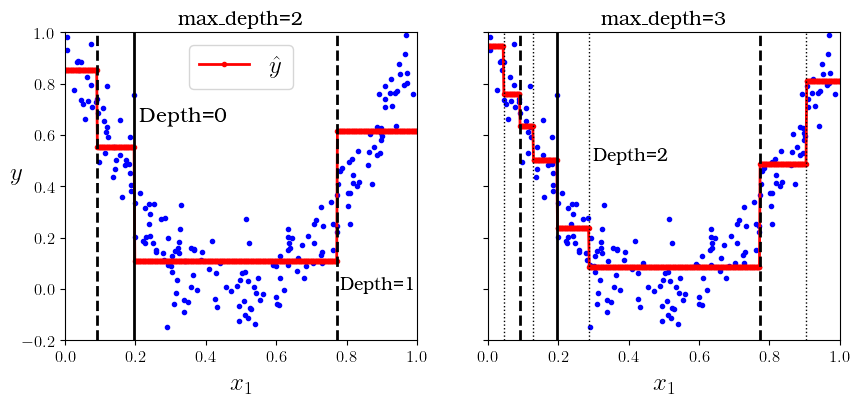
\includegraphics[width=.9\textwidth]{02_figures/fig6_5_partspace_geron09.png}
    \caption{Prediction of two Decision tree regression models \bcitep{Geron.2019}}
    \label{fig:geron6_5}
\end{figure}

The resulting decisions for the best possible splits can be represented using binary tree, this makes decision tree highly interpretable and easy to implement. The inherent logic structure from {\tt if-then} statements means that it can handle various types of data (sparse, skewed, continuous, categorical, etc.) without the need for data pre-processing. Decision tree implicitly conducts feature selection which is a desirable trait for many modelling problems \bcitep{Kuhn.2013}.\\

However, a single decision tree suffers from overfitting when the model is unconstrained. The logical principle of {\tt if-then} statements means that decision tree will attempt to fit the training data as closely as possible. Furthermore, a single decision tree model tends to be unstable, altering the data will cause drastic changes in the structure of the tree, there exist possibilities where completely different sets of splits might be found resulting in different interpretations \bcitep{Hastie.2009,Kuhn.2013}.\\

From \Cref{fig:partitionspace}, it can be implied that each decision boundaries are orthogonal to an axis i.e. all splits are perpendicular to an axis and this form rectangular subspaces for each predicted value. If the relationship between predictors and response cannot be adequately defined by the rectangular subspaces, then tree based models will suffer from larger prediction error than other kinds of models \bcitep{Kuhn.2013}.\\

Therefore, it is necessary to regularise i.e., restrict the decision tree's freedom to grow during model training. Overfitting could be reduced by controlling how deep the tree can grow through the {\tt max\_depth} parameter. Additionally, setting the amount of minimum number of samples a leaf node has, through {\tt min\_samples\_leaf} can alleviate overfitting as well, as shown in \Cref{fig:geron6_6}. Other regularisation techniques will be discussed in \Cref{sec:hpo}.\\ 

Regularisation of decision tree will help to address the overfitting issues and improve the robustness of the model, this may result in better generalisation capability. Nonetheless, in order to attain significant improvements in the performance of decision tree model, it is necessary to seek alternative solutions.\\

\begin{figure}
    \centering
        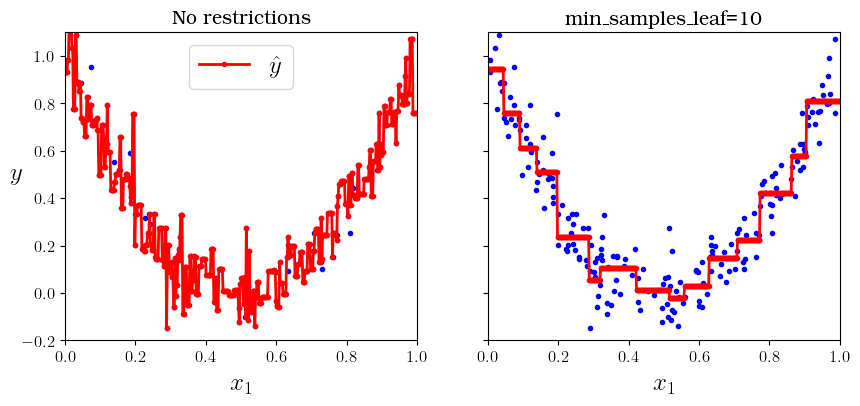
\includegraphics[width=.9\textwidth]{02_figures/fig6_6_paramdepth_geron09.png}
        \caption{Regularising a Decision Tree regressor \bcitep{Geron.2019}}
        \label{fig:geron6_6}
\end{figure}

\subsection{Random Forest}\label{sec:rf_theo}

Ensemble learning is one of the possible solutions to improve the performance of DT regressors. The main idea of ensemble learning is combining the strengths of a collection of simpler base models \bcitep{Hastie.2009}. The algorithm, involving the creation of bootstrap samples, random selection of splitting feature and aggregation of the prediction is termed by \bcitet{Breiman.2001} as \textbf{\emph{Random Forest}}. It involves combination of multiple learning algorithms, known as weak learners. In random forest, each of these learners are individual decision tree.\\

The most common ensemble methods are \emph{boosting} and \emph{bagging}. In boosting, the learner evolves over time, where successive trees are dependent on the earlier trees. In bagging (short for \emph{bootstrap aggregating}) each tree is trained using bootstrap sample of the training set i.e. this means that a sample of the training dataset is randomly selected and allowed to appear more than once\footnote{This sampling technique is referred to as sampling \emph{with} replacement}. Each model in the ensemble then generates a prediction from the bootstrapped sample and the predictions are aggregated across the learners \bcitep{TinKamHo.1995,Breiman.2001}.\\

The performance of bagging can be further improved by reducing correlation between trees i.e. de-correlating trees. This can be achieved by adding randomness during tree construction process. \bcitet{Dietterich.2000} introduced the idea of random split selection, which means that a feature $k$ will be selected from a random subset of feature. From this random subset, the assignment of the feature for the parent node follows the CART algorithm described in \Cref{eqn:costfun}. Further randomness is added by exploiting the instability of single decision tree mentioned in \Cref{sec:dt_theo}.\\

The methodology introduced in random forest address the tendency of decision tree to overfit and the issue of lack of robustness. De-correlating trees means that each learner is independent of each other, and the combination of many independent, strong learners yields an improvement in error rates i.e. reduction in variance and robustness against noisy response. It is also proven by \bcitet{Breiman.2001} that random forest cannot overfit, that means growing more trees should not affect the performance of random forest, albeit with a greater computational burden. Both \bcitet{Kuhn.2013} and \bcitet{Hastie.2009} reported that remarkable prediction results can be obtained without extensive tuning of tree parameter. \\

However, random forest loses the benefit of interpretability of tree-based model. Due to ensemble nature of random forest, it is not possible to gain an understanding between the feature and the prediction. Nevertheless, it is still possible to quantify the impact of each feature in the ensemble \bcitep{Kuhn.2013}\footnote{Known as feature importances in \scikit/}. Random forest also tends to perform poorly with small number of samples \bcitep{Hastie.2009}. Nevertheless, it is possible to traverse through a single tree to see the path taken to reach the predicted value.\\

\subsection{Extra-Trees (Extremely Randomised Trees)}\label{sec:et_theo}

Extra-trees (Extremely Randomised Trees) is introduced by \bcitet{Geurts.2006} to further randomise random forest and further de-correlate the trees in the forest. Unlike random forest, which selects the optimal split by selecting the best feature among randomly selected subset of features, Extra-trees selects a split at random. Extra-trees also does not bootstrap the sample\footnote{This sampling technique is referred to as sampling \emph{without} replacement} and uses the whole training dataset. The random selection of split means that it saves computational power and the increase in variance caused by tree de-correlation can be countered by increasing the number of trees in the ensemble.\\ 

\pagebreak

\section{AIS Data}\label{sec:ais_theo}

\subsection{Overview of AIS}

Automatic Identification System (AIS) is an automated tracking system onboard ships to automatically transmit information about the ship to other ships and coastal authorities, AIS was developed to avoid ship collision accidents. As part of the revised new chapter V of SOLAS\footnote{International Convention for the Safety of Lives at Sea} regulation, International Maritime Organization (IMO) requires all international voyage ships of 300 gross tonnage (GT) and upwards, cargo ships with 500 GT not engaged on international voyage, and all passenger ships irrespective of size to be equipped of AIS class A equipment \bcitep{Yang.2019,webimo.2014}.\\

AIS uses Very High Frequency (VHF) with special protocol for communication system for information exchange between the ships. This information will be received by either ships directly, buoys, Land based AIS transceivers (T-AIS) and satellites (S-AIS). The information transmitted by AIS is distinguished into three different types. \textbf{Static information} which is entered into the AIS on installation. \textbf{Dynamic information}, which is automatically updated from the ship's sensors connected to AIS and \textbf{voyage-related information}, which might need to be manually entered and updated during the voyage. The structure of the AIS data that is relevant to this thesis is summarised in \Cref{tbl:AIS_struct}\bcitep{webimo.2014}.\\

AIS is also further differentiated by its equipment class. The classification is based on the reporting interval and the type of information that is conveyed. \textbf{Class A} autonomously report their position within 2-10 seconds interval, depending on the state of ship's movement. The reporting interval is less frequent at 3 minutes, When the ship is at anchor or moored and moving slower than 3 knots. Class A AIS is also capable of sending safety related information, meteorological and hydrological data, electronic broadcast to mariners and marine safety messages. \textbf{Class B} reports at longer interval and at a lower power. They can only receive safety related messages, not send them. \bcitep{Rakke2016,webimo.2014}\\

\begin{table}[h!]
    \footnotesize
    \centering
    % \resizebox {\textwidth}{!}
    {\begin{tabular}{ p{0.2\linewidth} p{0.65\linewidth}  }
    \hline
    \textbf{Information Item} & \textbf{Description} \\
    \hline
    \multicolumn{2}{l}{\textbf{Static}}\\
    \hline
    MMSI & MMSI number of vessel\\
    Callsign & Callsign of vessel \\
    Name & Name of the vessel \\
    IMO & IMO number of the vessel \\
    Length & Length of vessel \\
    Width & Width of vessel \\
    Ship Type & Describes the AIS ship type of this vessel \\
    \hline
    \multicolumn{2}{l}{\textbf{Dynamic}}\\
    \hline
    Ship's position & Automatically updated from position sensor connected to AIS. Longitude and Latitude.\\
    Position time stamp in UTC & Automatically updated from ship's main position sensor. Format: DD\slash MM\slash YYYY HH:MM:SS\\
    Course over Ground (COG) & \emph{\textbf{If available}}, automatically updated from ship's main position sensor connected to AIS.\\  
    Speed Over Ground (SOG) & \emph{\textbf{If available}}, automatically updated from the position sensor connected to AIS.\\
    Heading & Automatically updated from the ship's heading sensor connected to AIS\\
    Navigational status & Navigational status information has to be manually entered by the Officer on Watch (OOW) and changed as necessary. For example : ``\emph{underway by engines}'',``\emph{engaged in fishing}'',``\emph{at anchor}''.\\
    Rate of Turn (ROT) & \emph{\textbf{If available}}, Automatically updated from the ship's ROT sensor or derived from
    the gyro.\\
    \hline
    \multicolumn{2}{l}{\textbf{Voyage Related}}\\
    \hline
    Ship's draught & To be manually entered at the start of the voyage using the
    maximum draft for the voyage and amended as required \\
    Cargo Type & Type of (hazardous) cargo from AIS message.\\
    Destination and ETA & To be manually entered at the start of the voyage and kept up to
    date as necessary.\\
    \hline
    \end{tabular}}
\caption{Structure of AIS data \bcitep{webimo.2014}}\label{tbl:AIS_struct}
\end{table}

\pagebreak

It is also stated by \bcitet{Yang.2019} that AIS data can be combined with data from other databases to provide additional information such as:\\

\begin{itemize}
    \setlength\itemsep{0em}
    \item Port to port average speed, the voyage time can be calculated from the time stamps reported by AIS data; the voyage distance can be found from corresponding navigation distance tables.
    \item Cargo weight which can be estimated from draught and ship size.
    \item Technical ship specification from fleet database which can be derived from IMO number.
    \item Port to port bunker consumption which can be estimated based on the speed, technical ship specification and distance between two ports.
\end{itemize}

\subsection{Speed Correction}\label{sec:SOG_corr}

The speed that is shown in AIS is the speed over ground (SOG). However, the ship actual speed i.e. speed through water (STW) will be required to calculate the bunker fuel consumption. Therefore, the SOG will need to be corrected for STW. This correction is performed by considering the current speed $V_c$ and the direction of the current $\gamma$ \emph{with respect to True North}. In principle, STW will be greater than SOG, when the current is moving against the current as the ship tries to compensate for the current to maintain the SOG. Whereas, the STW will be greater than the SOG when the current is moving in the same direction of the ship movement. \\

To calculate the correction, this study will adopt the methodology proposed by Kim et al. \bcitep{Kim.2020b} and Yang et al. \bcitep{Yang.2020}. The $x$ and $y$ component of SOG can be obtained through vector decomposition using the ship's heading angle $\alpha$ \emph{with respect to True North}. Similar vector decomposition is also performed for current speed $V_{\text{C}}$, it is resolved with current direction $\gamma$ \emph{with respect to True North}:\\

\begin{equation}\label{eqn:sogx}
    v_{\text{G}}^x = v_{\text{G}}\cdot\sin(\alpha)   
\end{equation}
\begin{equation}\label{eqn:sogy}
    v_{\text{G}}^y = v_{\text{G}}\cdot\cos(\alpha)   
\end{equation} 
\begin{equation}\label{eqn:vcurrx}
     v_{\text{C}}^x = v_{\text{C}}\cdot\sin(\gamma)   
\end{equation}
\begin{equation}\label{eqn:vcurry}
    v_{\text{C}}^y = v_{\text{C}}\cdot\cos(\gamma)   
\end{equation}

Then the resulting equation to determine STW,$v_{\text{S}}$, including the current compensation, is given by:\\

\begin{equation}\label{eqn:stwx}
    v_{\text{S}}^x = v_{\text{G}}^x - v_{\text{C}}^x    
\end{equation}
\begin{equation}\label{eqn:stwy}
    v_{\text{S}}^y = v_{\text{G}}^y - v_{\text{C}}^y      
\end{equation}
\begin{equation}\label{eqn:stwabs}
    v_{\text{S}} = \sqrt{(v_{\text{S}}^x)^2 + (v_{\text{S}}^y)^2} 
\end{equation}

\subsection{Source of error in AIS}\label{sec:AIS_error}

Errors and inaccuracies may still exist in AIS data. The main source of errors is caused by data that requires manual entry such as static information and voyage related information which include estimated time of arrival (ETA) and draught. There exist cases where MMSI is shared by different ships even though it is supposed to be unique. The data that is automatically connected by sensors can be erroneous, this may happen when the sensors are faulty or when it is not properly installed \bcitep{Yang.2019}. Therefore, data preprocessing of AIS data is an important step to ensure correct representation of the ship state.\\    

\section{Weather data}\label{sec:weather_theo}

During voyage, a vessel may encounter winds and waves from different directions with varying degree of magnitude. This may affect the vessel's path taken during the voyage and also ship performance such as speed and engine power, furthermore it may also affect the seakeeping capability of a vessel \bcitep{Molland.2011}. It is important to consider different weather conditions to ensure accurate and precise estimation of required engine power by the vessel. With that in mind, the discussion in this section will focus on definition of wind and wave effects, as well as the relation between some of these parameters. \\  

\subsection{Definitions of weather parameters}\label{sec:weather_definition}

\subsubsection*{Wind Waves and Swell}

\textbf{Wind Waves} are also known as wind sea, wind waves are irregular and short-crested waves generated by local wind. \textbf{Swell} are waves that travel outside the wave generation area and are no longer the result of wind, they take on regular and long-crested appearance \bcitep{Holthuijsen.2007}

\subsubsection*{Significant Wave Height, $H_{1/3}$}

It is defined as the mean of the highest one-third of waves in the wave record. The distribution of wave heights can be represented by probability density function. Hence, the term ``highest one-third of waves'' here means the region of wave heights that belong in the upper one-third of a probability density function, this is illustrated in \Cref{fig:wavestats}. From this distribution, the relation between significant wave height $H_{1/3}$, the highest ten percent of waves $H_{10}$, maximum wave height $H_{max}$ and average wave height $\overline{H}$ can be summarised as follows \bcitep{bretschneider.1965,Holthuijsen.2007}: 
\begin{equation}\label{eqn:Hsig_mean}
    \overline{H} = 0.625\cdot H_{1/3}
\end{equation}
\begin{equation}\label{eqn:Hsig_Hten}
    H_{10} = 2.03\cdot \overline{H} = 1.27\cdot H_{1/3} 
\end{equation}
\begin{equation}\label{eqn:Hsig_max}
    H_{\text{max}} = 2 \cdot H_{1/3} 
\end{equation} 

Additionally, \bcitet{BitnerGregersen.2005} and \bcitet{Nielsen.2020} described the relation between the significant wave height, wind wave height and swell height through following equation:

\begin{equation}\label{eqn:H_sig_root}
    H_{1/3} = \sqrt{(H_{\text{swell}})^2 + (H_{\text{windwave}})^2} 
\end{equation}

\begin{figure}[h]
    \centering
        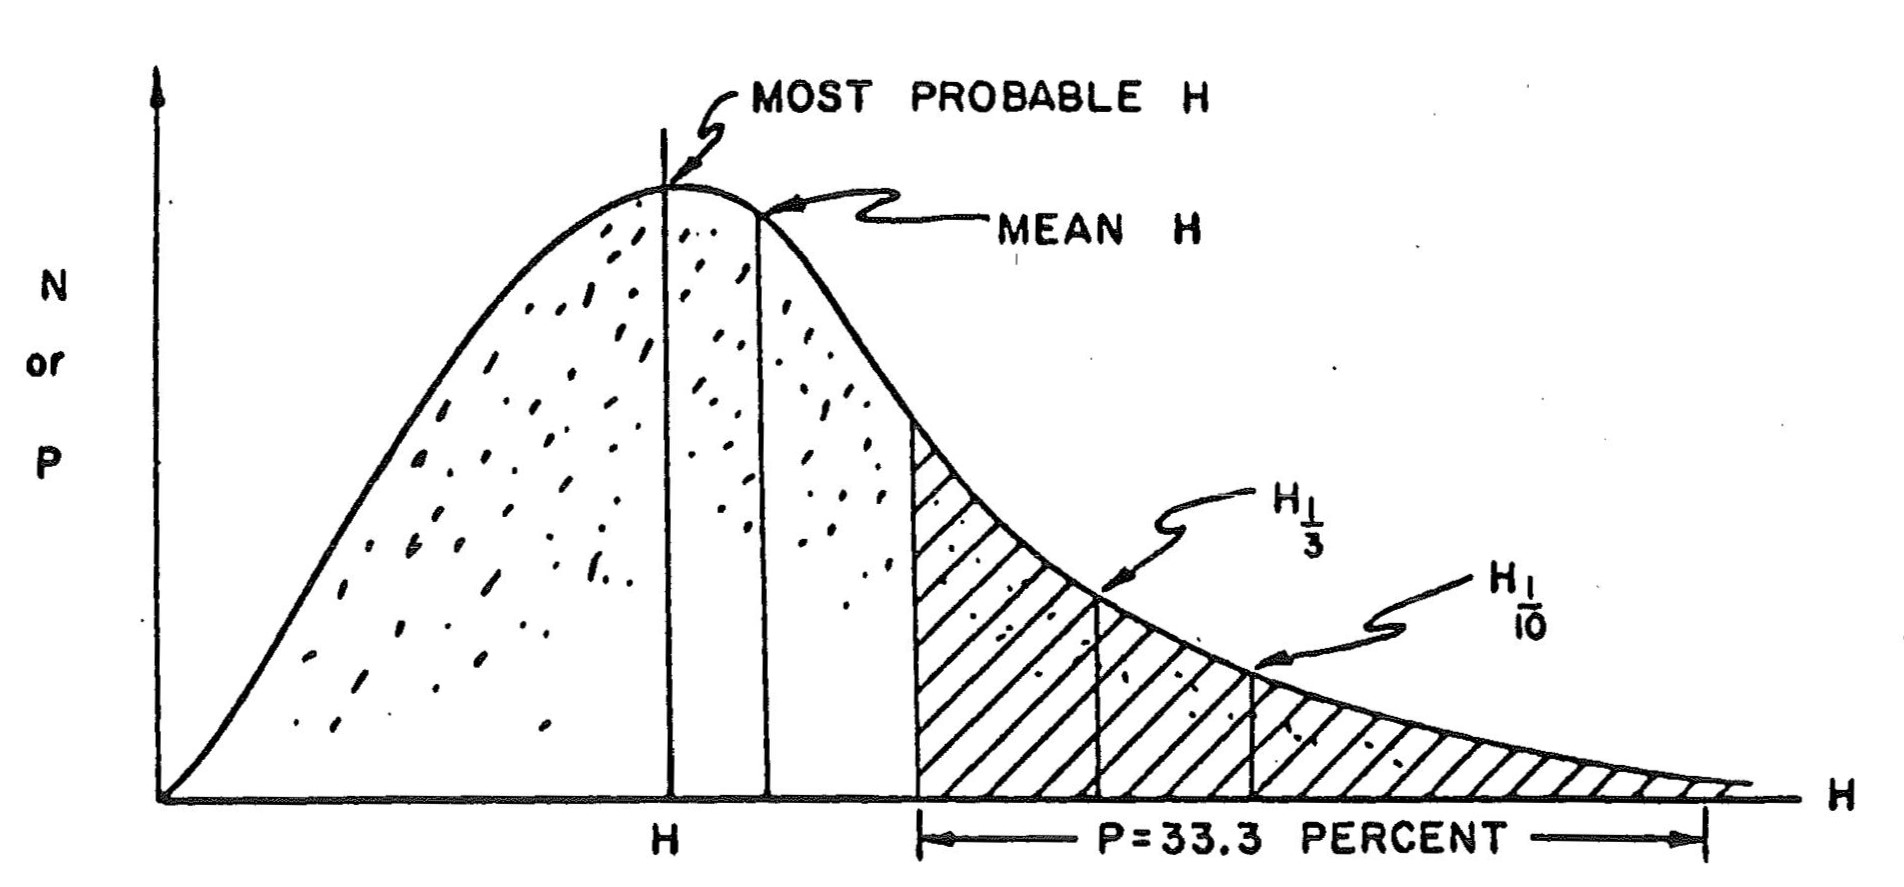
\includegraphics[width=.75\textwidth]{02_figures/Bretschneider_1965_wavedist.jpg}
        \caption{Statistical distribution of wave heights \bcitep{bretschneider.1965}}
        \label{fig:wavestats}
\end{figure}

\pagebreak

\subsubsection*{Wave Period}

Defined as the time interval between the start and the end of a wave. Some characteristics of wave period can be derived to define wave spectrum.

\subsubsection*{Wave Spectrum}

The most important form in which ocean waves are described. Wave spectrum characterises all possible observations of the waves which include wave heights, frequencies i.e. period and wave direction. For example, \bcitet{BitnerGregersen.2005} stated that the state of the sea can be described through the significant height $H_{1/3}$ and spectral peak period $\text{T}_p$ with the help of Torsethaugen peak, given the spectral peak period of fully developed sea $\text{T}_f$ and constant $a_f = 6.6$  \bcitep{K.Torsethaugen.2004}. 

\begin{equation}\label{eqn:T_p_spectralpeak}
    \text{T}_p = a_f\cdot H_{1/3}
\end{equation}
\begin{equation}
    \label{eqn:H_s_and_Tp}
    \text{Sea State (SS)} = 
    \begin{cases}
        \begin{aligned}
            &\text{Swell dominated}  &&\text{\textbf{if}} \quad \text{T}_p > \text{T}_f \\ 
            &\text{Wind sea dominated} && \text{\textbf{if}} \quad \text{T}_p \leqslant \text{T}_f 
        \end{aligned}     
    \end{cases} 
\end{equation}

\pagebreak

\section{General concept of ship propulsion}\label{sec:power_calc}

A ship's bunker fuel consumption in actual operating conditions is affected by several factors including the operating parameter of the ship's engine, propeller efficiency, and encountered resistance by the ship. Furthermore, a ship's propulsion power is correlated to the sailing speed (SOG) and meteorological conditions \bcitep{XiaoLang.2020}. Therefore, in addition to the calm water resistance $R_{CALM}$, the additional resistance caused by wind $R_{AA}$ and wave $R_{AW}$ should be considered to estimate the total resistance of the ship $R_{TOTAL}$. The power needed to propel a ship forward at a given ship STW $v_S$, to overcome $R_{TOTAL}$ is defined as \textbf{effective power $P_e$}:

\begin{equation}\label{eqn:R_tot}
    R_{TOTAL} = R_{TOTAL} + R_{AW} + R_{AA} 
\end{equation}

\begin{equation}\label{eqn:P_e}
    P_e = R_{TOTAL}\cdot v_{S}
\end{equation}

The effective power $P_e$ is transmitted through the shaft connected to the main engine of the ship which generates power to rotate the propeller of the ship, which is termed as \textbf{brake power of the engine, $P_b$}. The brake power can be calculated through effective power by considering the \textbf{shaft efficiency $\eta_s$, hull efficiency $\eta_h$, relative rotative efficiency $\eta_r$ and open water efficiency $\eta_o$}:

\begin{equation}\label{eqn:P_b}
    P_b = \frac{P_e}{\eta_s\cdot\eta_h\cdot\eta_r\cdot\eta_o}
\end{equation}

The bunker fuel consumption can then be calculated by multiplying the brake power $P_b$ with the Specific Fuel Oil Consumption (SFOC) and the operation time:

\begin{equation}\label{eqn:FOC}
    FOC = P_b\cdot SFOC\cdot \mathcal{T}_{operation} 
\end{equation}

\subsection{Ship dimensions and form coefficients}\label{sec:Ship_design_param}

\subsubsection*{Principal Dimension of a vessel}

The summary of important ship dimensions and parameters are shown in \Cref{fig:biran14_shipside} and \Cref{fig:biran14_shipfront} \bcitep{Biran.2014}:

\begin{figure}[ht]
    \centering
    \begin{minipage}[b]{0.5\linewidth}
        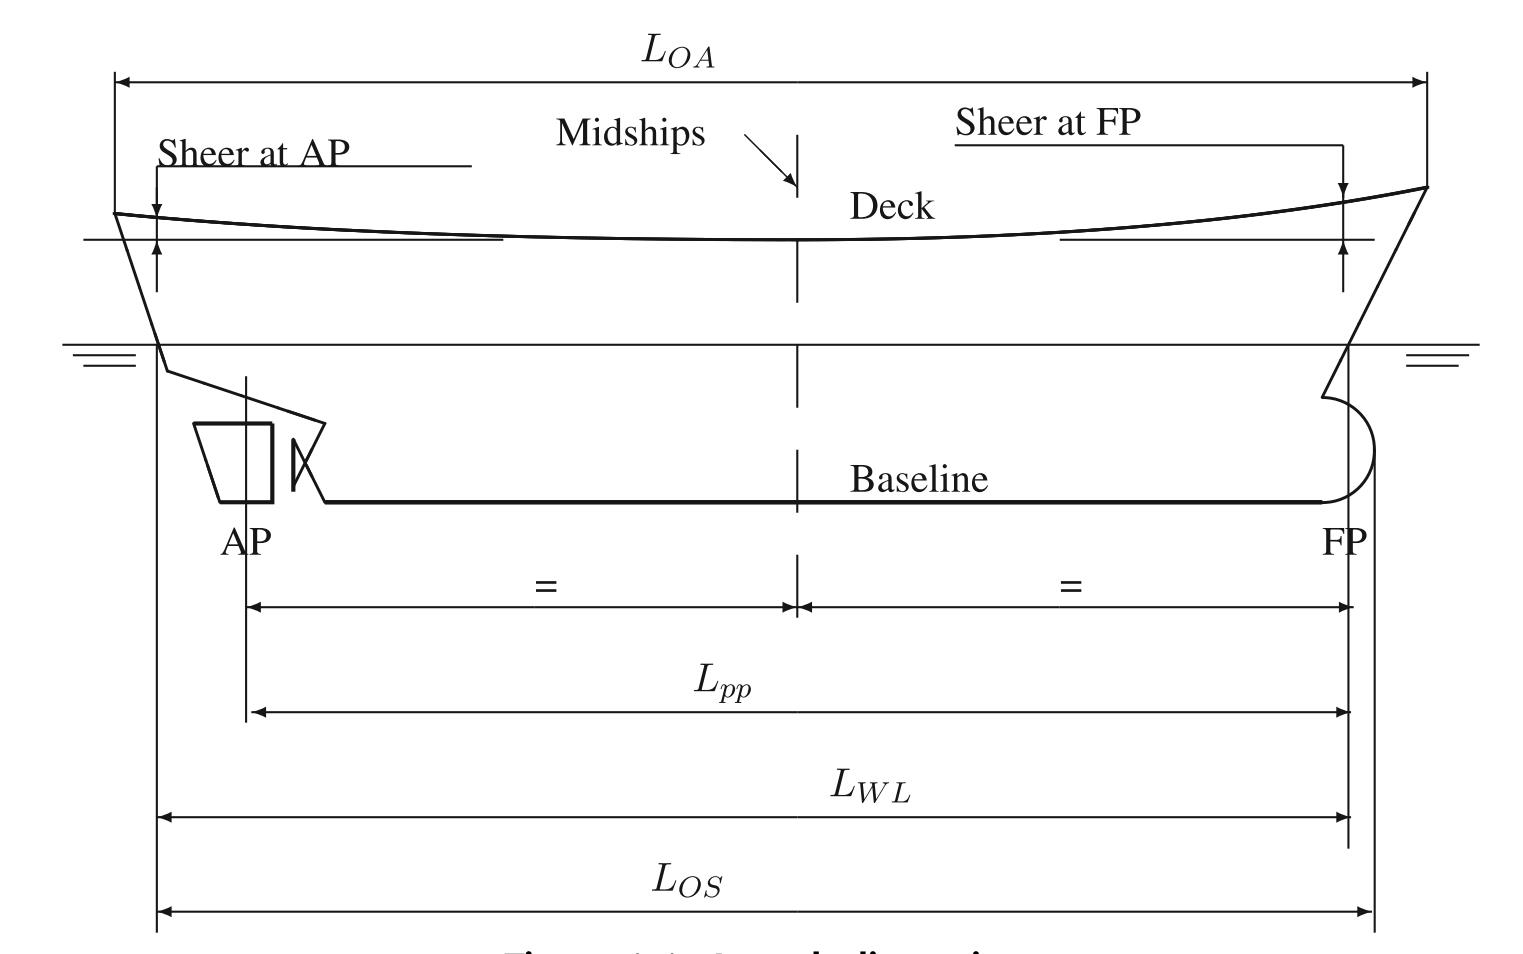
\includegraphics[width=\linewidth]{02_figures/biran14_shipside .jpg}
        \caption{Side view of a vessel}
        \label{fig:biran14_shipside}
    \end{minipage}
    \hfill
    \begin{minipage}[b]{0.45\linewidth}
        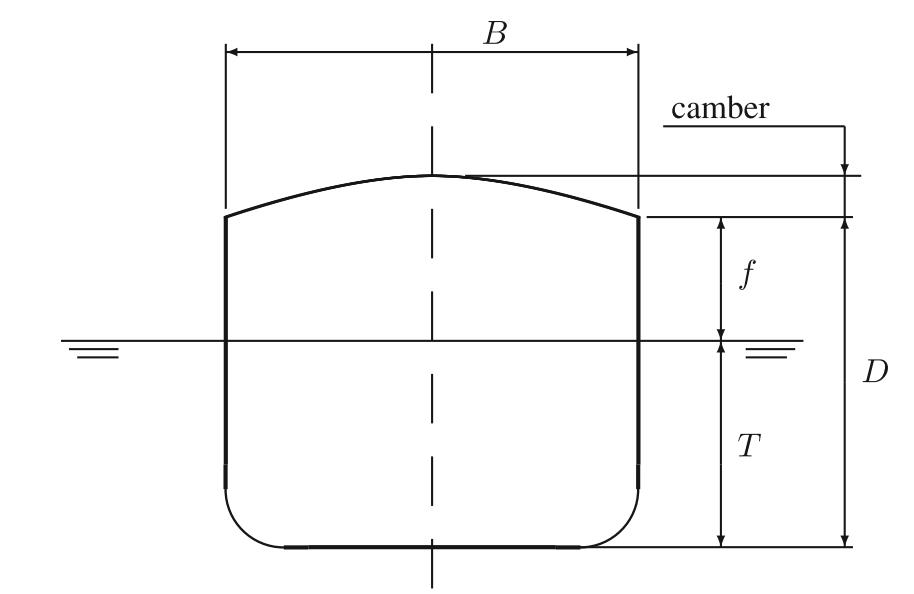
\includegraphics[width=\linewidth]{02_figures/biran14_frontship .jpg}
        \caption{Front view of a vessel}
        \label{fig:biran14_shipfront}
    \end{minipage}
\end{figure}

The outer surface of the ship is usually not uniform as not all plates have the same thickness, Therefore the hull surface is measured with respect to the inner surface of the plating which is termed as \emph{moulded surface} of the hull. All dimensions measured to this surface are defined as \emph{moulded} dimensions whereas dimensions measured to the outer surface of the hull or of an appendage are qualified as \emph{extreme} dimensions \bcitep{Biran.2014}.

\subsubsection*{Coefficients of form}

The form coefficients are non-dimensional numbers required to classify the hulls and to find relationships between forms and their properties, the summary of some important form coefficients are summarised in \Cref{fig:man_formcoeff} 

\begin{figure}[ht]
    \centering
        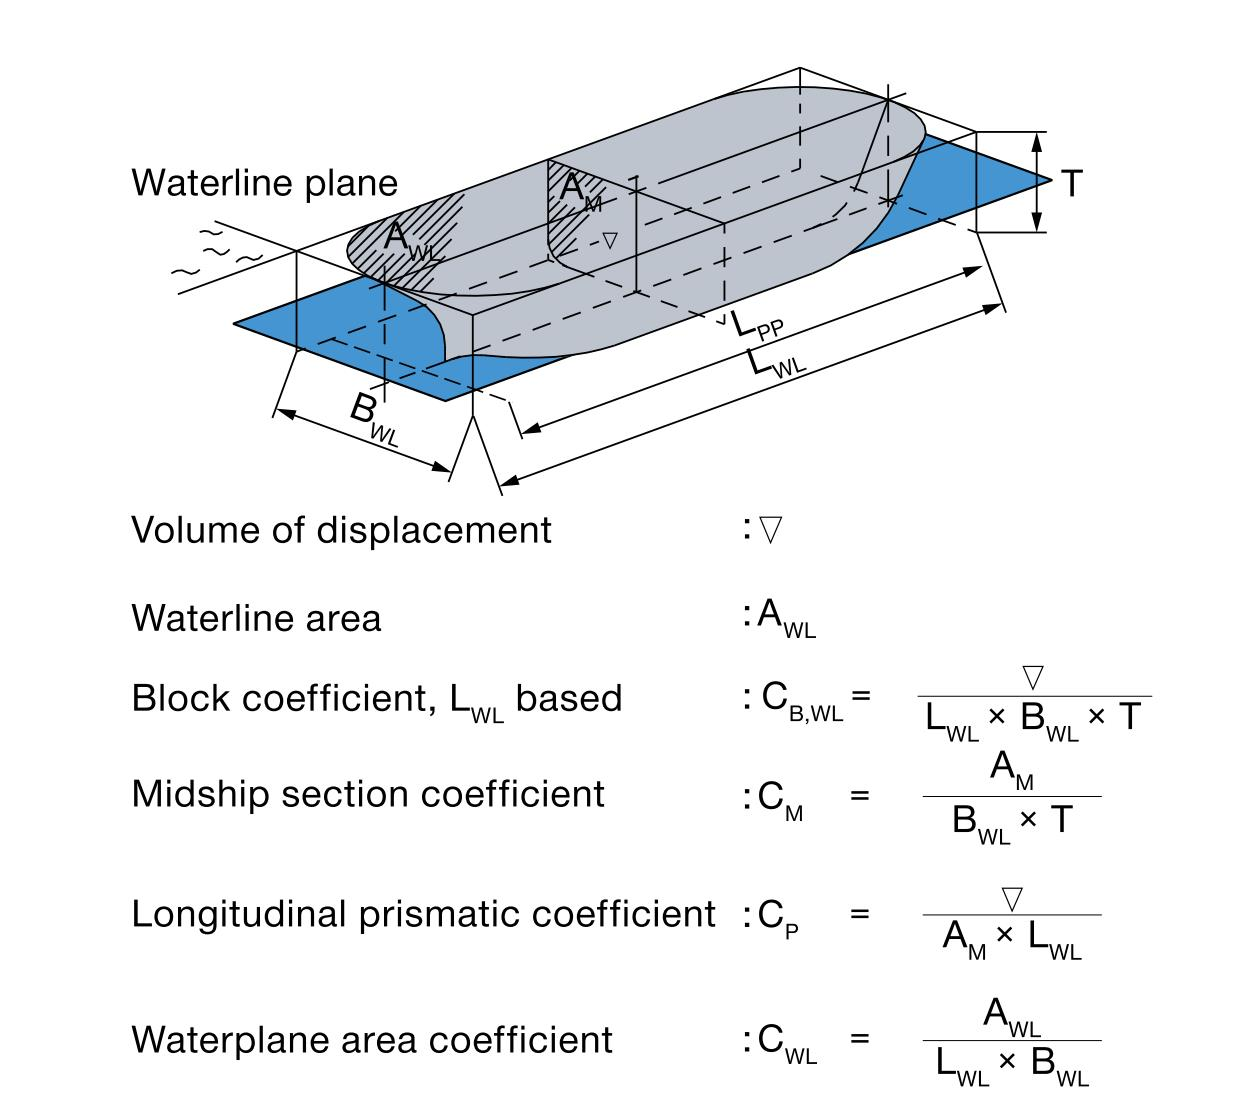
\includegraphics[width=.6\textwidth]{02_figures/man11_shipcoeff.jpg}
        \caption{Form coefficients \bcitep{Diesel.2011}}
        \label{fig:man_formcoeff}
\end{figure}

\subsubsection*{Block Coefficient}
\textbf{Block Coefficient $C_B$} is defined as the ratio of moulded displacement volume to the volume of parallelepiped (rectangular block) with dimensions $L,B$ and $T$. Alternatively, \bcitet{Schneekluth.1998} provided an estimation of the value using the Froude number within the range of $0.15 < Fr < 0.32$

\begin{equation}
    \label{eqn:Cb_Schneekluth}
    C_b = -4.22 + 27.8\sqrt{Fr} - 39.1Fr + 46.6Fr^3
\end{equation}

The Froude number $Fr$ is defined with the following equation:

\begin{equation}
    \label{eqn:Froude_Number}
    Fr = \frac{v}{\sqrt{gL_{WL}}}
\end{equation}

\subsubsection*{Midship Coefficient}
\textbf{Midship Coefficient $C_M$} is defined as the ratio of the midship-section area $A_M$ to the product of breadth and draught, $BT$. According to \bcitet{Schneekluth.1998}, changing $C_M$ value will have an effect on separation resistance and wave resistance. \bcitet{jensen1994moderne} presented a method based on regression equation on a graph to calculate $C_M$:  

\begin{equation}
    \label{eqn:CM_jensen}
    C_M = \frac{1}{1+(1-C_B)^{3.5}}
\end{equation}

\begin{figure}[ht]
    \centering
        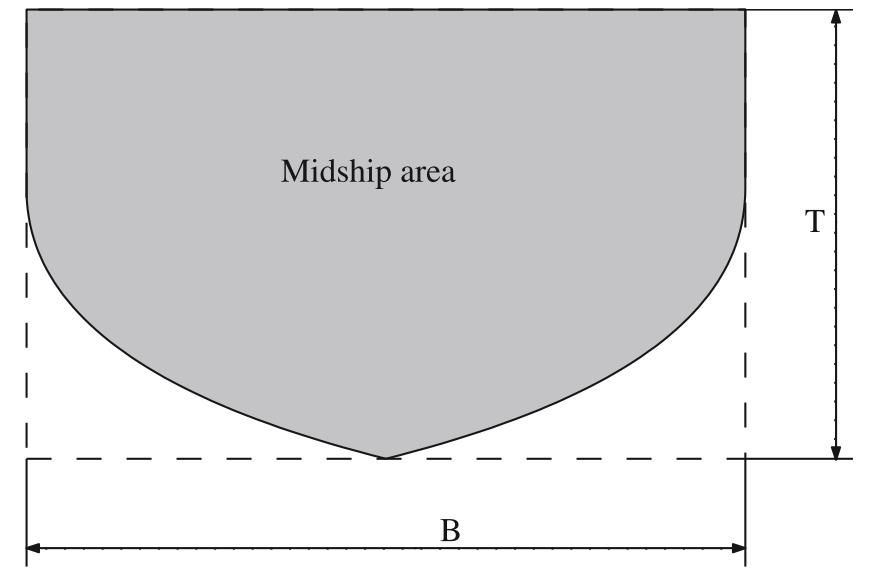
\includegraphics[width=.4\textwidth]{02_figures/biran14_cm.jpg}
        \caption{Definition of $C_M$ \bcitep{Biran.2014}}
        \label{fig:biran_cm}
\end{figure}

\subsubsection*{Prismatic Coefficient}

\textbf{Prismatic Coefficient $C_P$} is defined as the ratio of moulded displacement volume\footnote{In some notations it is denoted as $\nabla$} $V$. It is an indicator on how much of a cylinder with constant section $A_M$ and length $L$ is filled with submerged hull as shown in \Cref{fig:biran_cp}.

\begin{equation}
    \label{eqn:cp_ratio}
    C_P = \frac{C_B}{C_M}
\end{equation}

\begin{figure}[ht]
    \centering
        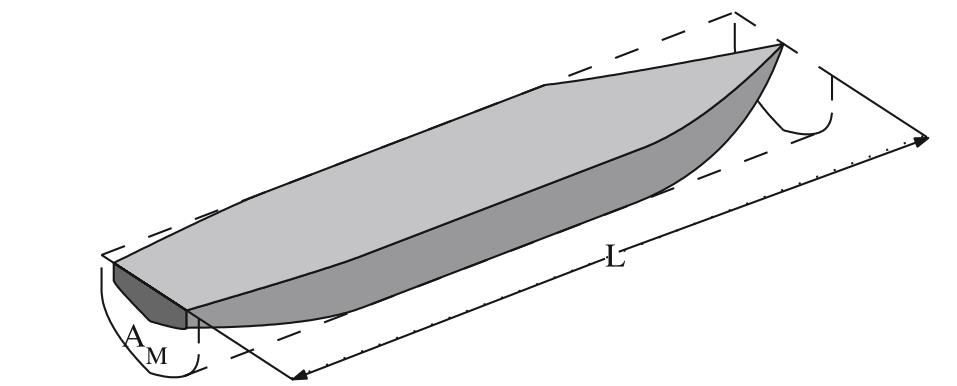
\includegraphics[width=.5\textwidth]{02_figures/biran14_cp.jpg}
        \caption{Definition of $C_P$ \bcitep{Biran.2014}}
        \label{fig:biran_cp}
\end{figure}

\pagebreak

\subsubsection*{Waterplane area coefficient}

\textbf{Waterplane area coefficient $C_{WP}$} is defined as the ratio between the ship's waterline area $A_{W}$ and the product of $L$ and $B$. In ship design, $C_{WP}$ significantly impacts resistance and stability \bcitep{Schneekluth.1998}. \bcitet{Diesel.2011} approximated that $C_{WP}$ is 0.10 higher than $C_B$, alternatively \bcitet{Schneekluth.1998} provided the following formulation for $C_{WP}$:

\begin{equation}
    \label{eqn:cwp_Schneekluth}
    C_{WP} = \frac{1+2C_B}{3}
\end{equation}

\begin{figure}[ht]
    \centering
        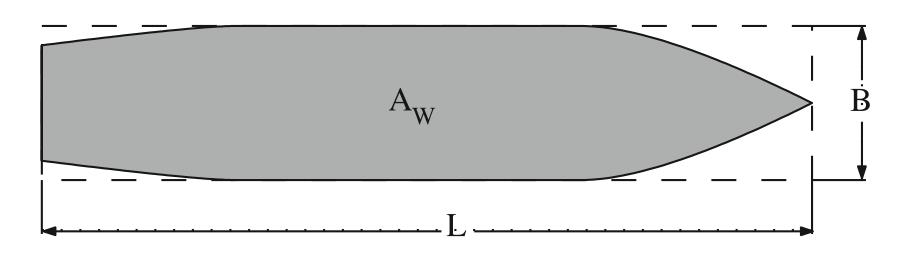
\includegraphics[width=.5\textwidth]{02_figures/biran14_cwp.jpg}
        \caption{Definition of $C_{WP}$ \bcitep{Biran.2014}}
        \label{fig:biran_cwp}
\end{figure}

\subsection{Holtrop \& Mennen's Method}\label{sec:holtrop_mennen_calc}

This power prediction method was applied in the late 1970s and early 1980s by J. Holtrop and G.G.J Mennen and it was based on regression analysis of vast model tests and trial data of MARIN, the model basin in Wageningen, The Netherlands. This gives Holtrop-Mennen method a wide applicability range and the only method that adopted the use of the ITTC form factor $k$. The resistances in this method are calculated as dimensional force. Furthermore, the method also gives estimates of hull-propeller interaction, thrust deduction, full-scale wake fraction and relative rotative efficiency \bcitep{Birk.2019}. 

\begin{table}[ht]
    \footnotesize
    \centering
    % \resizebox {\textwidth}{!}
    {\begin{tabular}{ p{0.45\linewidth} p{0.08\linewidth} p{0.38\linewidth}  }
    \hline
    \textbf{Parameter} & \textbf{Symbol} & \textbf{Remarks} \\
    \hline
    Required Parameters&&\\
    \hline
    Length in waterline & $L_{WL}$\\
    Moulded breadth & $B$ \\
    Moulded mean draught & $T$ & typically $T = \frac{1}{2}(T_A+T_F)$ \\
    Moulded draught at aft perpendicular & $T_A$ & \\ 
    Moulded draught at forward perpendicular & $T_F$\\
    Volumetric displacement (molded) & $V$ & alternatively use the block \mbox{coefficient} as $C_B = V/BTL_{WL}$\\
    Prismatic coefficient (based on $L_{WL}$) & $C_P$ \\
    Midship section coefficient & $C_M$ & or use $C_M=C_B/C_P$ \\
    Waterplane area coefficient & $C_{WP}$ & may have to be estimated in early design stages\\
    Longitudinal Centre of buoyancy & $\ell_{CB}$ &positive forward; with respect to $L_{WL}/2$ in percent of $L_{WL}$\\
    Area of ship and cargo above waterline & $A_V$ & projected in direction of $v_S$\\
    Immersed transom area & $A_T$ & measured at rest\\
    Transverse area of bulbous bow & $A_{BT}$ & Measured at forward perpendicular \\
    Height of centre $A_{BT}$ above basis & $h_B$ & has to be smaller than $0.6T_F$ \\
    Propeller Diameter & $D$ \\
    Propeller expanded area ratio & $A_E/A_0$ \\
    Stern shape parameter & $C_{stern}$ \\
    \hline
    Optional Parameters&&\\
    \hline
    Wetted surface (hull) & $S$\\
    Wetted Surface of appendages & $S_{App}$ & bilge keels, stabiliser fins, etc.\\
    Half angle of waterline entrance & $i_E$ \\
    Diameter of bow thruster tunnel & $d_{TH}$ \\
    \hline
    \end{tabular}}
\caption{Required and optional input parameters for Holtrop \& Mennen's method according to \bcitet{Birk.2019}}
\label{tbl:holtrop_params}
\end{table}

\subsubsection*{Application Range}

The publication from \bcitet{Holtrop.1978,Holtrop.1982,Holtrop.1984} does not provide explicit information regarding the application range of the method. However, from the experience of \bcitet{Birk.2019}, reasonable estimates from the method can be achieved for the following conditions: \\

\begin{equation}
    \label{eqn:holtrop_cond}
    % \begin{multlined}
    \begin{gathered}
        Fr \leqslant 0.45 \\
        0.55 \leqslant C_p \leqslant 0.85 \\
        3.9 \leqslant \frac{L}{B} \leqslant 9.5
    \end{gathered}
    % \end{multlined}
\end{equation}

\subsubsection{Calm water resistance}\label{sec:Calm_Resistance}

The calm water resistance $R_{CALM}$ is broken down into several components and can be approximated using the following relation:

\begin{equation}\label{eqn:R_calm}
    R_{CALM} = R_F(1+k_1) + R_{APP} + R_W + R_B + R_{TR} + R_A
\end{equation}

\subsubsection*{Frictional Resistance $R_F$}

\textbf{$R_F$} is calculated using the ITTC-1957 frictional resistance correlation line $C_F$ as the basis of a representation of a resistance plate with a wetted surface area $S$ of bare hull. 

\begin{equation}\label{eqn:R_f}
    R_F = \frac{1}{2}\rho v_{S}^2 S C_F 
\end{equation}

The frictional coefficient $C_F$ can be calculated through the Reynold number $Re$ for a given ship speed $v_{S}$ and kinematic viscosity $\nu$:

\begin{equation}\label{eqn:C_F}
    C_F = \frac{0.075}{[\log_{10}(Re)-2]^2} \quad \textbf{where} \quad Re = \frac{v_{S}L_{WL}}{\nu}
\end{equation}

If not known, then the wetted surface area of bare hull $S$ can be estimated by the following formula:

\begin{equation}\label{eqn:S_bh}
    S = c_{23}L_{WL}(2T+B)\sqrt{C_M}+2.38\frac{A_{BT}}{C_B}
\end{equation}

with the factor $c_{23}$ given as :

\begin{equation}\label{eqn:c_23}
    c_{23} = \biggl[0.453 + 0.4425C_B - 0.2862C_M - 0.003467\frac{B}{T} + 0.3696C_{WP} \biggr]
\end{equation}

The flat plate resistance is subsequently adjusted by including a form factor $k$ during the calculation of total resistance. The constant $c_{14}$ must be determined first to calculate form factor $k$, which serves the purpose of capturing the impact of the aft body shape.   

\begin{equation}\label{eqn:c_14}
    c_{14} = 1.0 + 0.011C_{stern} \quad \textbf{with} \quad \begin{array}{l c}
        \text{Aft body shape} & C_{stern}\\
        \hline
        \text{Pram with gondola} & -25 \\
        \text{V-shaped sections} & -10 \\
        \text{Normal sections} & 0 \\
        \text{U-shaped sections} & +10 \\
        \hline
    \end{array}
\end{equation}

To complete the required input for the calculation of $(1+k_1)$, the length of run $L_R$ can be estimated from the following equation:

\begin{equation}\label{eqn:L_R}
    L_R = L_{WL}(\frac{1-C_P+0.06C_P\ell_{CB}}{4C_P-1})
\end{equation}

The formula by \bcitet{Guldhammer.1974} can be used if $\ell_{CB}$ is not known:

\begin{equation}
    \label{eqn:lcb}
    \ell_{CB} = -(0.44Fr - 0.094)
\end{equation}

Then, the form factor $(1+k_1)$ can be determined with the constant $c_{14}$, the length of run $L_R$ and input values from \Cref{tbl:holtrop_params}.

\begin{multline}\label{eqn:1+k1}
    1+k_1 = 0.93 + 0.487118c_{14}\Biggl[ \Biggl(\frac{B}{L_{WL}}\Biggr)^{1.06806}  \Biggl(\frac{T}{L_{WL}}\Biggr)^{0.46106} \\ 
    \Biggl(\frac{L_{WL}}{L_R}\Biggr)^{0.121563} \Biggl(\frac{L_{WL}}{V}\Biggr)^{0.36486} (1-C_p)^{-0.604247} \Biggr] 
\end{multline}

\subsubsection*{Appendage Resistance}

An appendage is defined as addition to the main part or main structure of a vessel \bcitep{Molland.2011}. Examples of appendages include rudders, shaft brackets, skeg and bilge keels. The form factors associated with these appendages, denoted as $k_{2_i}$ are presented in \Cref{tbl:k2i_values}. In practice, reasonable estimates can be made based on these form factors, as model tests are not the most suitable method for accurately quantifying appendage resistance. Furthermore, effects of appendages are typically considered as a whole and not as individual unit \bcitep{Birk.2019}.\\

\begin{table}[ht]
    \footnotesize
    \centering
    {\begin{tabular}{ p{0.6\linewidth} c}
    \hline
    Appendage & $k_{2_i}$ value \\
    \hline
    rudder behind skeg & $0.2-0.5$ \\
    rudder behind stern & $0.5$ \\
    twin screw rudder (slender) & $1.5$ \\
    twin screw rudder (thick) & $2.5$ \\
    shaft brackets & $2.0-4.0$ \\
    skeg & $0.5-1.0$ \\
    strut bossing & $2.0-3.0$ \\
    hull bossing & $1.0$ \\
    exposed shafts (angle with buttocks about 10 degrees) & $1.0$ \\
    exposed shafts (angle with buttocks about 20 degrees) & $4.0$ \\
    stabiliser fins & $1.8$ \\
    dome & $1.7$ \\
    bilge keels & $0.4$ \\ 
    \hline
    \end{tabular}}
\caption{Approximate values for appendage form factors $k_{2_i}$}\label{tbl:k2i_values}
\end{table}

The equivalent form factor for multiple appendages, $(1+k_{2_i})_{eq}$ is given by:

\begin{equation}\label{eqn:k2eq}
    (1+k_{2_i})_{eq} = \frac{\sum_i(1+k_{2_i})S_{APP_i}}{\sum_iS_{APP_i}}
\end{equation}

If bow thruster is present, the resistance due to the bow thruster tunnel $R_{TH}$ can be obtained through:

\begin{equation}\label{eqn:R_th}
    R_{TH} = \rho v_S^2 \pi \d_{TH}^2 C_{D_{TH}} \quad \textbf{where} \quad C_{D_{TH}} = 0.003 + 0.003 \Biggl( \frac{10{d_{TH}}}{t} - 1 \Biggr) 
\end{equation}

The coefficient $C_{D_{TH}}$ defines the drag coefficient for the tunnel, and it ranges between $0.003$ and $0.012$. Smaller values indicate thrusters which are in the cylindrical part of bulbous bow. The coefficient can also be estimated using the equation by \bcitet{Hollenbach.1999} in \Cref{eqn:R_th}.\\

With that, the appendage resistance $R_{APP}$ can be calculated using:

\begin{equation}\label{eqn:R_app}
    R_{APP} = \frac{1}{2}\rho v_S^2 (1+k_{2_i})_{eq} C_F \sum_i S_{APP_i} + \sum R_{TH}
\end{equation}

\subsubsection*{Wave Resistance}

The estimation of wave resistance $R_W$ is dependent on Froude number $Fr$, and it is subdivided into three categories.\footnote{Considering the length of the equations, only the scenario where $Fr \leqslant 0.4$ will be thoroughly examined in this thesis. The formulations of $R_W$ for other ranges of Froude number can be referenced in the studies by \bcitet{Holtrop.1984} and \bcitet{Birk.2019}}:

\begin{equation}
    \label{eqn:case_Rw}
    R_W(Fr) = 
    \begin{cases}
        \begin{aligned}
        &R_{W_a}(Fr) && \textbf{if} \quad Fr \leqslant 0.4 \\
        &\text{Interpolation} && \textbf{if} \quad 0.4 < Fr \leqslant 0.55 \\
        &R_{W_b}(Fr) && \textbf{if} \quad Fr > 0.5 \\
    \end{aligned}
    \end{cases}
\end{equation}

The wave resistance for $R_{W_a}(Fr)$ can be calculated using:

\begin{equation}\label{eqn:R_w_low}
    R_{W_a}(Fr) = c_1 c_2 c_5 \rho g V  \exp \biggl[ m_1 Fr^d + m_4 \cos(\lambda Fr ^{-2}) \biggr]
\end{equation}

And consequently for $R_{W_b}(Fr)$:

\begin{equation}\label{eqn:R_w_high}
    R_{W_b}(Fr) = c_{17} c_2 c_5 \rho g V  \exp \biggl[ m_3 Fr^d + m_4 \cos(\lambda Fr ^{-2}) \biggr]
\end{equation}

The remaining range of Froude number between $0.4 < Fr \leqslant 0.55 $ are calculated by mean of interpolation between equation \Cref{eqn:R_w_low} and \Cref{eqn:R_w_high}. However, this range of Froude number is considered uneconomical and ship does not operate in this speed range for extended durations \bcitep{Birk.2019}.

\begin{equation}\label{eqn:R_w_mid}
    R_W(Fr) = R_{W_a}(0.4) + \frac{20Fr-0.8}{3} \biggl[ R_{W_b}(0.55) - R_{W_a}(0.4)\biggr]
\end{equation}

To compute each of the constants in \Cref{eqn:R_w_low}, The following equations are presented, note that the calculations for the \textbf{$\cos (\lambda Fr^{-2})$} are in \textbf{Radians}:

\begin{equation}\label{eqn:c_7}
    c_7 = \begin{cases}
        \begin{aligned}
        &0.229577\biggl(\frac{B}{L_{WL}} \biggr)^\frac{1}{3}  &&\textbf{if} \quad \frac{B}{L_{WL}} \leqslant 0.11 \\
        &\frac{B}{L_{WL}}  &&\textbf{if}  \quad 0.11 < B/L_{WL} \leqslant 0.25\\
        &0.5 - 0.0625\frac{L_{WL}}{B}  &&\textbf{if}  \quad B/L_{WL}>0.25 
        \end{aligned} 
    \end{cases}
\end{equation}

\begin{equation}\label{eqn:c_1}
    c_1 = 2223105c_7^{3.78613}\biggl( \frac{T}{B}\biggr)^{1.07961}(90-i_e)^{1.37565}
\end{equation}

$i_E$ is defined as the half angle of the waterline entrance and the estimation can be calculated by:

\begin{equation}\label{eqn:i_e}
    i_E = 1+89 e^{a}
\end{equation}

and $a$ can be obtained through:

\begin{multline}\label{eqn:a_const_ie}
    a = -\biggl[ \biggl(\frac{L_{WL}}{B}\biggr)^{0.80856} \biggl(1 - C_{WP}\biggr)^{0.30484} \biggl[1 - C_P - 0.0225\ell_{CB}\biggr]^{0.6367} \\
    \biggl(\frac{L_R}{B}\biggr)^{0.34574} \biggl(\frac{100V}{L_{WL}^3}\biggr)^{0.16302} \biggr]
\end{multline}

\begin{equation}\label{eqn:c3}
    c_3 = 0.56 \frac{A_{BT}}{\left[BT\left(0.31 \sqrt{A_{BT}} + T_F + h_B\right)\right]}
\end{equation}

\begin{equation}\label{eqn:c2}
    c_2 = e^{(-1.89\sqrt{c_3})}
\end{equation}

\begin{equation}
    \label{eqn:c15}
    c_{15} =
    \begin{cases}
        \begin{aligned}
            & -1.69385 && \textbf{if} \quad \frac{L_{WL}^2}{V} \leqslant 512 \\
            & -1.69385 + \frac{\frac{L_{WL}}{V^{(1/3)}}-8}{2.36}&& \textbf{if} \quad 512 < \frac{L_{WL}^2}{V} \leqslant 1726.91 \\
            & 0 && \textbf{if} \quad \frac{L_{WL}^2}{V} > 1726.91
        \end{aligned}
    \end{cases}
\end{equation}

\begin{equation}
    \label{eqn:c16}
    c_{16} = 
    \begin{cases}
        \begin{aligned}
            & 8.07981C_P - 13.8673C_P^2 + 6.984338C_P^3 && \textbf{if} \quad C_P \leqslant 0.8 \\
            & 1.73014 - 0.7067C_P && \textbf{if} \quad C_P > 0.8
        \end{aligned}
    \end{cases}
\end{equation}

\begin{equation}
    \label{eqn:d}
    d = -0.9
\end{equation}

\begin{equation}
    \label{eqn:lambda}
    \lambda = 
    \begin{cases}
        \begin{aligned}
            &1.446C_P - 0.03\frac{L_{WL}}{B} && \textbf{if} \quad \frac{L_{WL}}{B} \leqslant 12 \\
            &1.446C_P - 0.36 && \textbf{if} \quad \frac{L_{WL}}{B} > 12 \\
        \end{aligned}
    \end{cases}
\end{equation}

\begin{equation}
    \label{eqn:m1}
    m_1 = 0.0140407C_P - 0.03\frac{L_{WL}}{B} - 1.75254\frac{V^{(1/3)}}{L_{WL}} - 4.79323\frac{B}{L_{WL}} - c{16}
\end{equation}

\begin{equation}
    \label{eqn:m4}
    m_4 = 0.4 c_{15} \exp{(-0.034Fr^{-3.29})}
\end{equation}

\subsubsection*{Resistance of bulbous bow}

The approximation of the resistance due to bulbous bow $R_B$ can be obtained through the immersion Froude number $F_{r_i}$ for the bulbous bow and the constant $P_B$ which is a measure of the emergence of the bow: 

\begin{equation}
    \label{Fr_immersion}
    Fr_i = \frac{v_S}{\sqrt{g(T_F-h_b-0.25 \sqrt{A_{BT}})+0.15v_S^2}}
\end{equation}

\begin{equation}
    \label{Pb}
    P_B = 0.56 \frac{\sqrt{A_{BT}}}{T_F-1.5h_B+h_F}
\end{equation}

\begin{equation}
    \label{eqn:Rbulb}
    R_B = 0.11 \rho g (\sqrt{A_{BT}})^3 \frac{Fr_{i}^3}{1+Fr_{i}^2}e^{(-3.0P_B^-2)}
\end{equation}

\begin{figure}[ht]
    \centering
    \begin{minipage}[b]{0.45\linewidth}
        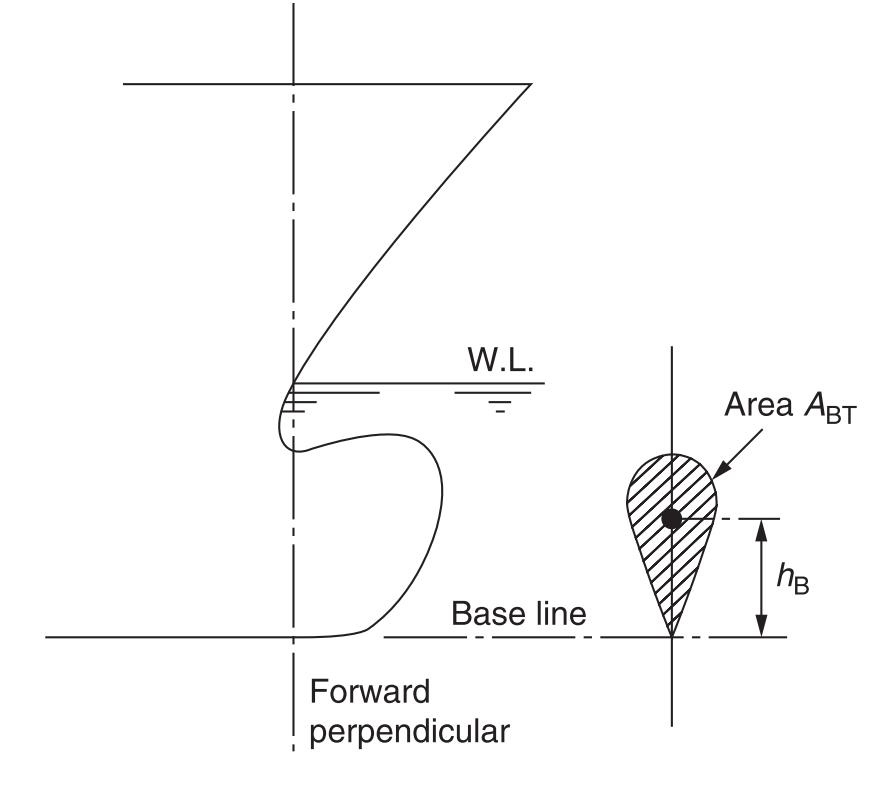
\includegraphics[width=\linewidth]{02_figures/Molland11_bulb.jpg}
        \caption{Bulbous bow definition \bcitep{Molland.2011}}
        \label{fig:molland11_bow}
    \end{minipage}
    \hfill
    \begin{minipage}[b]{0.45\linewidth}
        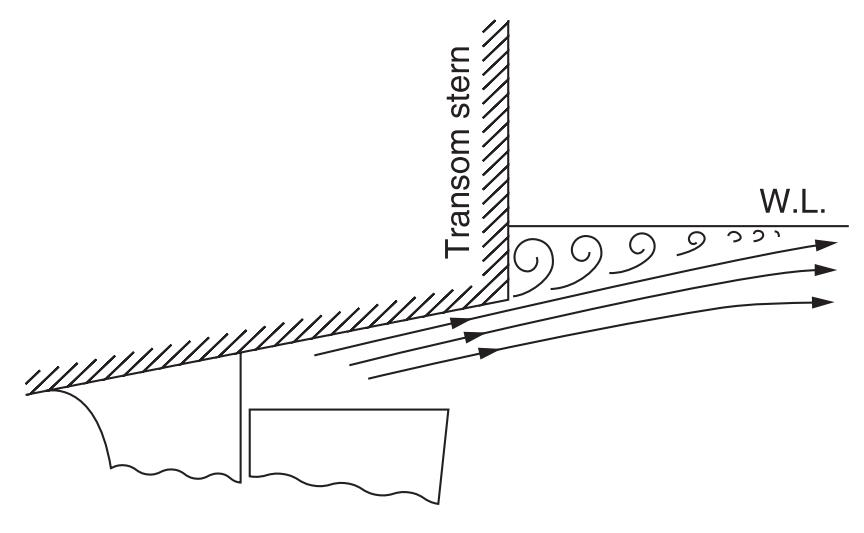
\includegraphics[width=\linewidth]{02_figures/molland11_transom.jpg}
        \caption{Flow around immersed transom stern \bcitep{Molland.2011}}
        \label{fig:molland1_transom}
    \end{minipage}
\end{figure}

\subsubsection*{(Immersed) Transom Resistance}

Transom is referred to as the flat section at the ship stern and the immersion of the transom causes pressure loss, the resulting resistance from the pressure loss are considered using the term $R_{TR}$ for immersed transom area $A_T > 0$. The transom resistance is a function of the depth Froude number $Fr_{T}$:

\begin{equation}
    \label{eqn:Fr_t}
    Fr_T = \frac{v_S}{\sqrt{\frac{2gA_T}{(B+BC_{WP})}}}
\end{equation}

The expression $A_T/(B+BC_{WP})$ is a measure for the average draught of the transom. When the average draught is smaller than the speed, there will be clean separation of the flow at transom edge and the resistance due to transom vanishes. Immersion resistance $R_{TR}$ is considered if $Fr_{T} > 5$ 

\begin{equation}
    \label{eqn:c6}
        c_6 = 
        \begin{cases}
            \begin{aligned}
              &0.2(1-0.2Fr_T) && \textbf{if} \quad Fr_T < 5 \\
              & 0 && \textbf{if} \quad Fr_T > 5  
            \end{aligned}
        \end{cases}
\end{equation}

\begin{equation}
    \label{eqn:R_transom}
    R_{TR} = \frac{1}{2}\rho v_S^2 A_T c_6
\end{equation}

\subsubsection*{Correlation allowance resistance}

The resistance term $R_A$ considers other effects that are not captured by other resistance components. 

\begin{equation}
    \label{eqn:c4}
    c_4 =
    \begin{cases}
        \begin{aligned}
            &\frac{T_F}{L_{WL}} && \textbf{if} \quad \frac{T_F}{L_{WL}} \leqslant 0.04 \\
            &0.04 && \textbf{if} \quad \frac{T_F}{L_{WL}} >0.04 
        \end{aligned}
    \end{cases}
\end{equation}

\pagebreak

The correlation allowance coefficient $C_A$ and subsequent correlation resistance is defined as:

\begin{equation}
    \label{eqn:Ca_correlation}
    C_A = 0.00546(L_{WL}+100)^{-0.16} - 0.00205 + 0.003\frac{L_{WL}}{7.5}C_{B}^4c_2(0.04-c_4)
\end{equation}

\begin{equation}
    \label{eqn:R_a}
    R_A = \frac{1}{2}\rho v_S^2 C_A (S+\sum S_{APP})
\end{equation}

\subsubsection{Added resistance due to wind}\label{sec:wind_resistance}

The magnitude of added resistance caused by wind, $R_{AA}$, is determined by the area of the ship superstructure and relative wind. Therefore, for a ship with large lateral areas above the water level, this added resistance due to wind can be significant. The estimation of added resistance due to wind in this thesis consider the method by \bcitet{Blendermann.1994}:

\begin{equation}
    \label{eqn:Raa_blendermann}
    R_{AA} = \frac{\rho_{air}}{2}u^2A_{L}CD_l \frac{\cos{(\varepsilon)}}{1-\frac{\delta}{2}(1-\frac{CD_l}{CD_t}\sin^2{(2\varepsilon)})}
\end{equation}

Where $u$ is the apparent wind velocity, $A_L$ the lateral plane area, $\varepsilon$ the apparent wind angle ($\varepsilon = 0$ in headwind). $\delta$ the cross-force parameter, and coefficients $CD_t$ and $CD_l$ the non-dimensional drag in beam wind and headwind. For given true wind velocity $u_{TW}$ and true wind angle, $\beta$, The calculation for the apparent wind $u$ and apparent wind angle $\epsilon$ is performed using the following equations:

\begin{equation}
    \label{eqn:u_AW}
    u = \sqrt{u_{\text{TW}}^2 + v_S^2 + 2 \cdot u_{\text{TW}} \cdot v_S \cdot \cos(\beta)}
\end{equation}

\begin{equation}
    \label{eqn:epsilon_AWA}
    \frac{u_{TW}}{\sin(\varepsilon)} = \frac{u}{\sin({\beta})}
\end{equation}

\begin{figure}
    \centering
        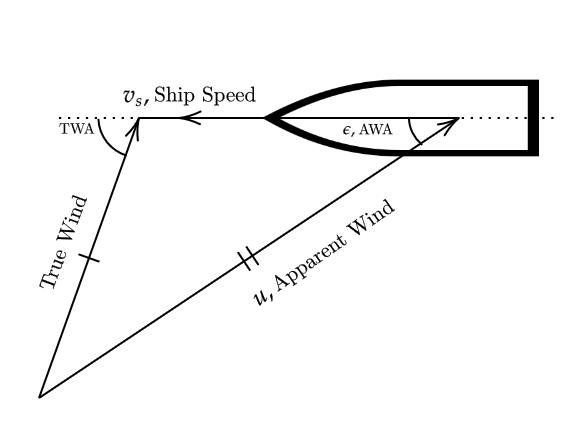
\includegraphics[width=.6\textwidth]{02_figures/AWA_TWAc.png}
        \caption{Apparent and true wind \bcitep{Knudsen.2013}}
        \label{fig:AWA_TWA}
\end{figure}

According to \bcitet{Schneekluth.1998}, maximum wind resistance is encountered when $0^\circ<\varepsilon<20^\circ$ and it is more convenient to express the longitudinal drag with respect to the frontal area $A_F$. Typical values for the constants are summarised in \Cref{tbl:BlendermannCoeff}

\begin{equation}
    \label{eqn:CDlaf}
    CD_{lAF} = CD_l \frac{A_L}{A_F}
\end{equation}

\begin{table}[ht]
    \footnotesize
    \centering
    % \resizebox {\textwidth}{!}
    {\begin{tabular}{ p{0.4\linewidth} c c c }
    \hline
    &\textbf{$CD_t$} & \textbf{$CD_{lAF}$} & \textbf{$\delta$} \\
    \hline
    Car carrier & 0.95 & 0.55 & 0.8 \\
    Cargo ship, container on deck, bridge aft & 0.85 & 0.65/0.55 & 0.40 \\
    Containership, loaded & 0.90 & 0.55 & 0.40 \\
    Ferry & 0.90 & 0.45 & 0.80\\
    LNG Tanker & 0.70 & 0.60 & 0.50 \\
    Passenger liner & 0.90 & 0.40 & 0.80 \\
    Speed boat & 0.90 & 0.55 & 0.60 \\
    Tanker, loaded & 0.70 & 0.90 & 0.40 \\
    Tanker, in ballast & 0.70 & 0.75 & 0.40 \\
    \hline        
    \end{tabular}}
\caption{Coefficients to estimate wind resistance}\label{tbl:BlendermannCoeff}
\end{table}

\pagebreak

\subsubsection{Added resistance due to wave}\label{sec:wave_resistance}

The added resistance due to wave, $R_{AW}$ is estimated using the STAWAVE-1 method recommended by \bcitet{ITTCProcedures.2014}. This method only considers waves encountered within the bow sector i.e. within $\pm 45^\circ$ off bow and does not consider wave correction for other encounters. Also, STAWAVE-1 is valid for the following condition:

\begin{equation}
    \label{eqn:stawave_cond1}
    \text {Significant wave height:} \quad H_{1/3} = 2.25\leqslant\sqrt{L_{PP}/100} 
\end{equation}

\begin{equation}
    \label{eqn:stawave1}
    R_{AWL} = \frac{1}{16}\rho g H_{1/3}^2 B \sqrt{\frac{B}{L_{BWL}}} 
\end{equation}

In which, $L_{BWL}$ is the length of bow on the water line to $95\%$ of maximum breadth.

\subsubsection{Efficiencies affecting brake power}\label{sec:Pb_efficiency}

\subsubsection*{Open water efficiency}

The open water efficiency \begin{math}\eta_O\end{math}, can be understood as the propeller working in open water conditions i.e. the propeller operates in a homogenous wake field with no hull in front of it. The curve of different propulsion devices with its respective efficiencies is summarised in the work of \bcitet{Breslin.1994}:

\begin{figure}[ht]
    \centering
        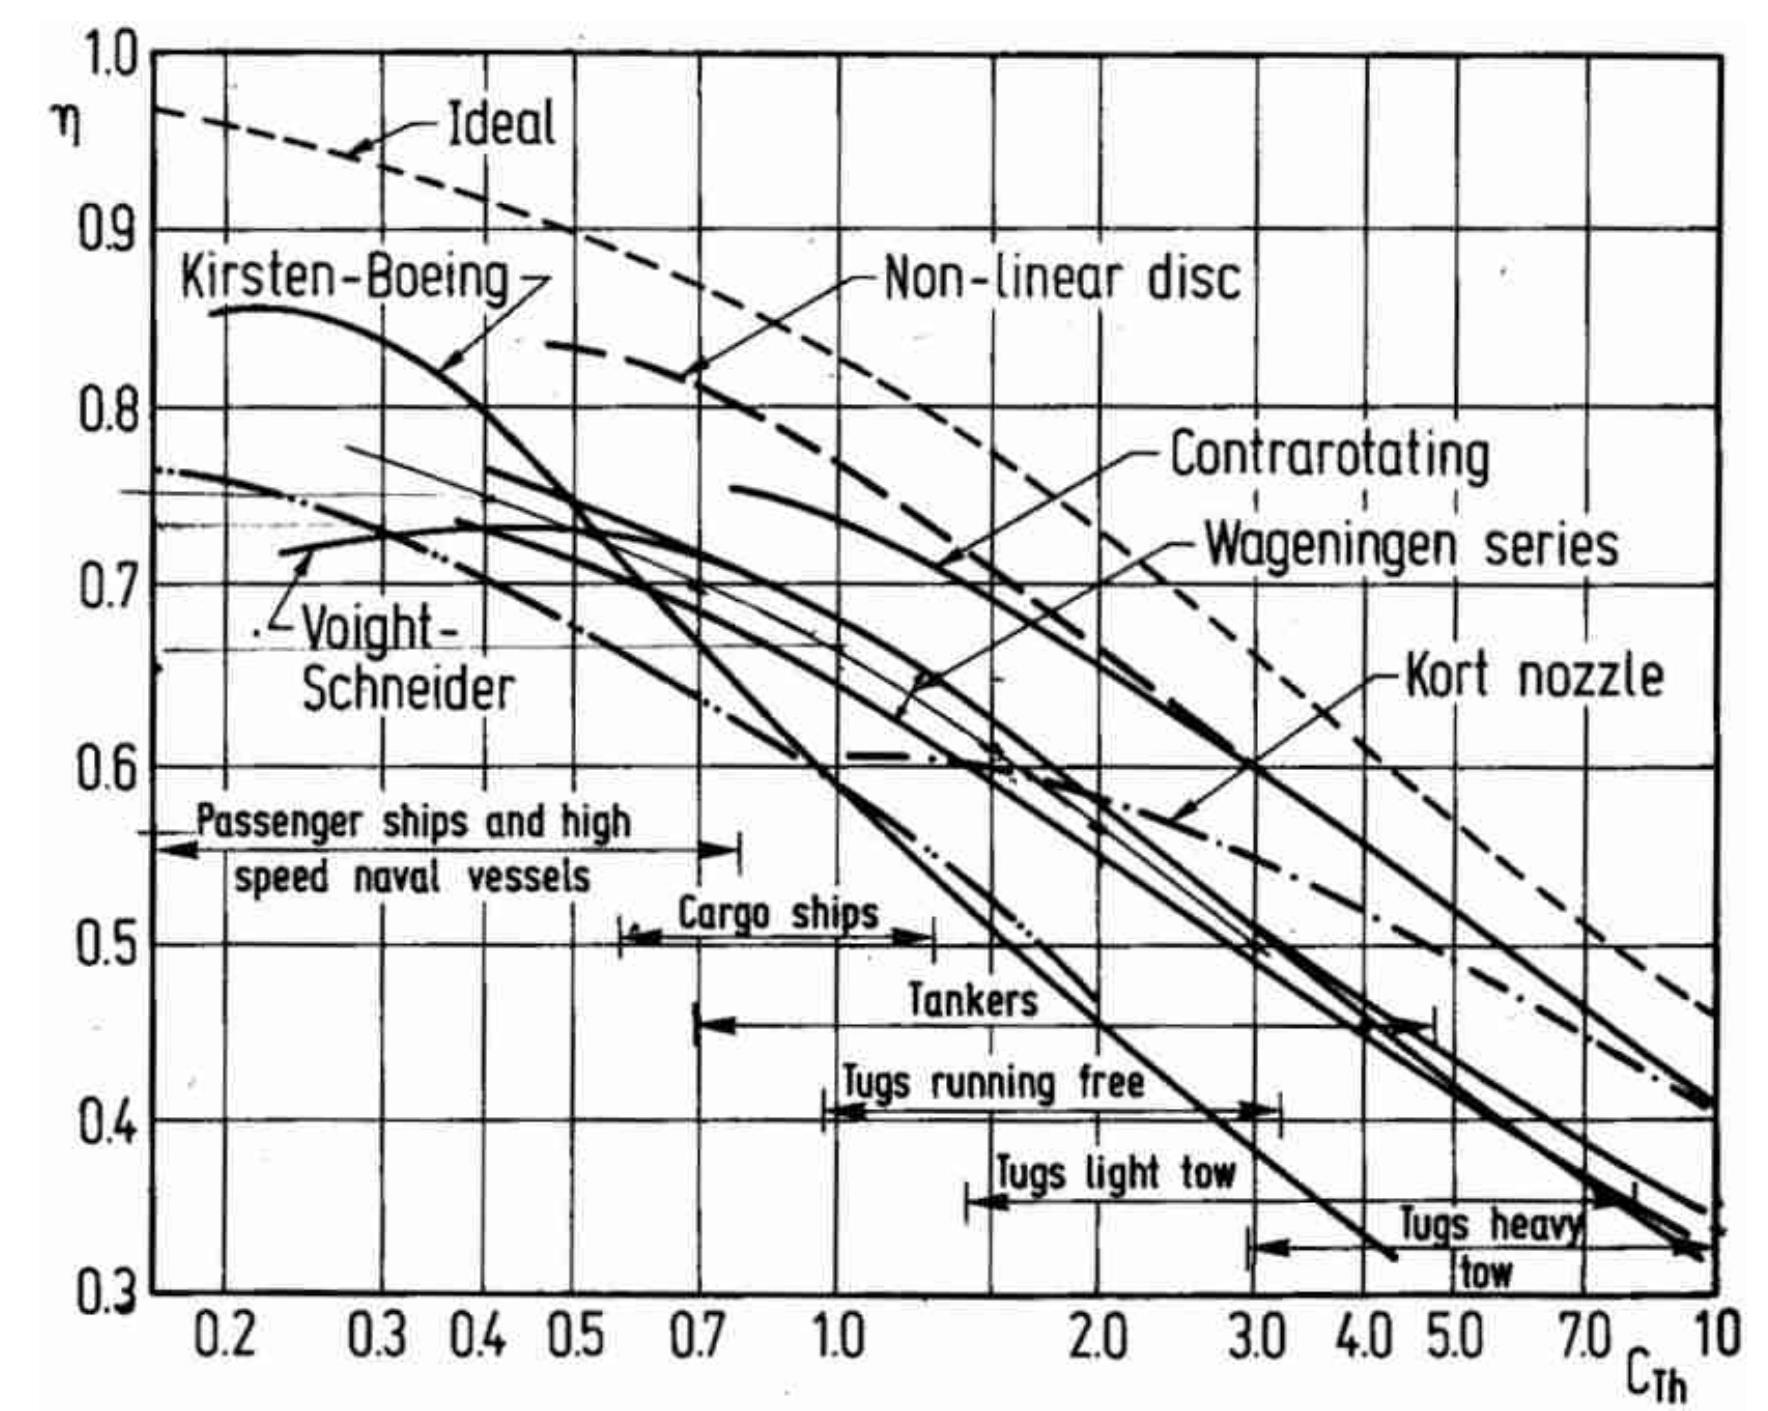
\includegraphics[width=.8\textwidth]{02_figures/Breslin94_openwater_eff.jpg}
        \caption{Efficiencies of various propulsion devices \bcitep{Breslin.1994}}
        \label{fig:breslin_open water efficiencies}
\end{figure}


\subsubsection*{Hull efficiency}

The Hull efficiency $\eta_H$ can be calculated using the following equation:

\begin{equation}
    \label{eqn:hull_eff}
    \eta_H = \frac{1 - t}{1 - w_S}
\end{equation}

The term $t$ refers to the thrust deduction fraction, which represents the thrust force required to overcome the towing resistance of the ship $R_{TOTAL}$ and the additional resistance caused by the propeller's interaction with the hull. On the other hand, the term $w_S$ corresponds to the wake fraction, characterising the influence of the ship's hull on the water flow into the propeller \bcitep{Diesel.2011,Birk.2019}. The following equations are presented for twin-screw vessels\footnote{Considering the length of the equations, the equations for single screw vessels can be obtained from \bcitet{Holtrop.1982} and \bcitet{Birk.2019}} to calculate $w_S$ and $t$.

\begin{equation}
    \label{eqn:wake_ws}
    w_S = 0.3095 C_B + 10 C_V C_B -0.23 \frac{D}{\sqrt{BT}}
\end{equation}

\begin{equation}
    \label{eqn:thrust_t}
    t = 0.325 C_B - 0.1885 \frac{D}{\sqrt{BT}}
\end{equation}

where $C_V$ is the viscous resistance coefficient, which combines all friction-related components of the resistance and the correlation resistance:

\begin{equation}
    \label{eqn:C_V}
    C_V = \frac{(1+k_1)R_F+R_{APP}+R_A}{\frac{1}{2}\rho v_S^2 (S+\sum_i S_{APP_i})}
\end{equation}

\subsubsection*{Relative rotative efficiency}

The relative rotative efficiency \begin{math} \eta_R \end{math} can be expressed by the following ratio, with $V_A$ defined as the arriving water velocity to propeller \bcitep{Diesel.2011}:

\begin{equation}
    \label{eqn: n_rot_MAN}
    \eta_R = \frac{\text{Power absorbed in open water at }V_A}{\text{Power absorbed in wake behind the ship at }V_A}
\end{equation}

According to \bcitet{Holtrop.1982}, $\eta_R$ for twin screw vessels can be estimated using the following formula, with $P/D$ defined as the propeller pitch to diameter ratio:

\begin{equation}
    \label{eqn: eta_rot_holtrop}
    \eta_R = 0.9737 + 0.111(C_P-0.0225\ell_{CB}) - 0.06325\frac{P}{D}
\end{equation}

\subsubsection*{Shaft efficiency}

The shaft efficiency \begin{math}\eta_S\end{math} is defined as the ratio between the power delivered to the propeller $P_D$ and the brake power of the main engine $P_B$, with values ranging from $\eta_S = 0.95 - 0.99$ depending on shaft design and gear configuration.


% \begin{tikzpicture}[x=0.75pt,y=0.75pt,yscale=-1,xscale=1]
%     %uncomment if require: \path (0,452); %set diagram left start at 0, and has height of 452
    
%     %Shape: Axis 2D [id:dp697661158302031] 
%     \draw  (220,297.8) -- (517.5,297.8)(249.75,80) -- (249.75,322) (510.5,292.8) -- (517.5,297.8) -- (510.5,302.8) (244.75,87) -- (249.75,80) -- (254.75,87)  ;
%     %Image [id:dp23308396965327827] 
%     \draw (245,305) node [rotate=-40.58] {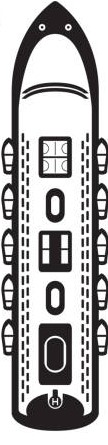
\includegraphics[width=26.87pt,height=72.39pt]{02_figures/ferry.jpg}};
% \end{tikzpicture}




% \subsection{Ship speed}


% \subsection{Modelling}



% Phased out, but might be useful

% Might be useful for multiple images !
% \begin{figure}[h]
% \centering
% \begin{minipage}[t]{.5\textwidth}
%     \centering
%     % \begin{figure}
%     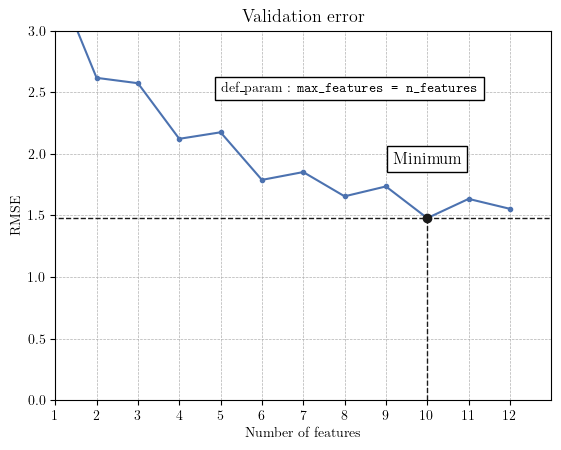
\includegraphics[width=\textwidth]{02_figures/featureserrro.png}
%     % \end{figure}
%     \captionof{figure}{Effects of number of features on RMSE}
%     \label{fig:featureserror}
% \end{minipage}%
% \begin{minipage}[t]{.5\textwidth}
%     \centering
%     % \begin{figure}
%     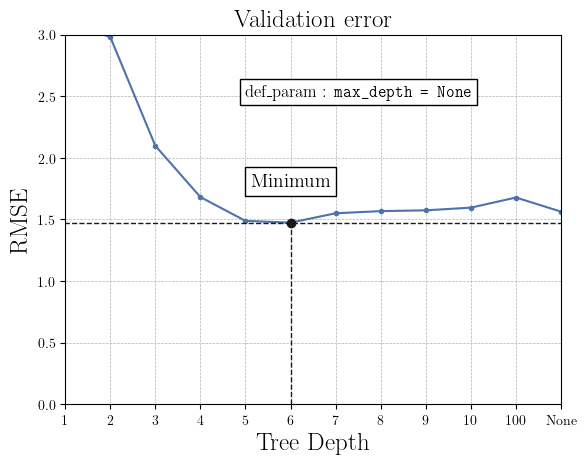
\includegraphics[width=\textwidth]{02_figures/depthError.png}
%     % \end{figure}
%     \captionof{figure}{Effects of tree depth on RMSE}
%     \label{fig:deptherror}
% \end{minipage}
% \end{figure}

% \begin{figure}[h]
%     \centering
%         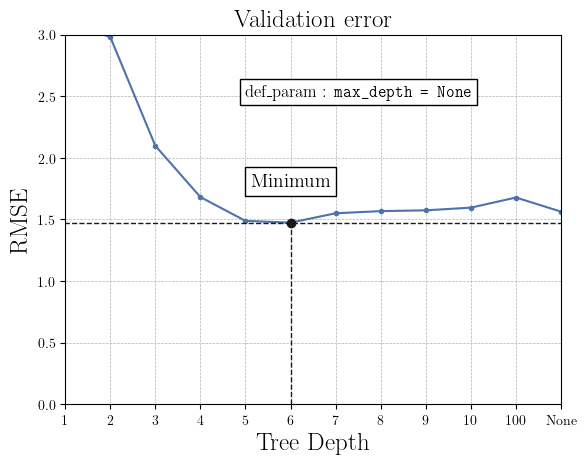
\includegraphics[width=.5\textwidth]{02_figures/depthError.png}
%         \caption{Effect of tree depth on RMSE for validation dataset}
%         \label{fig:Tree Depth Error}
% \end{figure}

% \begin{enumerate}
%     \item Possible thresholds are determined by calculating the splitting value (For example, suppose there are data points at $X = [0.2,0.4]$, then the splitting value is the value in between i.e. $t_k = 0.3$)
%     \item Calculate the mean of data points of the left and right partition space respectively, Defined by the following equation $\hat{y}_{node} = \frac{1}{m_{node}}\sum\limits_{i\in node} y ^ {(i)}$
%     \item Calculate the mean squared error (MSE) of each data points in its respective partition space. Through the equation $MSE_{node} = \sum\limits_{i\in node}(\hat{y}_{node} - y^{(i)} )^2$ 
%     \item The MSE from the respective partition space is summed.
%     \item Step $1 - 4$ is recursively repeated, until the minimum of the cost function $J(X,T_k)$, i.e. minimum MSE, is determined:
%      \begin{equation}\label{costfun}
%         J(X,t_k) = \frac{m_{left}}{m}MSE_{left} + \frac{m_{right}}{m}MSE_{right}
%         \begin{cases}
%             MSE_{node} = \sum\limits_{i\in node}(\hat{y}_{node} - y^{(i)} )^2 \\
%             \hat{y}_{node} = \frac{1}{m_{node}}\sum\limits_{i\in node} y ^ {(i)}
%         \end{cases}   
%     \end{equation}
% \end{enumerate} 
\newpage
\chapter{Research Methodology} \label{chp:method}

The methodology used to develop the grey box model will be discussed in this chapter. The grey box modelling approach in this thesis falls under the category of sequential GBM. Hence, the development process is divided into two stage. The first stage of the modelling focus on machine learning modelling i.e. BBM using tree-based model using python with help of \scikit/ \bcitep{FabianPedregosa.2011}. This includes the process of data acquisition, data preprocessing, hyperparameter optimisation and model evaluation. The training of the models utilises a fusion of T-AIS data and weather data, then, relevant features are selected to predict the SOG. These processes are visually presented in \Cref{fig:flowchart_BBM}.\\

\begin{figure}[h]
    \centering
        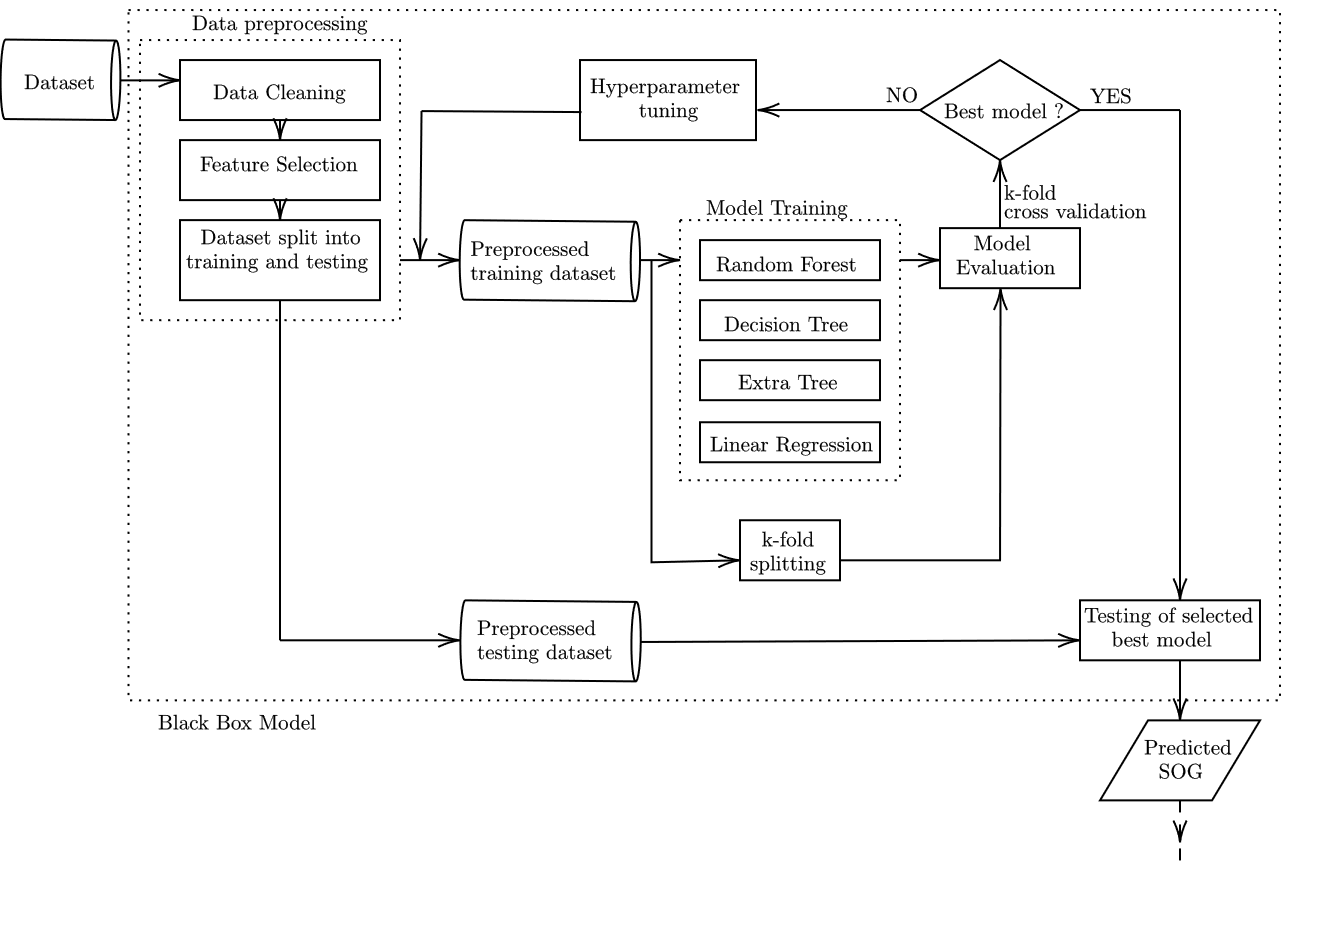
\includegraphics[width=\textwidth]{02_figures/flowmethod_BBM_alt.png}
        \caption{Scheme of proposed BBM methodology}
        \label{fig:flowchart_BBM}
\end{figure}

The second stage of the modelling focus on WBM aspect of the GBM. The predicted SOG will be fed into the WBM to predict the required brake power required to propulse the ship. The SOG will need to be first converted into STW for the resistance calculations and consequently power calculations. The framework presented in \Cref{fig:flowchart_WBM} refers is a graphical summary of \Cref{sec:power_calc}. 

\begin{figure}[h]
    \centering
        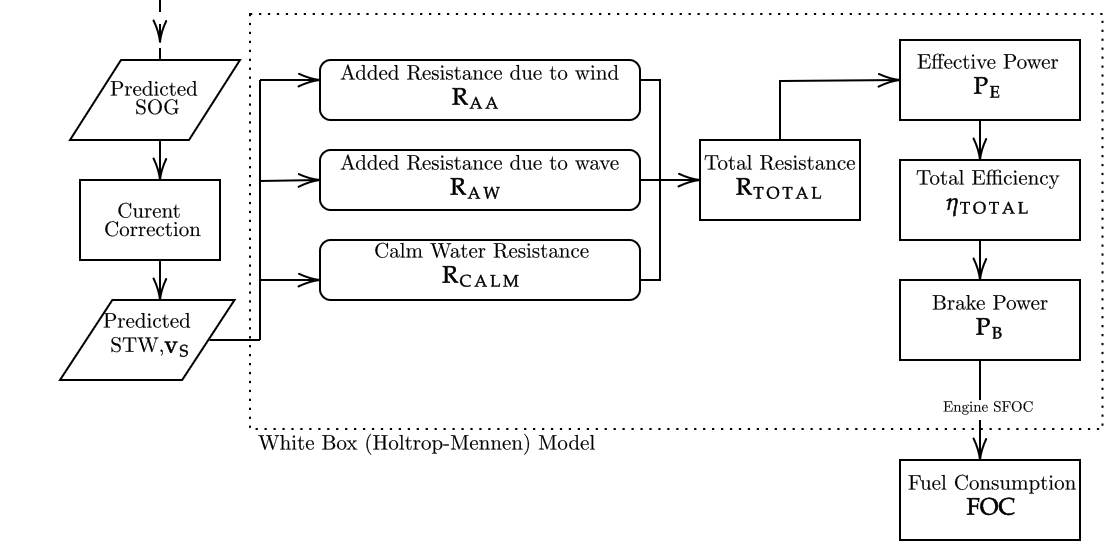
\includegraphics[width=\textwidth]{02_figures/flowmethod_WBM.png}
        \caption{Scheme of proposed WBM methodology adopted from \bcitet{XiaoLang.2020}}
        \label{fig:flowchart_WBM}
\end{figure}

The development process of GBM is summarised in \Cref{fig:flowchart_GBM}. Detailed discussion regarding the development of BBM and WBM model will be discussed in the following sections of this chapter.

\begin{figure}[h]
    \centering
        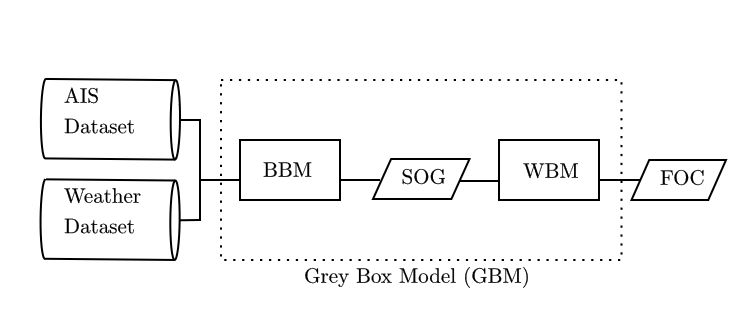
\includegraphics[width=.85\textwidth]{02_figures/flowmethod_GBM_alt.png}
        \caption{Scheme of proposed GBM methodology}
        \label{fig:flowchart_GBM}
\end{figure}


\section{Data Acquisition}\label{sec:data_acquisition}

The data is collected from a ferry serving between ports of K{\o}ge, R{\o}nne, Ystad and Sassnitz, as shown in \Cref{fig:Hammershus_journey_map} \bcitep{HammershusJourney}. The trip between K{\o}ge, R{\o}nne takes about 5 h 30 minutes and it sails between R{\o}nne and Sassnitz for 3 h and 20 minutes. The journey is tracked by T-AIS system of Danish Maritime Authority (DMA). The weather data along her sailing path are acquired from ECMWF\footnote{European Centre for Medium-Range Weather Forecast} with temporal resolution of 1 hour at granularity of 0.25° (longitude) x 0.25° (latitude), data from ECMWF provides information for wind, waves and seawater temperature. The information for current is obtained from CMEMS\footnote{Copernicus Marine Environment Monitoring Service} with temporal resolution of 3 hours at granularity of  0.25° (longitude) x 0.25° (latitude).\\ 

\begin{figure}[ht]
  \begin{minipage}{0.55\linewidth} % Adjust the width as needed
    \footnotesize
    \centering
    \begin{tabular}{l r}
        \hline
        IMO & 9812107 \\
        Type \& Service & Passenger ferry \\
        $L_{OA}$ & 158.00 m\\
        $L_{WL}$ & 144.80 m\\
        $B$ (moulded) & 24.5 m\\
        $T_{DESIGN}$ & 5.70 m\\
        $T_{MAX}$ & 5.85 m \\ 
        Gross Tonnage (GT) & 18,009 \\
        Deadweight (dwt) & 4,830 t \\
        Main Engines & Wärtsillä 8V31 2 x 4,880 kW \\
        SFOC & 169.4 g/kWh \\
        Service Speed & 17.7 knots \\
        Bow Thrusters & 2 x 1500 kW \\
        \hline
    \end{tabular}
    \caption{Particular of M/S Hammershus}
    \label{tbl:Hammershus_Data}
  \end{minipage}
  \hspace{0.01\linewidth}
%   \hfill
  \begin{minipage}{0.43\linewidth} % Adjust the width as needed
    \centering
    % \vspace*{0.1cm}
    \includegraphics[width=\linewidth]{02_figures/Bornholmerfærgen_route_map.png} % Replace example-image.jpg with your picture file name
    \caption{Journey of the ferry}
    \label{fig:Hammershus_journey_map}
  \end{minipage}
\end{figure}


\begin{figure}[h]
    \centering
        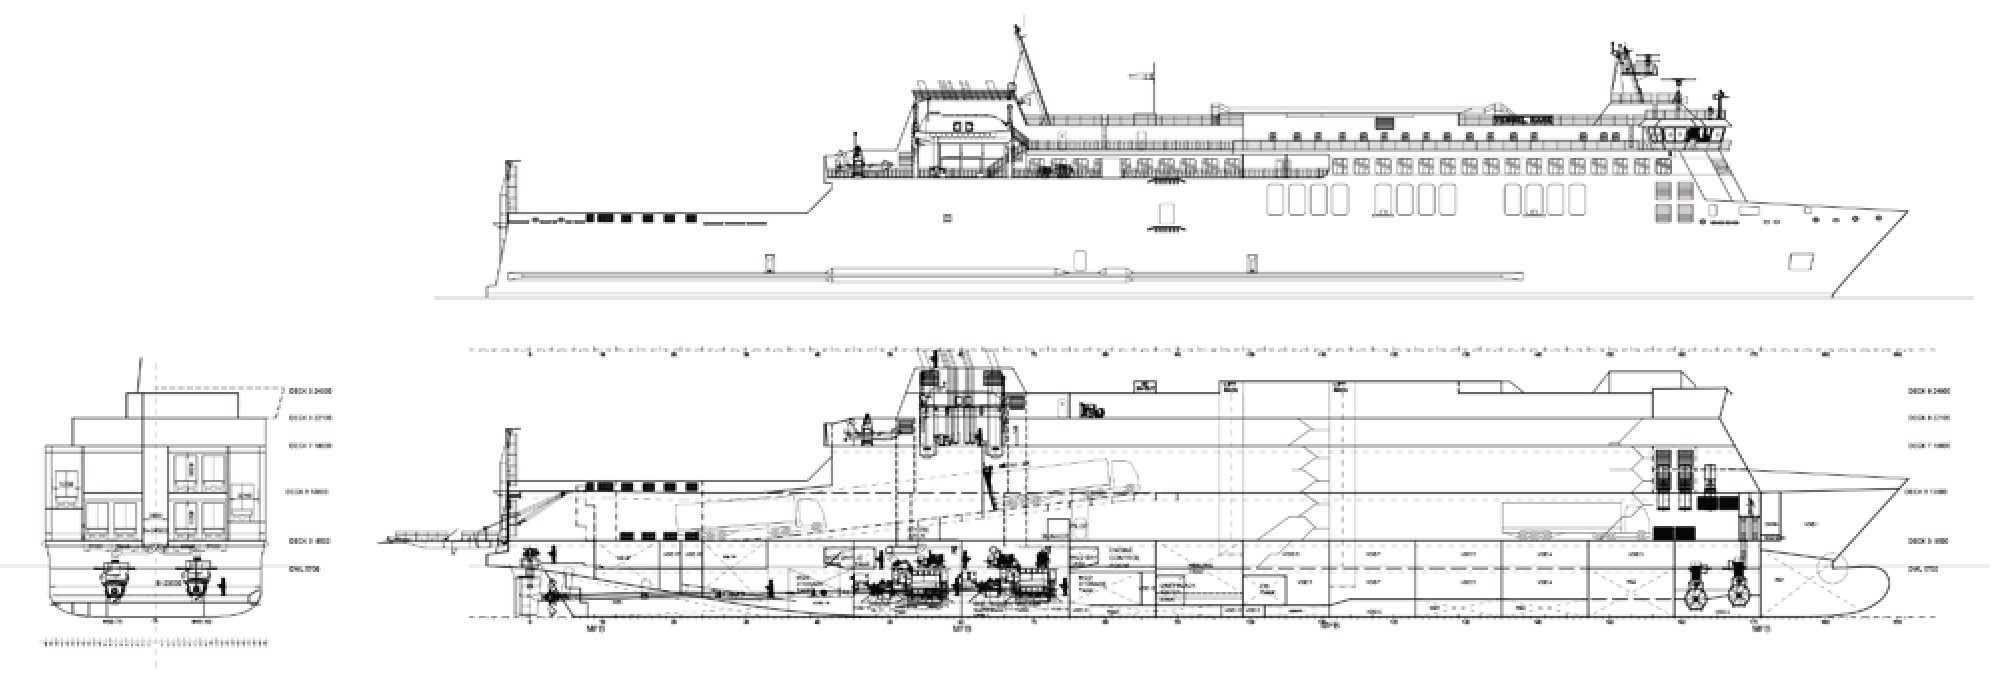
\includegraphics[width=\textwidth]{02_figures/Hammershus_Pict.jpg}
        \caption{Schematics of M/S Hammershus}
        \label{fig:Hammershus_Pict}
\end{figure}

The resulting fused dataset has a temporal resolution of 1 hour. Due to the difference in temporal resolution of the data from CMEMS and ECMWF, the weather information is synchronised so that the wind, waves, seawater temperature and sea current belongs to the same weather grid with same temporal resolutions. The features \textbf{wind direction},\textbf{swell direction}, and \textbf{wind wave direction} are oriented to true north. However, to reflect the actual direction of weather effects that are acting on the ship, these features are converted to true direction; where true direction is defined as the direction of weather effect with respect to the bow of the ship. The value ranges between 0° and 180°. Subsequently, through vector decomposition, the northward and eastward wind velocity is converted to absolute wind speed and wind direction \emph{with respect to True North},$\varphi$:

\begin{equation}\label{eqn:vwindabs}
    u_{\text{W}} = \sqrt{(u_{\text{W}_{N}})^2 + (u_{\text{W}_{E}})^2} 
\end{equation}
\begin{equation}\label{eqn:winddir}
    \varphi = 
    \begin{cases}
        360 - \arctan(u_{\text{W}_{E}} / u_{\text{W}_{N}}) \quad \text{\textbf{if}} \quad u_{\text{W}_{E}} > 0 \quad \wedge \quad u_{\text{W}_{N}} < 0 \\ 
        180 - \arctan(u_{\text{W}_{E}} / u_{\text{W}_{N}}) \quad \text{\textbf{if}} \quad u_{\text{W}_{E}} < 0 \quad \wedge \quad u_{\text{W}_{N}} > 0 \\ 
        270 - \arctan(u_{\text{W}_{E}} / u_{\text{W}_{N}}) \quad \text{\textbf{if}} \quad u_{\text{W}_{E}} > 0 \quad \wedge \quad u_{\text{W}_{N}} > 0 \\
        \arctan(u_{\text{W}_{E}} / u_{\text{W}_{N}}) \qquad \text{\textbf{otherwise}} 
    \end{cases}   
\end{equation}

Similarly, information of Northward and Eastward current Velocity is converted to absolute current speed and current direction \emph{with respect to True North} $\gamma$.\\ 

\begin{equation}\label{eqn:vcurrabs}
    v_{\text{C}} = \sqrt{(v_{\text{C}_N})^2 + (v_{\text{C}_E})^2} 
\end{equation}
\begin{equation}\label{eqn:currdir}
    \gamma = 
    \begin{cases}
        360 - \arctan(u_{\text{W}_{E}} / u_{\text{W}_{N}}) \quad \text{\textbf{if}} \quad v_{\text{C}_E} < 0 \quad \wedge \quad v_{\text{C}_N} > 0 \\ 
        180 - \arctan(u_{\text{W}_{E}} / u_{\text{W}_{N}}) \quad \text{\textbf{if}} \quad v_{\text{C}_E} > 0 \quad \wedge \quad v_{\text{C}_N} < 0 \\ 
        270 - \arctan(u_{\text{W}_{E}} / u_{\text{W}_{N}}) \quad \text{\textbf{if}} \quad v_{\text{C}_E} < 0 \quad \wedge \quad v_{\text{C}_N} < 0 \\
        \arctan(u_{\text{W}_{E}} / u_{\text{W}_{N}}) \qquad \text{\textbf{otherwise}} 
    \end{cases}   
\end{equation}

The initial dataset provides information to the true directions, which indicate the encounter direction of weather conditions with respect to the ship bow. Static information from the AIS data which only indicated the ship's identity and navigational status are discarded in the dataset. The initial structure have 27 features, 9 AIS features and 18 weather features. The structure of the initial dataset i.e. before data preprocessing and feature selection, is summarised in \Cref{tbl:dataset_init_struct} \\

\begin{table}[h!]
    \footnotesize
    \centering
    % \resizebox {\textwidth}{!}
    {\begin{tabular}{ p{0.4\textwidth} c }
    \hline
    \textbf{Feature} & \textbf{Feature Name}  \\
    \hline
    \multicolumn{2}{l}{\textbf{AIS data}}\\
    \hline
    Position Time Stamp [DD\slash MM\slash YYYY HH:MM:SS] & {\tt Time} \\
    Latitude [°] & {\tt LAT}   \\
    Longitude [°] & {\tt LON}  \\
    Width [m] & {\tt width}  \\
    Length [m] & {\tt length}\\
    SOG [Knots] & {\tt sog} \\
    COG [m/s] & {\tt cog}  \\
    Heading [°] & {\tt heading}  \\
    Draught [m] & {\tt draught} \\
    \hline
    \multicolumn{2}{l}{\textbf{Weather Data (0.5° Granularity)}}\\
    \hline
    Wind Speed [m/s] & {\tt windspeed} \\
    True North Wind Direction, $\varphi$ [°] & {\tt truenorthcurrentdir} \\
    Air Temperature Above Oceans [K] & {\tt oceantemperature} \\
    % Air Density Above Oceans [$\text{kg/m}^3$]& - \\
    Maximum Wave Height [m] & {\tt waveheight} \\
    % Swell Direction [°] & - \\
    % Wind Wave Direction & - \\
    Swell Period [s] & {\tt swellperiod} \\
    Wind Wave Period [s] & {\tt windwaveperiod}\\
    % Wave Direction [°] & - \\
    Wave Period [s] & {\tt waveperiod}\\
    Sea Surface Temperature [K] & {\tt surftemp}\\
    Combined Wind Wave Swell Height [m] &  {\tt windwaveswellheight} \\
    Swell Height [m] & {\tt swellheight}\\
    Wind Wave Height [m] & {\tt windwaveheight}  \\
    % Surface Pressure & - \\
    Current Speed [m/s] & {\tt curspeed} \\
    True North Current Direction $\gamma$ [°] & {\tt truenorthcurrentdir}\\
    True Wind Direction [°] & {\tt truewinddir}  \\
    True Current Direction [°] & {\tt truecurrentdir} \\
    True Swell Direction [°] & {\tt trueswelldir} \\
    True Wind Wave Direction [°] & {\tt truewindwavedir} \\
    True Wave Direction [°] & {\tt truewavedir} \\
    \end{tabular}}
\caption{Structure of fused dataset}\label{tbl:dataset_init_struct}
\end{table}

\section{Data Preprocessing}\label{sec:data_prep}

This section presents the steps taken during data preprocessing. The dataset will be subjected to data cleaning which include identification of anomalies and missing values. SOG threshold is applied to ensure that the model represent operating condition at steady state. Domain knowledge based, feature selection is performed to ensure the model does not violate vessel domain knowledge. The datasets then will be split to training, validation and test dataset. 

\subsection{Data Cleaning}\label{sec:data_cleaning}

The plot of the journey indicates that the journey between R{\o}nne and Sassnitz is not represented completely. This might be caused due to the limitation of T-AIS system which is caused by the due to poor coverage in the area between Sassnitz and R{\o}nne. This is shown by the plot shown in \Cref{fig:aiscoverage}. Therefore, the data plot for the journey between Sassnitz and R{\o}nne will be excluded. Basic threshold of decimal degrees of 55.04° N for latitude is applied, this threshold will exclude the journey between Sassnitz and R{\o}nne.\\

\begin{figure}
    \centering
        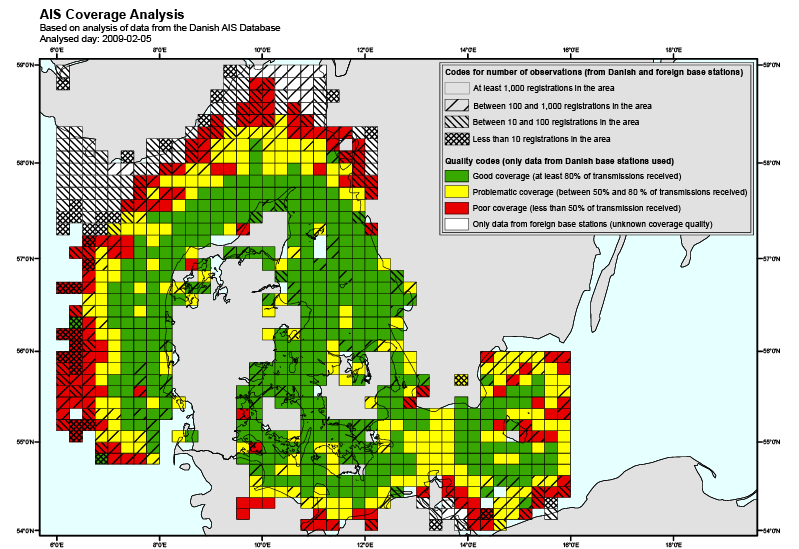
\includegraphics[width=0.8\textwidth]{02_figures/AIS_Coverage.png}
        \caption{Shore based AIS Coverage based on data from AIS database \cite{webaisdk.2023}}
        \label{fig:aiscoverage}
\end{figure}

In its initial state, the dataset contains 7453 data points which described the journey of the ship in one year. The initial data points represented all navigational status of the ship, which include ``mooring'', ``anchoring'' and ``underway using engine''. This is clearly observed in the histogram for the SOG \Cref{fig:anomalies_sog_curspeed}.\\ 

To ensure that the dataset represents the actual operating condition of ship in steady state, a threshold for SOG must be applied. SOG can vary due to changing sea state, but it can also be reduced by the ship's operator around the port when it departs from port of origin or arriving at port of arrival. Therefore, any data points with SOG less than 5 knots will be discarded which is considered as manoeuvring \bcitep{Abebe.2020,Yan.2020}. Post filtering, the amount of data points decrease significantly from 7453 data points to 3828 data points. This indicated that about half of the total data points represented the ship's stationary behaviour.\\

% \begin{figure}
%     \centering
%         \includegraphics[width=0.8\textwidth]{02_figures/SassnitznoFilter.png}
%         \caption{Journey of the ship in a year}
%         \label{fig:YearJourney}
% \end{figure}
\begin{figure}[h!]
    \centering
        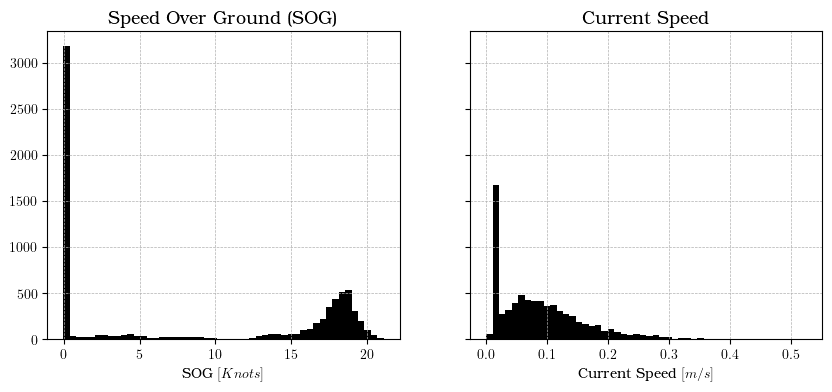
\includegraphics[width=0.9\textwidth]{02_figures/sog_curspeed_anomalies.png}
        \caption{Histogram plot of pre-filtered SOG and current speed}
        \label{fig:anomalies_sog_curspeed}
\end{figure}

From preliminary analysis, possible source of error is identified for data points representing current speed. In range of current speed between 0.01 and 0.03 $m/s$, noticeable peak in data points is observed as shown in \Cref{fig:anomalies_sog_curspeed}. This peak attributed to missing information on northward and eastward current speed in some data points from the provided dataset. This resulted in single random error value for current speed which resulted in the peak observed in the histogram.\\ 

\begin{figure}[h]
    \centering
        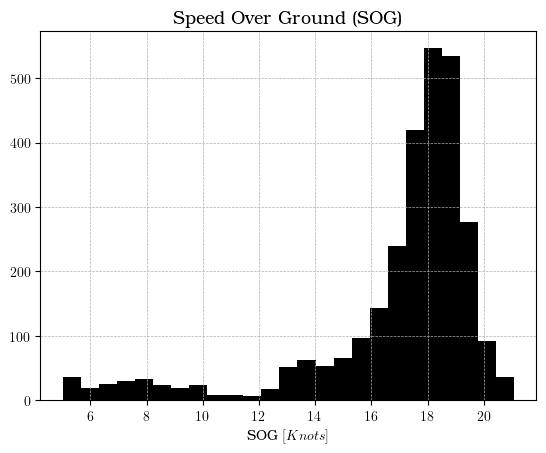
\includegraphics[width=0.6\textwidth]{02_figures/hist_init_sog_postfilter.png}
        \caption{Histogram plot of SOG after threshold}
        \label{fig:SOG_greater_five}
\end{figure}

To address the missing values, the missing values for eastward current and northward current are imputed using {\tt KNNImputer} feature from \scikit/. This is necessary as modelling package by \scikit/ cannot handle missing values. During imputing, each sample's missing values are imputed using the mean of nearest neighbour found in training dataset \bcitep{FabianPedregosa.2011}. Imputing strategy using k-nearest neighbour is considered as it should reflect the weather conditions within the region of missing values. Once the missing values of northward and southward current are imputed, the current speed for the missing values will be recalculated. The imputing approach using k-nearest neighbour is also applied to other weather features that contained missing values i.e. {\tt NaN} values.\\

\subsection{Feature Selection}\label{sec:feature_select}

To select appropriate features for the model, correlation between the features is first studied. Feature selection is necessary to simplify the model and subsequently save computing cost during training. Selection of features is based on statistical approach of High Correlation Filter proposed by Abebe et al. \bcitep{Abebe.2020}. This approach considers pairs of features with correlation features higher than 0.7 as one entity. However, the selection of highly correlated features must not violate physical knowledge. Therefore, the feature selection in this study is based on physical justification and this takes priority over purely statistical reasoning.\\

From AIS data, the information on \emph{time, latitude, longitude, width and length} are not included for training. Time, latitude and longitude only describe the location of the ship at a particular position and the width and length of ship are constant dimensions. As discussed in \Cref{sec:weather_definition}, the features \emph{combined wind wave swell height, swell height, maximum wave height and wind wave height} are physically correlated. The combined wind wave swell height defines the significant wave height $H_{1/3}$ and can be described using \Cref{eqn:H_sig_root}, \Cref{eqn:H_s_and_Tp} shows that the significant wave height also can be used to identify weather the sea is swell or wind sea dominated.\\

With that, it is clear that significant wave height should be retained for modelling, as many wave properties can be derived from it. The features swell height, wind wave height and maximum wave height will be dropped as it can be defined through significant wave height $H_{1/3}$. This decision is also statistically supported through the high correlation filter method. As shown in \Cref{fig:heatmap_ovr}, high correlation are obtained between the $H_{1/3}$, swell height, wind wave height and maximum wave height.\\

\begin{figure}[ht]
    \centering
    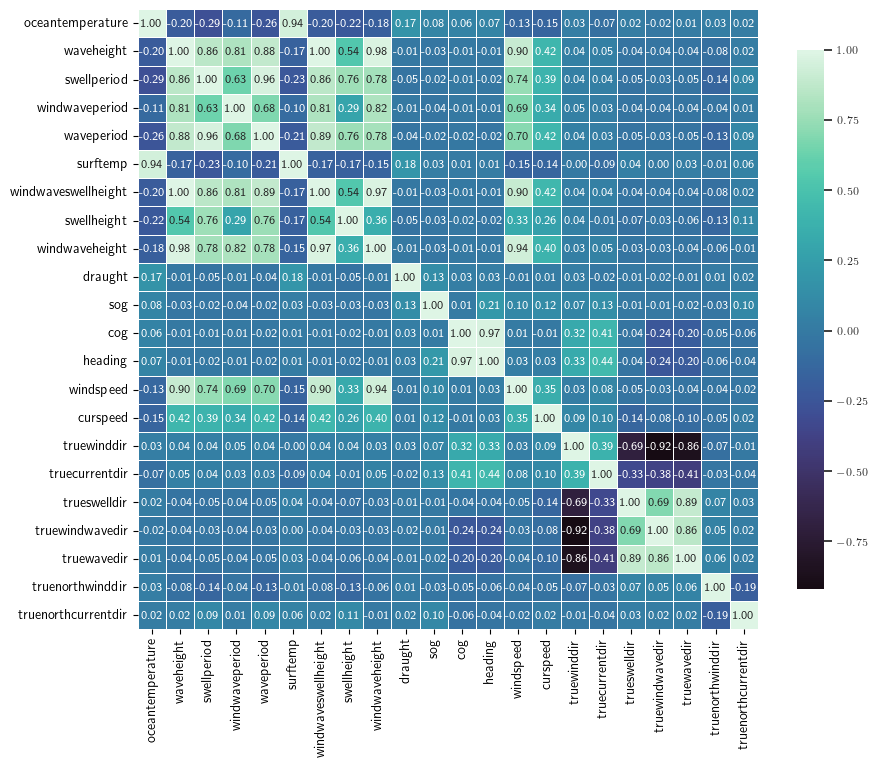
\includegraphics[width=.9\linewidth,height=.9\textheight,keepaspectratio]{02_figures/heatmap_corr_ovr.png}
    \caption{Correlation Heat Map}
    \label{fig:heatmap_ovr}
\end{figure}

From \Cref{fig:heatmap_ovr}, high correlation is observed between wave period, swell period and wind wave period. As discussed in \Cref{sec:weather_definition}, the sea state can be described through the significant height $H_{1/3}$ and spectral peak $T_p$ with help of Torsethaugen peak \bcitep{K.Torsethaugen.2004}. Hence, the features swell period and wind wave period are discarded as it only distinguish whether the sea is dominated by swell or by wind. The feature wave period will still be retained. As a result, the features ``true wind wave direction'' and ``true swell direction'' will be excluded from consideration since the features that account for their magnitude have been discarded.\\

Statistically, the heading and COG are highly correlated, but both features are retained as it explain two different parameters of the ship. Course Over Ground reflects the ship course heading while heading represented the actual heading of the ship at a particular point of time. Same principle also apply between air temperature above ocean and sea surface temperature. Air temperature above oceans represents the temperature of wind while sea surface temperature represents current temperature of current. From feature selection, 5 features from AIS data are discarded while 11 features are removed from the weather data. To predict the ship speed, The SOG will be selected as the label to train the model. The remaining attributes will be selected as training features. This is summarised in \Cref{tbl:struct_train_final}.\\

\begin{table}
    \footnotesize
    \centering
    % \resizebox {\textwidth}{!}
    {\begin{tabular}{ p{8cm}c }
    \hline
    \multicolumn{2}{l}{\textbf{Training Label}}\\
    \hline
    SOG [Knots] & {\tt sog} \\
    \hline
    \multicolumn{2}{l}{\textbf{Training Features}}\\
    \hline
    COG [°] & {\tt cog}  \\
    Heading [°] & {\tt heading}  \\
    Draught [m] & {\tt draught} \\
    Wind Speed [m/s] & {\tt windspeed} \\
    Air Temperature Above Oceans [K] & {\tt oceantemperature} \\
    % Maximum Wave Height [m] & {\tt waveheight} \\
    Wave Period [s] & {\tt waveperiod}\\
    Sea Surface Temperature [K] & {\tt surftemp}\\
    Combined Wind Wave Swell Height [m] &  {\tt windwaveswellheight} \\
    Current Speed [m/s] & {\tt curspeed} \\
    True Wind Direction [°] & {\tt truewinddir}  \\
    True Current Direction [°] & {\tt truecurrentdir} \\
    True Wave Direction [°] & {\tt truewavedir} \\
    \hline
    \end{tabular}}
\caption{Structure of training dataset}\label{tbl:struct_train_final}
\end{table}

\begin{table}
    \footnotesize
    \centering
    % \resizebox {\textwidth}{!}
    {\begin{tabular}{ p{0.23\linewidth} c c c c c c c c }
    \hline
    Features & Count & Mean & Std. & Min & 25\% & 50\% & 75\% & Max \\
    \hline
    \textbf{{\tt sog}} & 2871 & 16.91 & 3.18 & 5.03 & 16.56 & 17.94 & 18.72 & 21.07\\
    \hline
    {\tt cog} & 2871 & 196.47 & 85.93&	69.77 & 102.58& 188.01& 282.26& 355.07\\ 
    {\tt heading} & 2871 & 187.88&	88.47&	67.90&	100.86&	124.65&	279.19&	355.07\\
    {\tt draught} & 2871 &5.22& 0.18& 4.74& 5.11& 5.28& 5.38&5.67\\
    {\tt windspeed} & 2871 & 6.42 & 2.97 & 0.25 & 4.13 & 6.15 &	8.36 & 16.01\\
    {\tt oceantemperature}\tablefootnote{Air temperature above oceans}& 2871 & 282.71 & 6.49 & 264.08& 277.13& 282.64& 288.82& 296.83 \\
    {\tt waveperiod} & 2871& 3.66& 0.82& 1.86& 3.07& 3.57& 4.14& 7.05\\
    {\tt surftemp}\tablefootnote{Sea Surface Temperature}&2871 &283.40& 5.73& 273.05& 278.13& 282.83& 288.86 &294.75\\
    {\tt windwaveswellheight}\tablefootnote{Significant wave height}  &  2871 & 0.75 & 0.51 & 0.07 &0.38 &	0.64 &	0.95 &  3.70  \\
    {\tt curspeed} & 2871 &0.10& 0.07& 0.00 & 0.05& 0.08 & 0.13 & 0.53\\
    {\tt truewinddir} & 2871 & 87.14 & 55.96 &	0.00 & 34.19 &	84.79 & 140.58 & 179.77	\\
    {\tt truecurrentdir} & 2871 & 89.15 & 57.53 & 0.25 & 31.01 & 86.78 & 143.32 & 179.99 \\
    {\tt truewavedir} & 2871 & 91.74 & 55.53& 0.13& 39.12 & 92.28 & 143.33 & 179.92 \\
    \hline
    \end{tabular}}
\caption{Descriptive statistics of preprocessed dataset}\label{tbl:dataset_descriptive_pretraining}
\end{table}

\begin{figure}
    \centering
    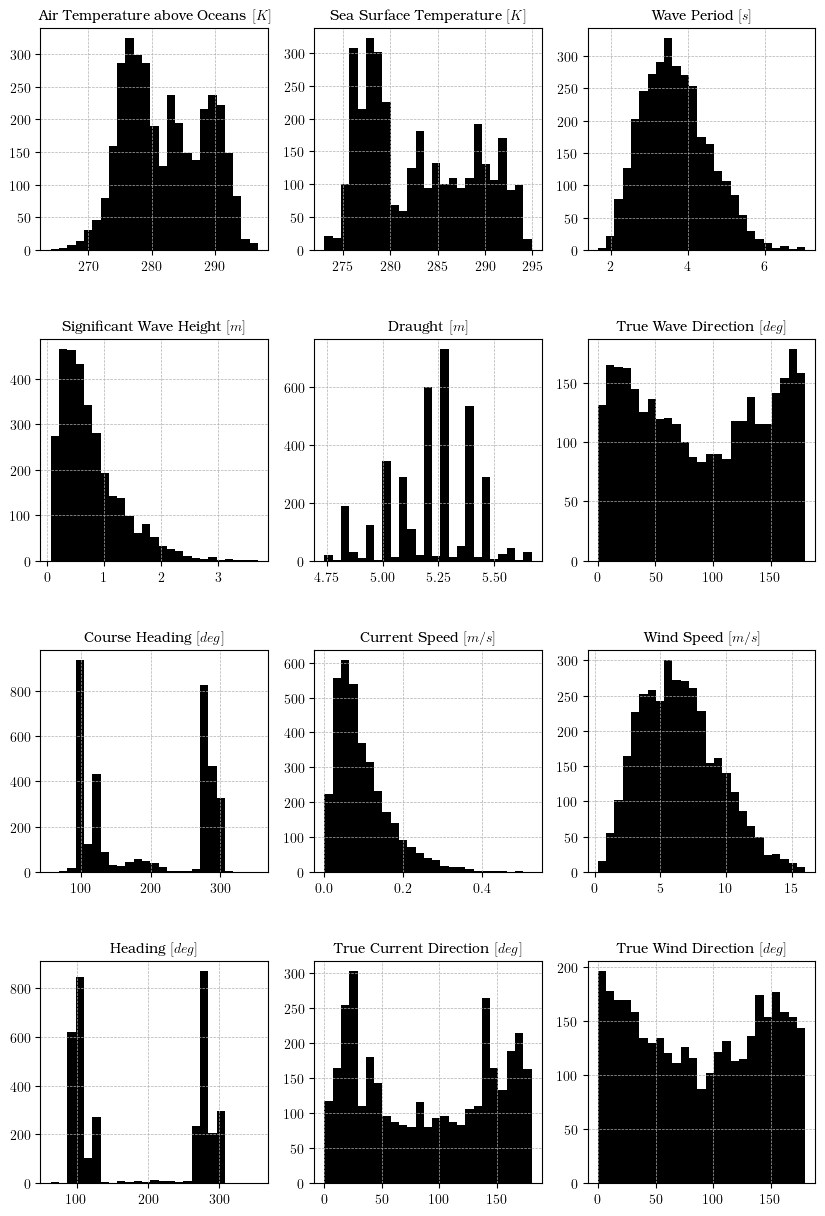
\includegraphics[width=.9\linewidth]{02_figures/hist_init_preprocessing.png}
    \caption{Histogram of training features}
    \label{fig:hist_training_ftr_label}
\end{figure}

\pagebreak

\section{Black Box Modelling}\label{sec:BBM_modelling}

In this section, the modelling of ship speed through SOG using selected features will be performed using tree-based regressor model. The tree-based regressor model considered are decision tree regressor (DTR), random forest regressor (RFR) and extra-tree regressor (ETR). The tree-based models are compared against multiple linear regressor (MLR) for benchmarking. For training, the dataset is split into training and test dataset in ratio of 75:25. This corresponds to 2871 data points for training and 957 data points for testing. The training dataset will be subjected to 10-fold splitting, this k-fold splitting is performed as the model will be evaluated using k-fold cross validation. The hyperparameter of the tree-based regressor will be iteratively tuned until no further improvements of the model can be made.\\


\subsection{Performance Metrics for Validation}\label{sec:perf_metrics}

To gain sensible estimate of model performance and how precise a model is, the model will be cross validated by means of k-folding. K-fold cross validation split the training set into k subsets which is called \emph{folds}, then the model will be trained k times using k-1 subsets and remaining one for validation, this process is illustrated in \Cref{fig:kfold}. For each iteration, each model is evaluated using different performance metrics such as \textbf{Coefficient of Determination ($R^2$), Explained Variance (EV), Mean Absolute Error (MAE),Root Mean Square (RMSE), Median Absolute Deviation (MAD) and Mean Absolute Percentage Error (MAPE)}. The results from each iteration is then averaged, where the information on model precision can be gained from the standard deviation. Performing k-fold cross validation checks model robustness against different datasets. The properties of each performance metric will be discussed in the following sections.

\begin{figure}
    \centering
    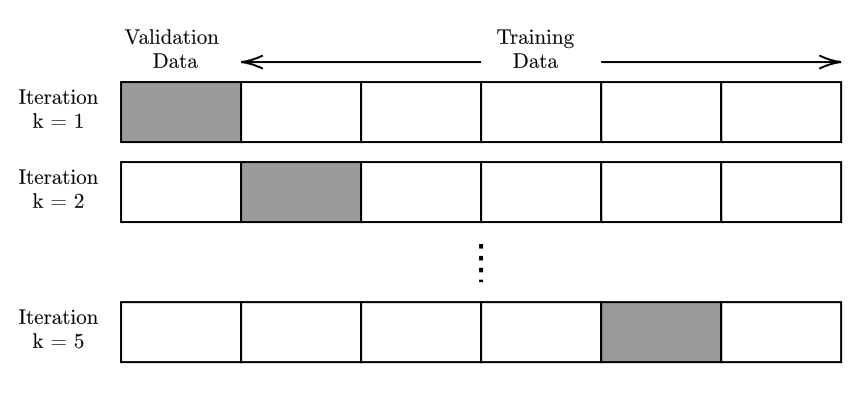
\includegraphics[width=.85\textwidth]{02_figures/kfold.png}
    \caption{Visual illustration of k-folding, Grey shaded box represents the validation data while white box represents the training data}
    \label{fig:kfold}
\end{figure}

\subsubsection*{Coefficient of Determination ({$R^2$})}\label{sec:rsquared}

The coefficient of determination $R^2$ gives a measure on prediction quality, $R^2$ quantifies the ability of the regression model to approximate the actual values. $R^2 $ is defined by \Cref{eqn:rsquared}, where $y$ represents true target output, $\hat{y}$ represents the predictor output and $\overline{y}$ represents the mean. $R^2$ score range between 0 and 1, higher values i.e. $R^2 \rightarrow 1$ indicate better model fit and score of 1 indicate perfect prediction.\\

\begin{equation}\label{eqn:rsquared}
    R^2(y,\hat{y}) = 1 - \frac{\sum_{i = 1}^{n} (y_{\text{i}} - \hat{y}_{\text{i}} )^2 }{\sum_{i = 1}^{n} (y_{\text{i}} - \overline{y}_{\text{i}})^2} \quad \textbf{where} \quad \overline{y} = \frac{1}{n}\sum_{1}^{n} y_\text{i}
\end{equation}

\subsubsection*{Explained Variance (EV)}\label{sec:expVar}

Explained variance indicate how well a model can capture variance from a dataset. It is defined by \Cref{eqn:expVar}, where $\sigma_x$ represents standard deviation of parameter $x$. EV score range between 0 and 1, where the best score of $EV = 1$ can be obtained if $\sigma^2_{(y-\hat{y})} \rightarrow 0$.\\  

\begin{equation}\label{eqn:expVar}
    EV(y,\hat{y}) = 1 - \frac{\sigma^2_{(y-\hat{y})}}{\sigma^2_{y}}
\end{equation}

\subsubsection*{Mean Absolute Error (MAE)}\label{sec:MAE}

MAE indicated the expected value of absolute ($L^1$ norm) error, and it can be calculated by:

\begin{equation}\label{eqn:MAE}
    MAE(y,\hat{y}) = \frac{1}{n}\sum_{i=1}^{n} |y_{\text{i}} - \hat{y}_{\text{i}}| 
\end{equation}

\subsubsection*{Root Mean Square Error (RMSE)}\label{sec:RMSE}

The RMSE describe the expected value of quadratic error. RMSE place large penalty on large deviation between true and estimated values and for this reason, it can be used to as a metric to indicate model performance against outliers. Ideal score is observed when $\text{RMSE} \rightarrow 0$. RMSE can be considered as absolute measure of model fitness. Omitting the root term, RMSE becomes MSE, which is the loss function of \Cref{eqn:costfun} that is used to determine the most optimal split in a regression decision tree.\\

\begin{equation}\label{eqn:RMSE}
    RMSE(y,\hat{y}) = \sqrt{\frac{1}{n}\sum_{i=1}^{n} (y_{\text{i}} - \hat{y}_{\text{i}})^2} 
\end{equation}

\subsubsection*{Median Absolute Deviation (MAD)}\label{sec:MAD} 

MAD is a performance metrics that considers the median of the absolute errors. It is robust to outlier as it only consider median performance

\begin{equation}\label{eqn:MAD}
    MAD(y,\hat{y}) =  \text{median} (|y_{\text{1}} - \hat{y}_{\text{1}}|,\dots,|y_{\text{i}} - \hat{y}_{\text{i}}|)
\end{equation}

\subsubsection*{Mean Absolute Percentage Error (MAPE)}

Is an alternative to MAE, which provide easier interpretation, the result of MAPE can be interpreted according to \Cref{eqn:MAPE} \bcitep{MontanoMoreno.2013}. The usage of MAPE in model evaluation is to get initial estimate, as MAPE comes with some drawback such as instability when $y_i = 0$ and it may lead to biased forecast \bcitep{Gkerekos.2019}. As such, the evaluation of the model performance will be mainly based on MAE and RMSE.    

\begin{equation}\label{eqn:MAPE}
    MAPE(y,\hat{y}) = \frac{1}{n}\sum_{i=1}^{n} \biggl|\frac{y_{\text{i}} - \hat{y}_{\text{i}}}{y_i}\biggr| \cdot 100\%  \quad \textbf{with} \quad \begin{array}{l c}
        \text{MAPE} & \text{Interpretation}\\
        \hline
        < 10 & \text{Highly accurate forecasting} \\
        10-20 & \text{Good Forecasting} \\
        20-50 & \text{Reasonable forecasting}\\
        > 50 & \text{Inaccurate forecasting} \\
        \hline
    \end{array}
\end{equation}

\pagebreak

\subsection{Model Hyperparameter Optimisation}\label{sec:hpo}

The subject of parameter tuning was briefly discussed in \Cref{sec:dt_theo}. In \Cref{sec:dt_theo} parameter tuning was applied to decision tree regressor to avoid overfitting by changing the minimum amount of samples a leaf node has. This example implies that altering model hyperparameter will affect the model performance. However, the optimisation of the hyperparameter cannot be performed \emph{a priori} and as such iterative process will be performed until best hyperparameter value is found.\\ 

% \begin{table}[ht]
%     \scriptsize
%     \centering
%     % \resizebox {\textwidth}{!}
%     {\begin{tabular}{ p{0.33\textwidth}p{3cm}p{3cm}p{3cm}  }
%     \hline
%     \multicolumn{1}{c}{\textbf{Model}} & \multicolumn{1}{c}{\textbf{Decision Tree}}  & \multicolumn{1}{c} {\textbf{Random Forest}} & \multicolumn{1}{c}{\textbf{Extra-Trees}}\\
%     \hline
%     Number of trees & \multicolumn{1}{c}{1} & \multicolumn{1}{c}{Many} & \multicolumn{1}{c}{Many}\\
%     Features considered for split at each node &   \multicolumn{1}{c}{All features}  & \multicolumn{1}{c}{Random subset of features} & \multicolumn{1}{c}{Random subset of features} \\
%     Bootstrapping & \multicolumn{1}{c}{Not applied} & \multicolumn{1}{c}{Yes} & \multicolumn{1}{c}{No}\\
%     Split Rule  & \multicolumn{1}{c}{Best split} & \multicolumn{1}{c}{Best split}& \multicolumn{1}{c}{Random split}\\
%     \end{tabular}}
% \caption{Comparison of tree based model from \Cref{sec:tree_intro}}\label{tbl:table_trees}
% \end{table}

\scikit/ offers {\tt GridSearchCV} and {\tt RandomizedSearchCV} to help search for the most optimal hyperparameter. Both solutions operate with similar principle: The selected hyperparameters to be tuned with its value range is evaluated using cross validation to evaluate the best possible combination between the selected hyperparameters. The difference between {\tt GridSearchCV} and {\tt RandomizedSearchCV} lies in how it searches for the best value for the selected hyperparameters: {\tt GridSearchCV} involves construction of grids containing all possible combinations of hyperparameter value in specified range.{\tt RandomizedSearchCV} randomly samples hyperparameter values.\\ 

The exhaustive nature of {\tt GridSearchCV} means that it is computationally costly to perform, especially when there are multiple hyperparameters to be considered and value search space is large. {\tt RandomizedSearchCV} gives more control to computing budget by setting the number of iteration and usually produces more accurate results than {\tt GridSearchCV} approach. \bcitep{Geron.2019,J.Bergstra.2012}. \\

For this reason, the {\tt RandomizedSearchCV} will be employed to search for best possible hyperparameter. However, the limitation of \emph{a priori} knowledge of hyperparameter value still exists. In spite of {\tt RandomizedSearchCV} ability to control the computational budget, it is still takes considerable time to obtain the best hyperparameter value. The computational budget may be spent on searches in unpromising search space. With that, initial exploration on the effect of each hyperparameter on model performance will be performed to give better overview on which search space that should be considered during hyperparameter optimisation. In the next subsections, the effect of tunable hyperparameter of tree-based model from \scikit/ will be explored to give baseline numbers for the search space. RMSE is used as performance metrics as the hyperparameter parameter optimisation done in this thesis aims to reduce the error during prediction. \\ 

\subsubsection*{Number of features}\label{sec:max_features}

Defined with default value as {\tt max\_features=None} in \scikit/. This hyperparameter controls the number of features to be considered when looking for the best split, the default {\tt None} option means it will consider all features. This parameter tuning is available for Decision Tree Regressor, Random Forest Regressor and Extra-Tree Regressor. Initial exploration indicated Random Forest Regressor and Extra Tree Regressor benefit from considering more features. Decision Tree Regressor also benefits from considering all features for determining the split.\\ 

\begin{figure}[h]
    \centering
        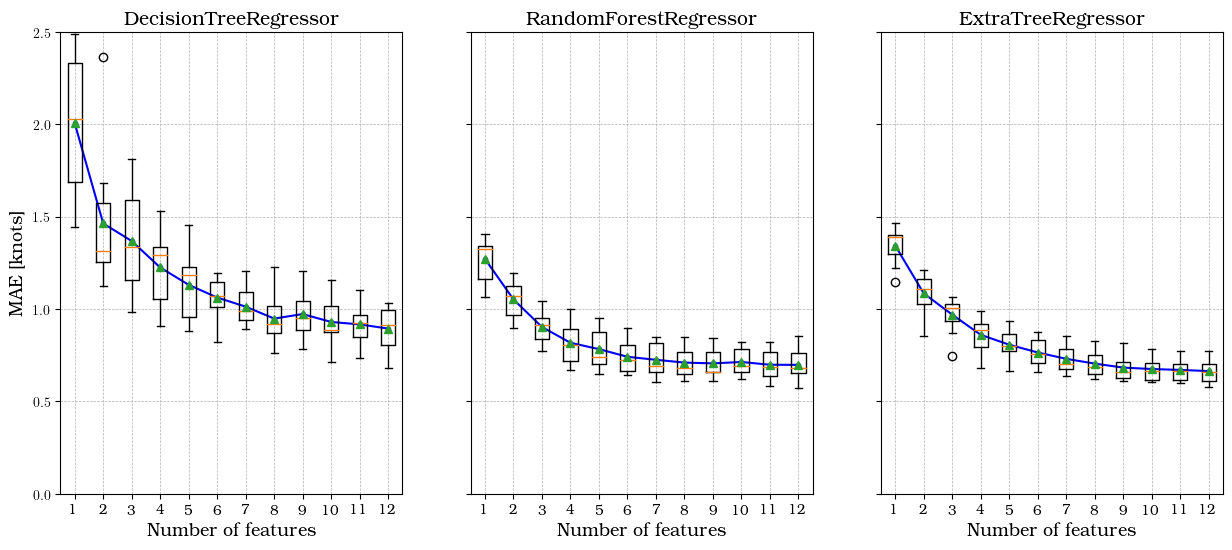
\includegraphics[width=.9\textwidth]{02_figures/hpo_n_features_mae.png}
        \caption{Hyperparameter tuning of {\tt max\_features}}
        \label{fig:hpo_n_features}
\end{figure}

\subsubsection*{Minimum samples to split a node}\label{sec:min_samples_split}

Defined with default value as {\tt min\_samples\_split=2} in \scikit/. This hyperparameter controls the minimum number of samples i.e. data points required to split a node. The default value of {\tt 2} is the least number of sample required to split a node i.e. 1 sample is split to the left and right branch respectively. The plot at \Cref{fig:hpo_min_samples_leaf} indicates that tuning this hyperparameter will not have any major impact on any model's performance.\\
\begin{figure}[h]
    \centering
        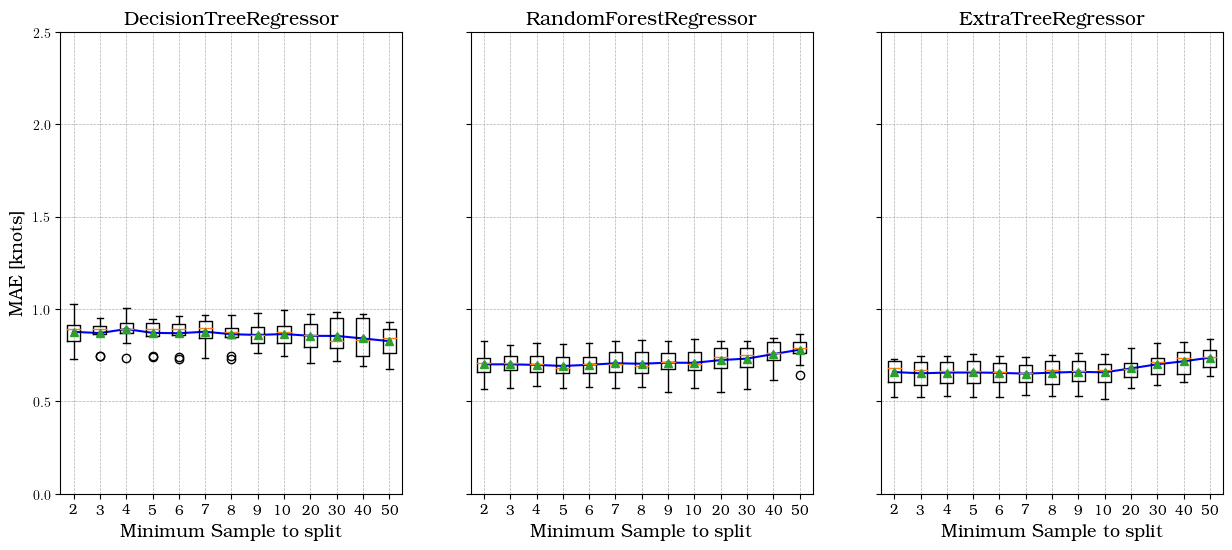
\includegraphics[width=.9\textwidth]{02_figures/hpo_min_samples_split_mae.png}
        \caption{Hyperparameter tuning of {\tt min\_samples\_split}}
        \label{fig:hpo_min_samples_split}
\end{figure}

\pagebreak

\subsubsection*{Number of sample in a leaf node}\label{sec:min_samples_leaf}

Defined with default value as {\tt min\_samples\_leaf=1} in \scikit/. This parameter controls number of samples required to be at leaf node, where split point will be considered if the leaf contains at least {\tt min\_samples\_leaf=n} training samples in each left and right branch. As shown in \Cref{fig:geron6_6}, tuning this hyperparameter to higher values helps to smoothen the model and avoid overfitting. However, this may lead to underfitting as the model is unable to capture the trend within the data. This is supported by the findings shown in \Cref{fig:hpo_min_samples_leaf}, the DTR benefits from regularisation at certain breakeven point. But, after this breakeven point, the model's performance degrades. It is also observed that tuning this parameter will have a negative impact on RFR and ETR model's performance-  

\begin{figure}[h]
    \centering
        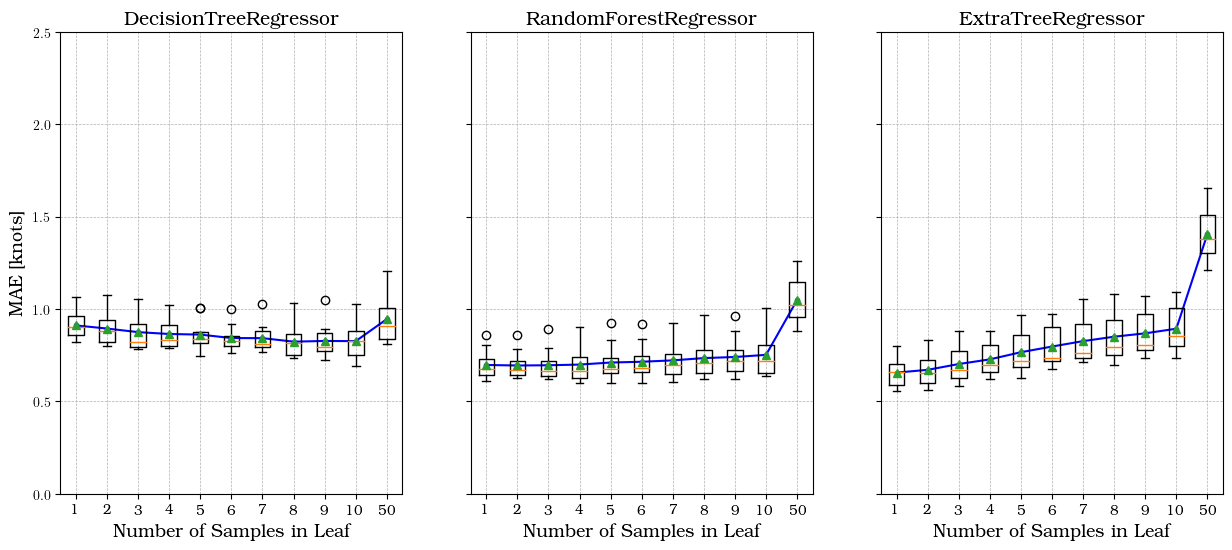
\includegraphics[width=.9\textwidth]{02_figures/hpo_min_samples_leaf_mae.png}
        \caption{Hyperparameter tuning of {\tt min\_samples\_leaf}}
        \label{fig:hpo_min_samples_leaf}
\end{figure}

\subsubsection*{Depth of Tree}\label{sec:max_depth}

Defined with default value as {\tt max\_depth=None} in \scikit/. This hyperparameter controls the growth of the tree. Leaving it at {\tt max\_depth=None} means the tree will grow until all leaves are pure i.e. until minimum MSE is obtained or when the number of samples is less than the minimum number of samples required to split an internal node. Similar to {\tt min\_samples\_leaf}, DTR shows improvement until a certain breakeven point. RFR performance seems to stabilise at certain depth while ETR benefits from allowing full growth of the tree. It can also be observed that the model's performance are identical for {\tt max\_depth=1}, which is evident as shown in \Cref{fig:hpo_max_depth}  

\begin{figure}[h]
    \centering
        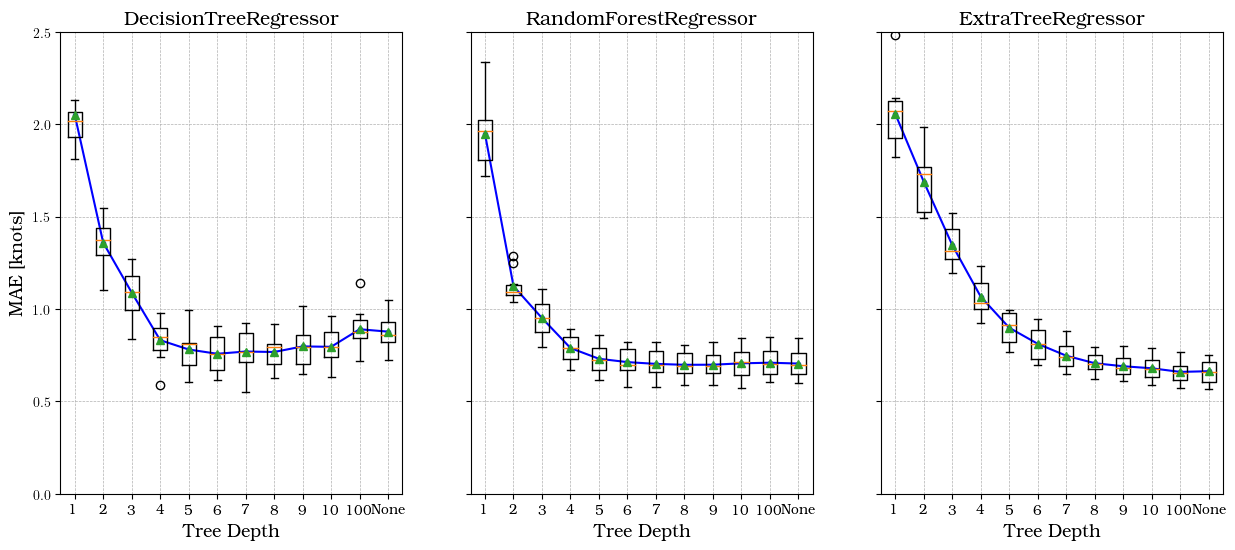
\includegraphics[width=.9\textwidth]{02_figures/hpo_max_depth_mae.png}
        \caption{Hyperparameter tuning of {\tt max\_depth}}
        \label{fig:hpo_max_depth}
\end{figure}

\subsubsection*{Number of Trees}\label{sec:n_estimators}

Defined with default value as {\tt n\_estimators=100}. This hyperparameter controls the amount of trees i.e. predictors in a forest. Tuning of number of trees will have an effect on the training time, and it is only available to RFR and ETR. The default value seems to yield satisfactory result, as the performance for both RFR and ETR stabilise after in this case stabilise after 100 trees, as seen in \Cref{fig:hpo_n_features}.
\begin{figure}[h]
    \centering
        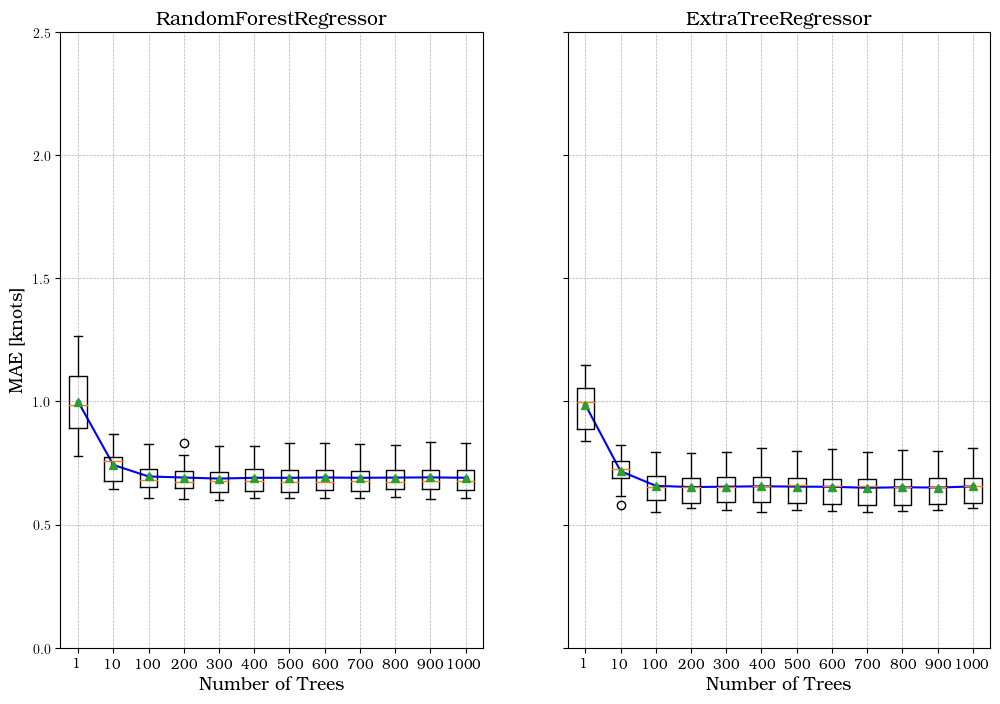
\includegraphics[width=.65\textwidth]{02_figures/hpo_n_estimators_mae.png}
        \caption{Hyperparameter tuning of {\tt n\_estimators}}
        \label{fig:n_estimators}
\end{figure}

 

\clearpage

\section{White Box Modelling}\label{sec:WBM_modelling}

In this section, the predicted SOG from the BBM will be fed into the WBM to predict the fuel consumption (FOC). Using Holtrop-Mennen approximation method, the resistance encountered by the ship will be estimated to find the total resistance which will be used to calculate the power required to propel the ship. However, during resistance calculation, some form coefficients and ship parameters are not readily available and may need to be assumed based on other literature studies, this assumption will be indicated throughout this section. The resulting brake power $P_B$ is plotted against the STW $v_S$ to obtain a power speed curve model which can be used to predict FOC. 

\subsection{Calculation of Total Resistance}\label{sec:Rtot_calc_method}

The formula used to calculate total resistance $R_{TOTAL}$ in this section are presented in \Cref{sec:holtrop_mennen_calc} with principle dimension of the ship which was given in \Cref{tbl:Hammershus_Data}. Some assumptions are made for the sea state and the values of some form coefficients are calculated based on empirical formulas presented in \Cref{sec:Ship_design_param}. In this case study, Holtrop-Mennen method can be used as it fulfills the condition set in \Cref{eqn:holtrop_cond}:
\begin{equation}
    \label{eqn:holtrop_cond_fulfill}
    % \begin{multlined}
    \begin{gathered}
        Fr = 0.2417  \leqslant 0.45 \\
        0.55 \leqslant C_P = 0.6707 \leqslant 0.85 \\
        3.9 \leqslant \frac{L}{B} = 5.91 \leqslant 9.5
    \end{gathered}
    % \end{multlined}
\end{equation}

The calculations of resistance are dynamics as the Froude number $Fr$ is based on $v_S$, the design Froude number $Fr_{DESIGN}$ is used to check use cases for some equations.

\subsubsection*{Calculation of frictional resistance $R_F$}

For the calculation of surface area of bare hull $S$, it is assumed that the aft has a U-shaped section. Then the appropriate $C_{stern}$ can be calculated to obtain the constant $c_{14}$ \Cref{eqn:c_14}. For the calculation of length of run $L_R$, approximation for $\ell_{CB}$ are made based on \Cref{eqn:lcb}. The constants $c_{14}$ and $L_R$ are used to calculate the form factor $1+k_1$ which will be used to calculate $R_F$.

\subsubsection*{Calculation of appendage resistance $R_{APP}$}

From known ship information and ship schematics shown in \Cref{fig:Hammershus_Pict}, it can be deducted that the ship consists of the following appendages:

\begin{itemize}
    \setlength\itemsep{0em}
    \item Two high-lift flap rudders
    \item Single centre skeg
    \item Twin shafts supported by two brackets
\end{itemize}

The assumptions for the appendage area are made by scaling the schematics to known measurements (e.g. the $L_{WL}$). From here, the appropriate $k_{2_i}$ constants for individual appendages will be selected to obtain the $(1+k_{2_i})_{eq}$ from \Cref{eqn:k2eq}.

\begin{table}[h]
    \footnotesize
    \centering
    % \resizebox {\textwidth}{!}
    {\begin{tabular}{ p{0.2\linewidth} c c}
    \hline
    Appendage type & Value & $(1+k_{2_i})$ \\
    \hline
    \multicolumn{2}{l}{\textbf{Two high-lift flap rudders}} & 3\\
    \hline
    $h_{\text{RUDDER}}$ & 4.06 $m$\\
    $B_{\text{RUDDER}}$ & 1.99 $m$\\
    $S_{\text{RUDDER}}$ & 16.16 $m^2$\\
    \hline
    \multicolumn{2}{l}{\textbf{Single centre skeg}} & 1.5\\
    \hline
    $h_{\text{SKEG}}$ & 4.41 $m$\\
    $B_{\text{SKEG}}$ & 26.23 $m$\\
    $S_{\text{SKEG}}$ & 115.67 $m^2$\\
    \hline
    \multicolumn{2}{l}{\textbf{Twin shafts supported by two brackets}} & 3\\
    \hline
    $D_{\text{SHAFT}}$ & 0.55 $m$\\
    $L_{\text{SHAFT}}$ & 13.54 $m$\\
    $S_{\text{SHAFT}}$ & 46.79 $m^2$\\
    \hline
    \multicolumn{1}{l}{\textbf{$S_{APP_{tot}}$}} & \textbf{178.62} $m^2$ \\
    \multicolumn{2}{l}{\textbf{$(1+k_{2_i})_{eq}$}} & \textbf{2.03} \\
    \end{tabular}}
\caption{Assumed appendage values}\label{tbl:assume_appendage_dimension}
\end{table}

Additionally, there are two bow thrusters installed with approximated diameter of $d_{TH}= 2.15 m$, from here, the constant $C_{D_TH}$ can be approximated using \Cref{eqn:R_th}. Hence, the appendage resistance $R_{APP}$ can be calculated using \Cref{eqn:R_app}.

\subsubsection*{Calculation of wave resistance $R_{W}$}

The calculation of wave resistance is based on the case for $Fr \leq 0.4$ using equation \Cref{eqn:R_w_low}. The estimation is done by adding the constants presented between \Cref{eqn:c_7} and \Cref{eqn:m4}. There are some use cases for some equations, which is summarised in \Cref{tbl:R_w_use_case}.

\begin{table}[h]
    \footnotesize
    \centering
    % \resizebox {\textwidth}{!}
    {\begin{tabular}{ p{0.2\linewidth} c c }
    \hline
    Constant & Use Case & Equation \\
    \hline
    $c_7$ &  $0.11 < \frac{B}{L_{WL}} \leq 0.25$ & \Cref{eqn:c_7} \\
    $c_{15}$ & $\frac{L_{WL}^2}{V} \leq 512$ & \Cref{eqn:c15} \\
    $c_{16}$ & $C_P \leq 0.8$ & \Cref{eqn:c16} \\
    $\lambda$ & $L_{WL} \leq 12$ & \Cref{eqn:lambda} \\
    \hline
    \end{tabular}}
\caption{Use case of constants for $R_W$}\label{tbl:R_w_use_case}
\end{table}

\subsubsection*{Calculation of bulbous bow resistance $R_B$}
The area $A_{BT}$ used to calculate is approximated based on \bcitet{Kracht.78} with:

\begin{equation}
    \label{eqn:A_BT}
    A_{BT} = 0.085 A_M
\end{equation}

For the height $h_B$, the upper limit of $h_B = 0.6T_{DESIGN}$ is selected, and it is assumed that $T_F = T_{DESIGN}$.

\subsubsection*{Calculation of (immersed) transom resistance $R_{TR}$}

Since the immersed transom area is unknown, \bcitet{Rakke2016} approximated the immersed transom area based on correlation of ship dimension from literature review of \bcitet{Holtrop.1982}:

\begin{equation}
    \label{eqn:A_TR}
    A_{TR} = 0.051 A_M
\end{equation}

This approximation must be used with caution as it is only based on case study of \bcitet{Holtrop.1982}. However, to author's best knowledge, there are no other literature that provide empirical estimation of $A_{TR}$. Therefore, this estimation will be selected in this case study. The selection for the value of constant $c_6$ is dependent on the value of $Fr_T$, which is a function of $v_S$. From there, the transom resistance can be calculated using \Cref{eqn:R_transom}

\subsubsection*{Calculation of correlation allowance resistance $R_A$}

The selection of constant $c_4$ in equation \Cref{eqn:c4} is based on the $T_F$, then the correlation resistance $R_A$ can be calculated using \Cref{eqn:R_a}.

\subsubsection*{Calculation of added resistance due to wind $R_{AA}$}

Two assumptions are made during the calculation of $R_{AA}$, since the information of lateral area $A_L$ and $A_F$ are not readily available, these values are assumed based on the dimension of similar ferry in the case study of \bcitet{Blendermann.1994}. It is assumed that the ferry has an $A_L$ of \textbf{2125.80} $m^2$ and $A_F$ of \textbf{325.30} $m^2$. From \Cref{tbl:BlendermannCoeff}, the case for ferry ship is taken to get the necessary constants for the calculation of $R_{AA}$. 

\subsubsection*{Calculation of added resistance due to wave $R_{AW}$ }

This part of the equation is relatively straightforward, $L_{BWL}$ will be approximated to about \textbf{43.75} m. The calculation of $R_{AWL}$ will be based on the data of significant wave height $H_{1/3}$ from the dataset.

\pagebreak

\subsection{Calculation of total efficiency $\eta_{TOT}$}\label{sec:eta_tot_method}

\subsubsection*{Calculation of open water efficiency $\eta_O$}

This value is approximated based on the line of Wageningen series in \Cref{fig:breslin_open water efficiencies} \bcitep{Breslin.1994}. The case will be for ``Passenger ships and high speed naval vessels''. Since the value of $C_{Th}$ is not available, the value of $\eta_O$ is approximated as \textbf{0.7}.

\subsubsection*{Calculation of hull efficiency $\eta_H$}

For the calculation of $\eta_H$, the value of the propeller diameter $D$ is approximated as \textbf{4 m}, which is based on the schematics of the ship shown in \Cref{fig:Hammershus_Pict}.

\subsubsection*{Calculation of relative rotative efficiency $\eta_R$}

The missing value required to compute \Cref{eqn: eta_rot_holtrop} is the pitch-diameter propeller ratio. This value will be estimated as $P/D =$ \textbf{1.135}, which is obtained from the work of \bcitet{Bertram.2000}.

\begin{figure}[h]
    \centering
        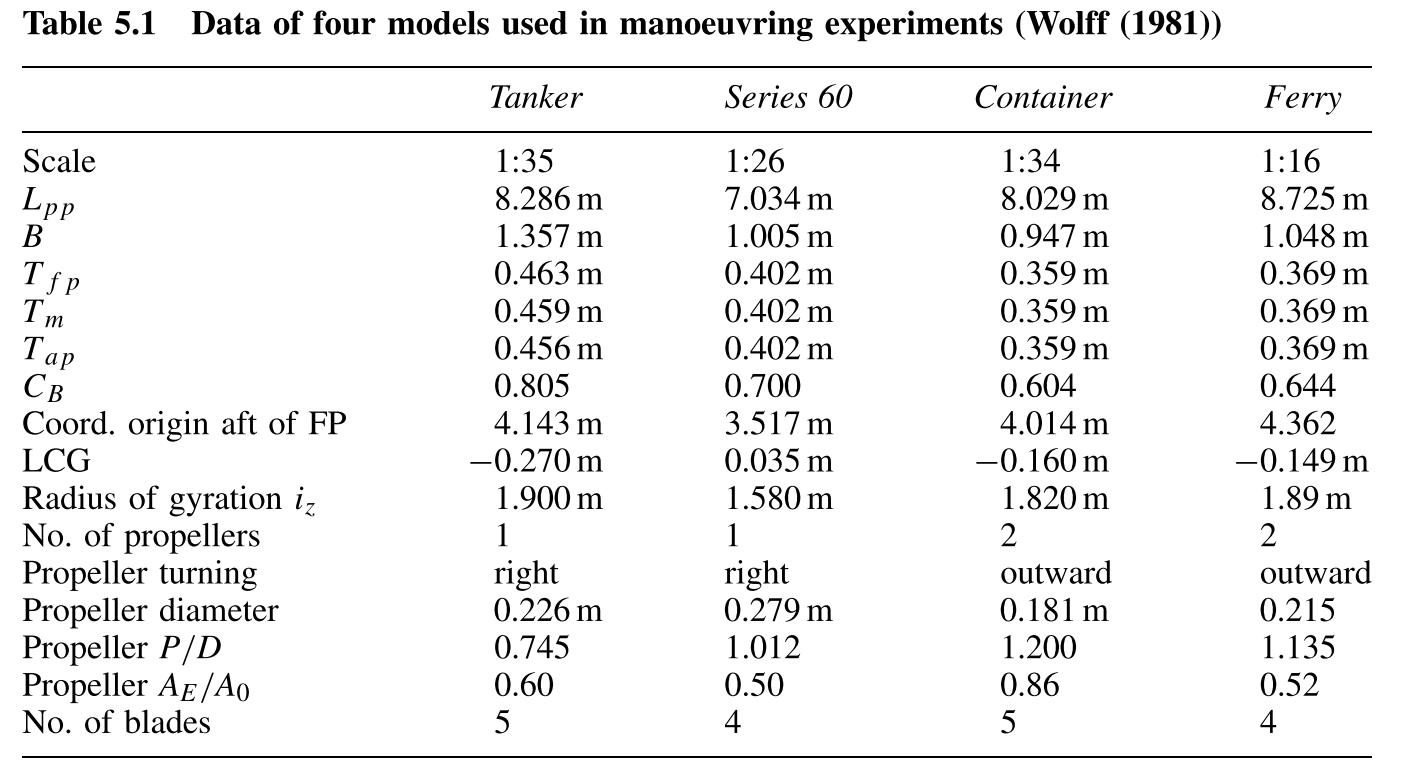
\includegraphics[width=.95\textwidth]{02_figures/betram_wolff_ratiomodel .jpg}
        \caption{Estimated value of propeller dimensions \bcitep{Bertram.2000}}
        \label{fig:betram_wolff_propellerdimensions}
\end{figure}

\subsubsection*{Calculation of shaft efficiency $\eta_S$}

The value of shaft efficiency is estimated as $\eta_S =$ \textbf{0.99} based on \bcitet{Diesel.2011} and \bcitet{Holtrop.1982}.

\subsection{Calculation of FOC}\label{sec:FOC_calc_method}

Once $R_{TOTAL}$ and $\eta_{TOTAL}$ is obtained, then the brake power of the ship $P_B$ can be calculated using \Cref{eqn:P_b}. The resulting $P_B$ will be plotted against $v_S$ to obtain a power-speed curve, then regression line will be constructed to fit the data points. Each of the BBM model will generate different prediction for SOG, the resulting equation of the regression line represents the characteristic of different BBM model. To compare the performance, the regression model from each BBM will be compared against the regression model generated from real data to assess the predictive performance of each model.\\

The FOC can be calculated using \Cref{eqn:FOC}. The information of the SFOC can be obtained from \Cref{tbl:Hammershus_Data}. Without the multiplication with operation time, $\mathcal{T}_{operation}$, The fuel consumption of the fuel in $T/h$ can be obtained by dividing the value by \textbf{$1 \cdot 10^6$}.\\  


\begin{table}
    \footnotesize
    \centering
    % \resizebox {\textwidth}{!}
    {\begin{tabular}{ p{0.1\linewidth} p{0.2\linewidth} p{0.6\linewidth}}
    \hline
    Parameter & Value & Remarks \\
    \hline
    $g$ & 9.805 $kg/ms^2$ \\
    $\rho_{sea}$ & 1025 $kg/m^3$ \\
    $\nu_{sea}$ & 0.00000118 $m^2/s$ \\
    $\rho_{air}$ & 1.25 $kg/m^3$ \\
    1 m/s & 1.9438 knots \\
    \hline
    \multicolumn{3}{l}{\textbf{Required Parameters for Holtrop-Mennen}}\\
    \hline
    $L_{WL}$ & 144.80 m & From \Cref{tbl:Hammershus_Data} \\
    $B$ & 24.50 m & From \Cref{tbl:Hammershus_Data} \\
    $T$ & 5.85 m & Assume $T_A = T_F = T$ for initial phase, otherwise use $T$ from dataset, also assume maximum draught \\
    $V$ & 13592.1413 $m^3$ & $V = C_B \cdot L_{WL} \cdot T_{MAX}$\\
    $Fr_{N}$ & 0.2417 & From \Cref{eqn:Froude_Number} \\
    $C_B$ & 0.6549 & From \Cref{eqn:Cb_Schneekluth}\\
    $C_M$ & 0.9764 & From \Cref{eqn:CM_jensen} \\
    $C_P$ & 0.6707 & From \Cref{eqn:cp_ratio}\\
    $C_{WP}$ & 0.7700 & From \Cref{eqn:cwp_Schneekluth}\\
    $\ell_{CB}$ & -0.0123 & \Cref{eqn:lcb}\\
    $A_{TR}$ & 7.3581 $m^2$ & \Cref{eqn:A_TR}\\
    $A_{BT}$ & 12.2634 $m^2$ &\Cref{eqn:A_BT}\\
    $h_B$ & 3.5100 m & Assume upper limit $h_{B} = 0.6T_F$\\
    $D$ & 4 m & Approximated from schematics \Cref{fig:Hammershus_Pict}\\
    $A_E / A_0$ & 1.135 & Value assumed from \Cref{fig:betram_wolff_propellerdimensions}\\
    $C_{stern}$ & 10 & Assume u-shaped section \Cref{eqn:c_14}\\
    \hline
    \multicolumn{3}{l}{\textbf{Optional Parameters for Holtrop-Mennen}}\\
    \hline
    $S$ & 3881.0231 $m^2$& approximated from \Cref{eqn:S_bh}\\
    $S_{APP}$ & $178.62 m^2$ & approximated from schematics \Cref{fig:Hammershus_Pict}\\
    $i_E$ & 21.6014° & \Cref{eqn:i_e}\\
    $d_{TH}$ & 2.15 m & Approximated from schematics \Cref{fig:Hammershus_Pict}\\
    \hline
    \end{tabular}}
\caption{Assumed values for power estimation}\label{tbl:assume_sea_constants}
\end{table}



\newpage
\chapter{Result and Discussion} \label{chp:result_and_discussion}

The performance of GBM will be evaluated by means of a case study using the test dataset. The test dataset comprises journey data from the whole year of 2021. The first part will focus on performance evaluation of BBM, where the trained model will be used to predict the SOG. The second part focus on the power estimation method using Holtrop-Mennen method. The output of BBM, which is the ship SOG, will be fed to the WBM to estimate the power. For further clarity regarding the methodology, the following steps are taken which are based on the proposed methodology shown in \Cref{fig:flowchart_BBM} and \Cref{fig:flowchart_WBM}. For generation of the BBM, the steps taken are:

\begin{enumerate}
    \setlength\itemsep{0em}
    \item Dataset is loaded.
    \item Identify and remove any anomalies.
    \item Remove static and unneeded features.
    \item Apply speed threshold of 5 knots.
    \item Highly correlated features are combined/removed based on physical and statistical reasoning.
    \item Impute missing values using {\tt KNNImputer}.
    \item Split the dataset into training and testing.
    \item Train the model using the whole dataset with default hyperparameter.
    \item Evaluate model performance using k-fold cross-validation.
    \item Tune the model until the best model is obtained.
    \item For the case study, the best models will be used to predict the SOG using the test dataset.
\end{enumerate}

Subsequently, for FOC calculation, the following steps are taken:

\begin{enumerate}
    \setlength\itemsep{0em}
    \item The test dataset is split into seasonal data. Summer-Fall season and Winter-Spring season which correspond to data for 6 months respectively.
    \item Impute missing values using {\tt KNNImputer}.
    \item SOG is converted to STW.
    \item Calculate calm water resistance $R_{CALM}$.
    \item Calculate added resistance due to wave $R_{AW}$.
    \item Calculate added resistance due to wind $R_{AA}$.
    \item Calculate total effective power $P_E$ using total resistance $R_{TOTAL}$.
    \item Calculate brake power $P_B$ from total efficiencies.
    \item Plot resulting regression line for Power-Speed curve from all models and actual case. 
    \item Calculate the FOC by considering the engine SFOC and operation time.
    \item Plot resulting regression line for FOC-Speed curve from all models and actual case.
    \item Evaluate the performance of the model generated from the regression lines.
\end{enumerate}

\section{Evaluation of BBM}\label{sec:BBM_tree_evaluate}

\subsection{Model Training and Selection of Optimal Parameter}\label{sec:hpo_select_train}

As mentioned in \Cref{sec:BBM_modelling}. There are 2871 data points available for training. To help narrow the search range of the hyperparameters for the tree-based model, RMSE plots against different values of hyperparameters will be performed. This method was presented in \Cref{sec:hpo}. The hyperparameter will be iteratively tuned until the best model is obtained. The result of the optimal parameter is found in \Cref{tbl:hpo_optimal}. The model training is executed using \textbf{AMD Ryzen 7 2700X, Eight-Core Processor $@$ 3.7 GHz processor with 16384 MB installed RAM}.\\


\begin{table}[ht]
    \footnotesize
    \centering
    % \resizebox {\textwidth}{!}
    {\begin{tabular}{ p{0.1\linewidth} p{0.2\linewidth}  p{0.3\linewidth} p{0.25\linewidth}}
    \hline
    Model & Training time [s] &  Optimal Hyperparameter & Search Range \\
    \hline
    DTR & 0.044 & None \\
    $\text{DTR}_{OPT}$ & 0.021  & {\tt min\_samples\_split = 7} & [2,10] \\
    &&{\tt min\_samples\_leaf = 10} & [1,10] \\
    &&{\tt max\_features = 12} & [1,12]\\
    &&{\tt max\_depth = 8} & [1,10] and [None]\\
    RFR & 4.112 & None \\
    $\text{RFR}_{OPT}$ & 3.431  & {\tt min\_samples\_split = 2} & [2,10]\\
    &&{\tt min\_samples\_leaf = 1} & [1,10]\\
    &&{\tt max\_features = 10} & [6,12]\\
    &&{\tt max\_depth = 120} & [10,200] and [None]\\
    &&{\tt n\_estimators = 100} & [100,1000]\\
    ETR & 0.944 & None \\
    $\text{ETR}_{OPT}$ & 4.390  & {\tt min\_samples\_split = 9} & [1,10]\\
    &&{\tt min\_samples\_leaf = 1} & [1,10]\\
    &&{\tt max\_features = 12} [1,12]\\
    &&{\tt max\_depth = 120} & [10,200] and [None]\\
    &&{\tt n\_estimators = 800} & [100,1000]\\
    MLR & 0.004  & None\\
    \hline
    \end{tabular}}
\caption{Optimal hyperparameter with training time of each model}\label{tbl:hpo_optimal}
\end{table}

With the default hyperparameter, RFR takes the longest training time followed by ETR and DTR. This is expected as RFR uses greedy algorithm i.e. it looks for the best possible feature when splitting the node. ETR takes significantly shorter time to train as ETR randomly select for features when splitting the node. DTR takes the shortest training time as it only generates a single tree. However, in the case of optimised model, ETR takes a longer time to train compared to RFR. This is caused by the number of trees in the optimised model which is controlled by the parameter {\tt n\_estimator}, the optimised ETR model has 800 trees in comparison to 100 trees of RFR. It is also observed that the training time of optimised DTR model is halved as pruning the tree resulted in a simpler model to train. \\

To further investigate the effect of hyperparameter optimisation, the learning curve of each tree-based model is plotted. For DTR, generated model with default parameter will result in a model that heavily overfits the training data, which is evident from the large gap between the training error and validation error which indicated a high variance as shown in \Cref{fig:learn_curve_DTR_MAE}. Regularisation i.e. parameter tuning of the DTR model helps balance between bias and variance by trading off bias for variance. This is observed from the substantial reduction in the gap between the training and validation error from \Cref{fig:learn_curve_DTR_MAE}. Additionally, the learning curve indicates that the model performance can be improved by increasing the amount of data points as the MAE continue to decrease with increasing amount of data points.\\

\begin{figure}[h]
    \centering
        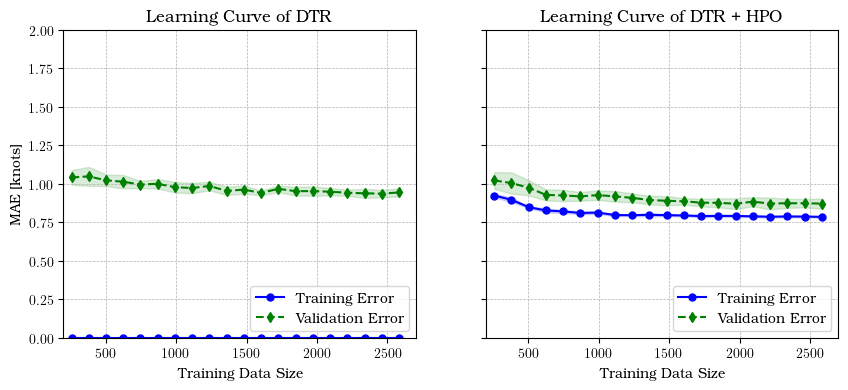
\includegraphics[width=.95\textwidth]{02_figures/learning_curve_dtr_mae.png}
        \caption{Learning curve of DTR}
        \label{fig:learn_curve_DTR_MAE}
\end{figure}

The process of hyperparameter tuning for the Random Forest Regressor (RFR) model did not show any significant improvement in model performance. This outcome aligns with the findings of  \bcitet{Kuhn.2013} and \bcitet{Hastie.2009} which was discussed in \Cref{sec:rf_theo}. The model starts to plateau at approximately 1000 data points. Furthermore, there is noticeable variance in the RFR model, which indicates that the model will have a slight tendency to overfit.\\

\begin{figure}[h]
    \centering
        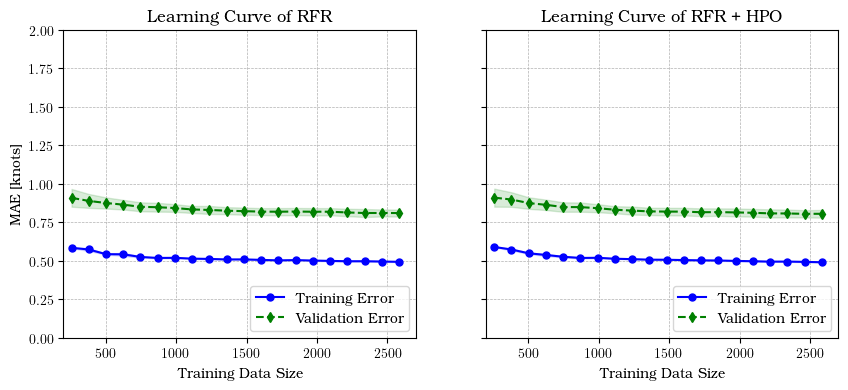
\includegraphics[width=.95\textwidth]{02_figures/learning_curve_rfr_mae.png}
        \caption{Learning curve of RFR}
        \label{fig:learn_curve_RFR_MAE}
\end{figure}

Hyperparameter tuning helps to reduce variance in the ETR model. But it does not have any major impact on model's performance. The ETR model reaches plateau beyond 1000 data points. Suggesting that adding more data points will not result in any tangible increase in model performance.\\

\begin{figure}[h]
    \centering
        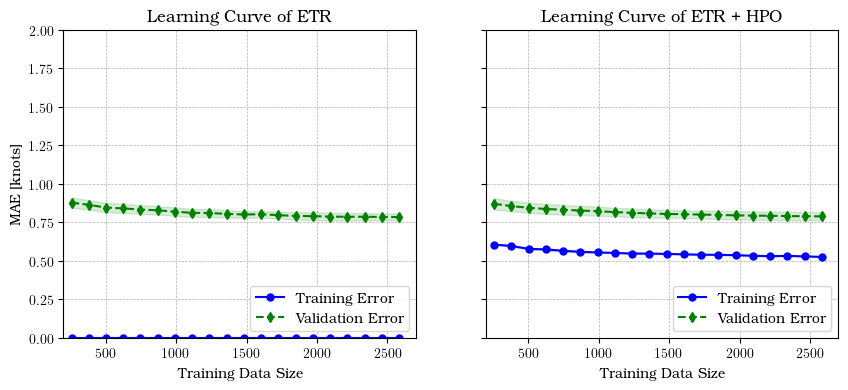
\includegraphics[width=.95\textwidth]{02_figures/learning_curve_etr_mae.png}
        \caption{Learning curve of ETR}
        \label{fig:learn_curve_ETR_MAE}
\end{figure}

\subsection{Analysis of trained model}\label{sec:BBM_model_eval}

\subsubsection{Feature Importance}\label{sec:feature_importance_bbm}

As discussed in \Cref{sec:rf_theo}, tree-based models are able to quantify the impact of each feature during the split process, this is performed using {\tt feature\_importances\_} feature in \scikit/ \bcitep{Kuhn.2013}. According to documentation by \bcitet{FabianPedregosa.2011}, it is computed as the mean and the standard deviation of accumulation of the impurity decrease within each tree i.e. total reduction of the criterion brought by a feature. Alternatively, it can be defined as how much a feature is used in each tree.\\

\begin{table}[ht]
    \scriptsize
    \centering
    \resizebox {\textwidth}{!}
    {\begin{tabular}{ p{0.15\linewidth} c| p{0.15\linewidth} c| p{0.15\linewidth} c}
    \hline
    $\text{DTR}_{OPT}$ & & $\text{RFR}_{OPT}$ & & $\text{ETR}_{OPT}$\\
    \hline
    Feature & Importance & Feature & Importance & Feature & Importance\\
    \hline
    {\tt heading} & 0.6563 & {\tt heading} & 0.4927 & {\tt cog} & 0.6410 \\
    {\tt cog} & 0.3183 & {\tt cog} & 0.4183 & {\tt heading} & 0.2707 \\
    {\tt draught} & 0.0105 & {\tt draught} & 0.0210 & {\tt truecurrentdir} & 0.0200\\
    {\tt truewinddir} & 0.0047 & {\tt curspeed} & 0.0104 & {\tt draught} & 0.0144 \\
    {\tt oceantemperature} & 0.0029 & {\tt waveperiod} & 0.0093& {\tt windwaveswellheight} & 0.0112\\
    {\tt surftemp} & 0.0025&{\tt truecurrentdir} & 0.0092 & {\tt curspeed} & 0.0110\\
    {\tt waveperiod} & 0.0019 & {\tt windwaveswellheight} & 0.0084& {\tt waveperiod} & 0.0095 \\
    {\tt truecurrentdir} & 0.0010 & {\tt surftemp} & 0.0075& {\tt windspeed} & 0.0053\\
    {\tt windwaveswellheight} & 0.0008 & {\tt truewinddir} & 0.0075& {\tt surftemp} & 0.0046 \\
    {\tt curspeed} & 0.0004 & {\tt truewavedir} & 0.0058& {\tt truewavedir} & 0.0045 \\
    {\tt windspeed} & 0.0004 & {\tt oceantemperature} & 0.0057& {\tt oceantemperature} & 0.0044\\
    {\tt truwavedir} & 0.0001 & {\tt windspeed} & 0.0056& {\tt truewinddir} & 0.0033\\
    \end{tabular}}
\caption{Feature importance of different models}\label{tbl:feature_importances}
\end{table}

The feature importances for all tree-based models shown in \Cref{tbl:feature_importances} indicated that the structure of the model is significantly influenced by the features {\tt heading} and {\tt cog}. This finding indicated that the models predicted the SOG by basis of ship movement direction i.e. heading and COG for a particular location. However, in a physical sense, it will be more insightful to consider the ship state and weather conditions that affect the prediction of the SOG.\\

\begin{figure}[h]
    \centering
        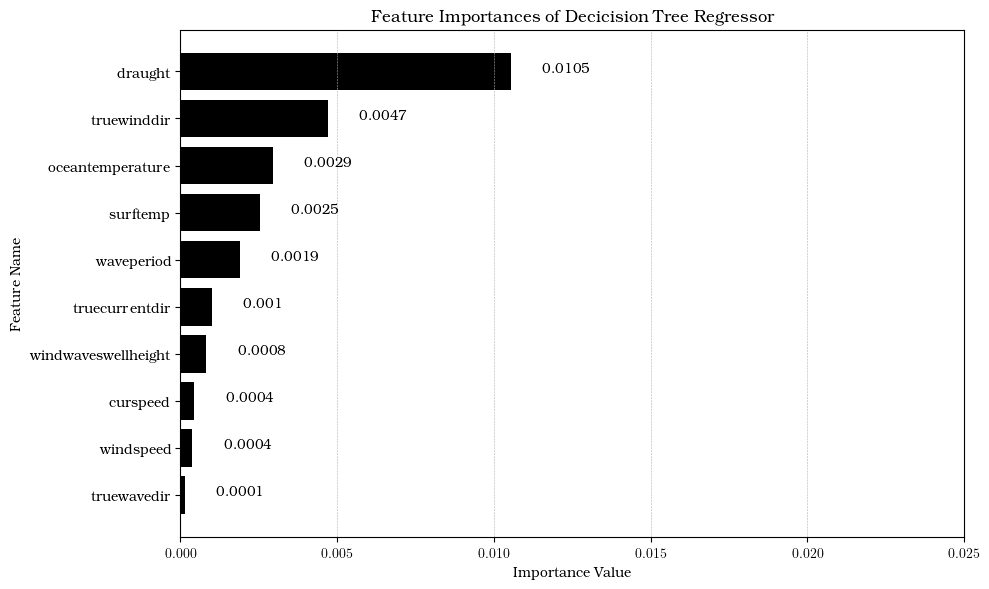
\includegraphics[width=.9\textwidth]{02_figures/dtr_ftr_importance_nodir.png}
        \caption{Feature importance of DTR}
        \label{fig:ftr_impo_dtr}
\end{figure}

Excluding ship heading and COG. The ship draught $T$ is regarded as the significant factors that affect the SOG prediction. This aligns with the theory of frictional resistance $R_F$ encountered by the ship, which is discussed in \Cref{sec:Calm_Resistance}. \Cref{eqn:R_f} is a function of wetted surface area of bare hull $S$. Deeper draught $T$ will result in more submerged area of the hull and this will consequently increase the frictional force $R_F$ of the ship. Given a constant supply of power to the ship propulsion system, the speed of the ship will decrease which is shown in \Cref{eqn:P_e}.\\

\begin{figure}[h]
    \centering
        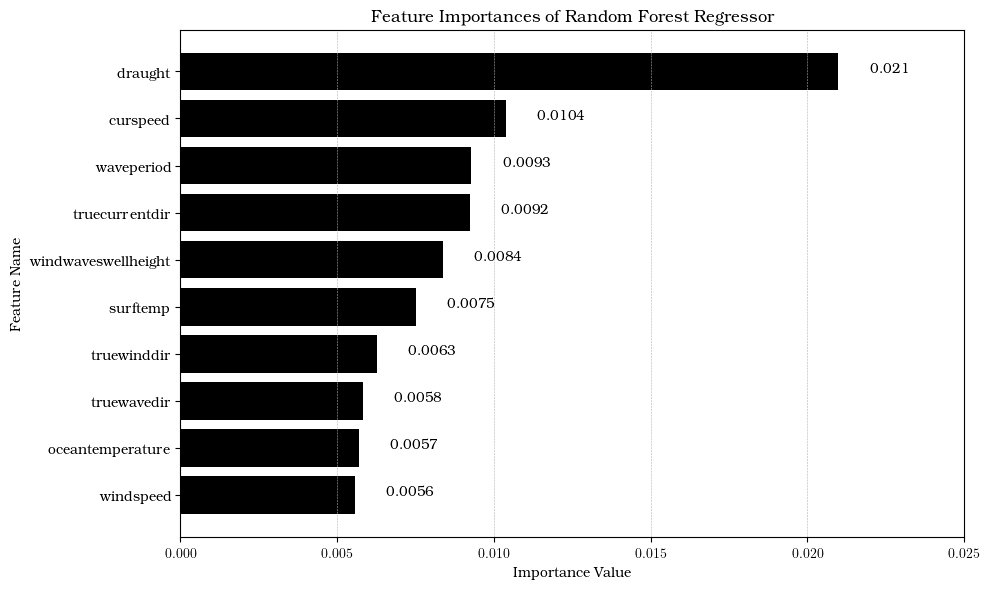
\includegraphics[width=.9\textwidth]{02_figures/rfr_ftr_importance_nodir.png}
        \caption{Feature importance of RFR}
        \label{fig:ftr_impo_rfr}
\end{figure}

\begin{figure}[h]
    \centering
        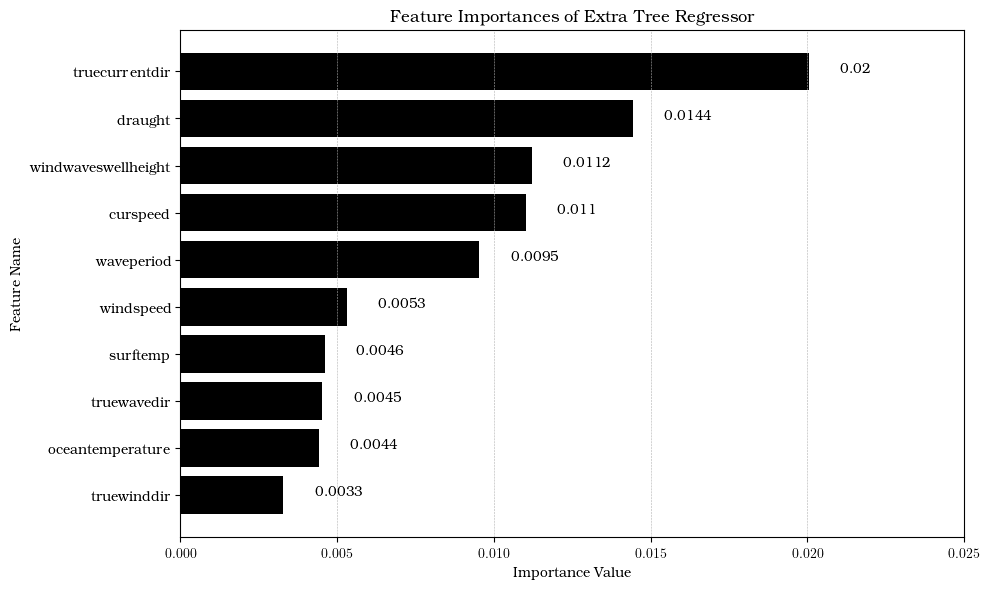
\includegraphics[width=.9\textwidth]{02_figures/etr_ftr_importance_nodir.png}
        \caption{Feature importance of ETR}
        \label{fig:ftr_impo_etr}
\end{figure}

For weather states, both RFR and ETR considered current based information such as current speed and true current direction as the most significant weather factor that affect SOG prediction. This aligns to the proposed current correction methodology presented in \Cref{sec:SOG_corr} which states that the process of current correction to convert SOG to STW requires both the magnitude and direction of the current. The next influencing feature ranked by RFR and ETR model are wave related features which are significant wave height $H_{1/3}$, true wave direction, and the wave period {\tt waveperiod}. This corresponds to the added resistance due to wave $R_{AW}$ in the calculation of total resistance $R_{TOTAL}$ encountered by the ship. The wind related features, which are wind speed and its true direction, corresponds to added resistance due to wind force $R_{AA}$ and is found to be the least influential in SOG prediction in RFR and ETR model.\\

Based on the behaviour of the Random Forest Regressor (RFR) and Extra Trees Regressor (ETR) models, it can be inferred that waves have a more significant impact on the Speed Over Ground (SOG) compared to the influence of wind during the ship's journey. However, the Decision Tree Regressor (DTR) model demonstrates that temperature-related features, such as Sea Surface Temperature (SST) and air temperature above the ocean, have a more significant effect on SOG predictions than most other features. While the importance of temperature is not as pronounced as in RFR or ETR models, this finding suggests that the ship's SOG is implicitly influenced by the time of the travel or the season in which the journey takes place.\\

\subsubsection*{Structure of generated tree-based model}

\begin{figure}[h]
    \centering
        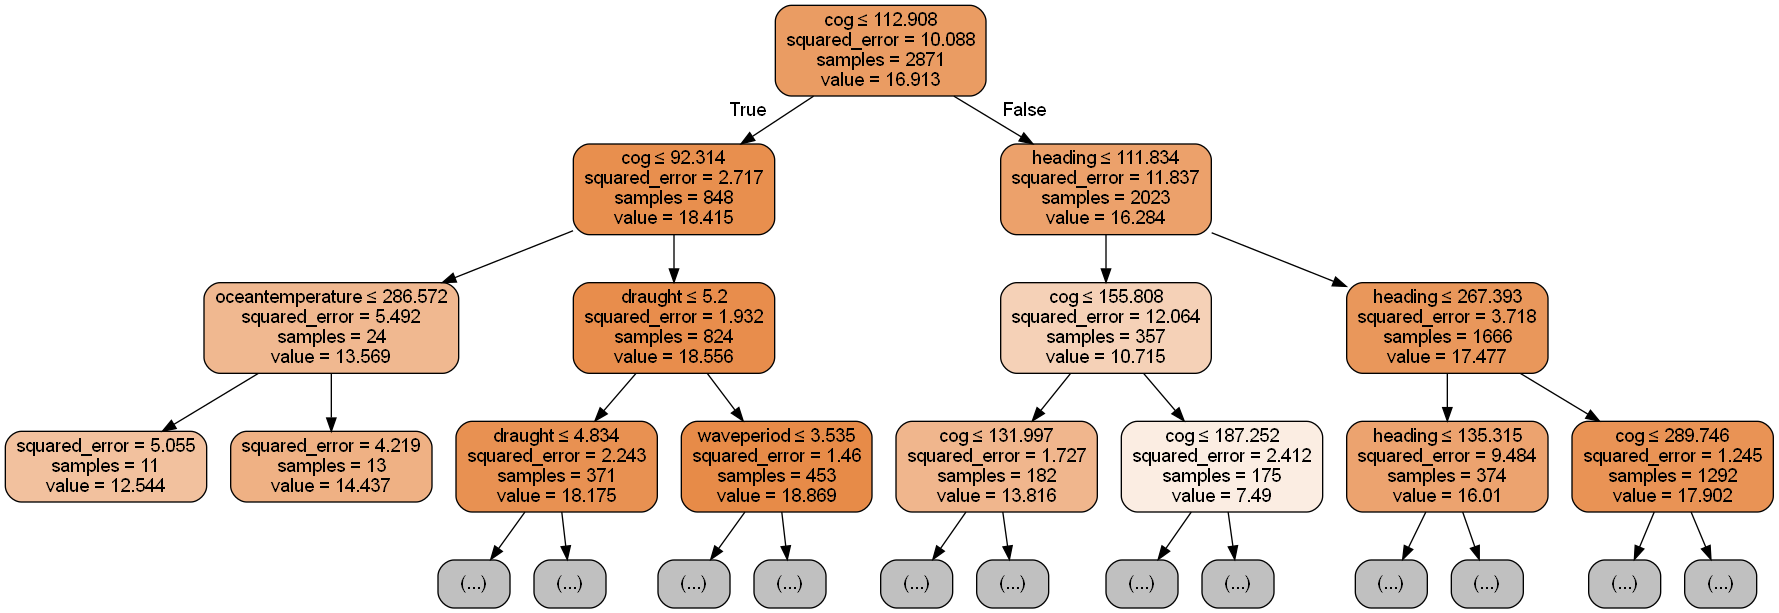
\includegraphics[width=.9\textwidth]{02_figures/dtr_mod_1tree.png}
        \caption{Partial structure of DTR}
        \label{fig:dtr_tree_hpov}
\end{figure}

To understand the effect of hyperparameter optimisation and feature importance, analysis on the structure of generated tree-based models will be performed. The shading in the nodes indicated the likelihood of the decision, where darker shading means greater likelihood. Each node indicates information on the splitting feature with the threshold, the SSR score, amount of samples and the predicted SOG value. Even after pruning, the tree can grow relatively large, therefore, the illustration of the trees is limited to a depth of {\tt max\_depth = 3} and for RFR and ETR, only the illustration of a specific tree in the forest will be shown.\\

The structure of the optimised decision tree shown in \Cref{fig:dtr_tree_hpov} show the effect of regularisation at the leaf node. For example, the leaf nodes that splits the feature, ocean temperature, does not completely minimise the SSR. This is caused by the hyperparameter tuning of the minimum samples at the leaf node, which was set at {\tt min\_samples\_leaf = 10}, splitting these nodes further will cause subsequent leaf nodes that have less than 10 samples. In this figure, the significance of COG and ship heading can be clearly seen, as it is used to split many of the internal nodes in the tree.\\

\begin{figure}[h]
    \centering
        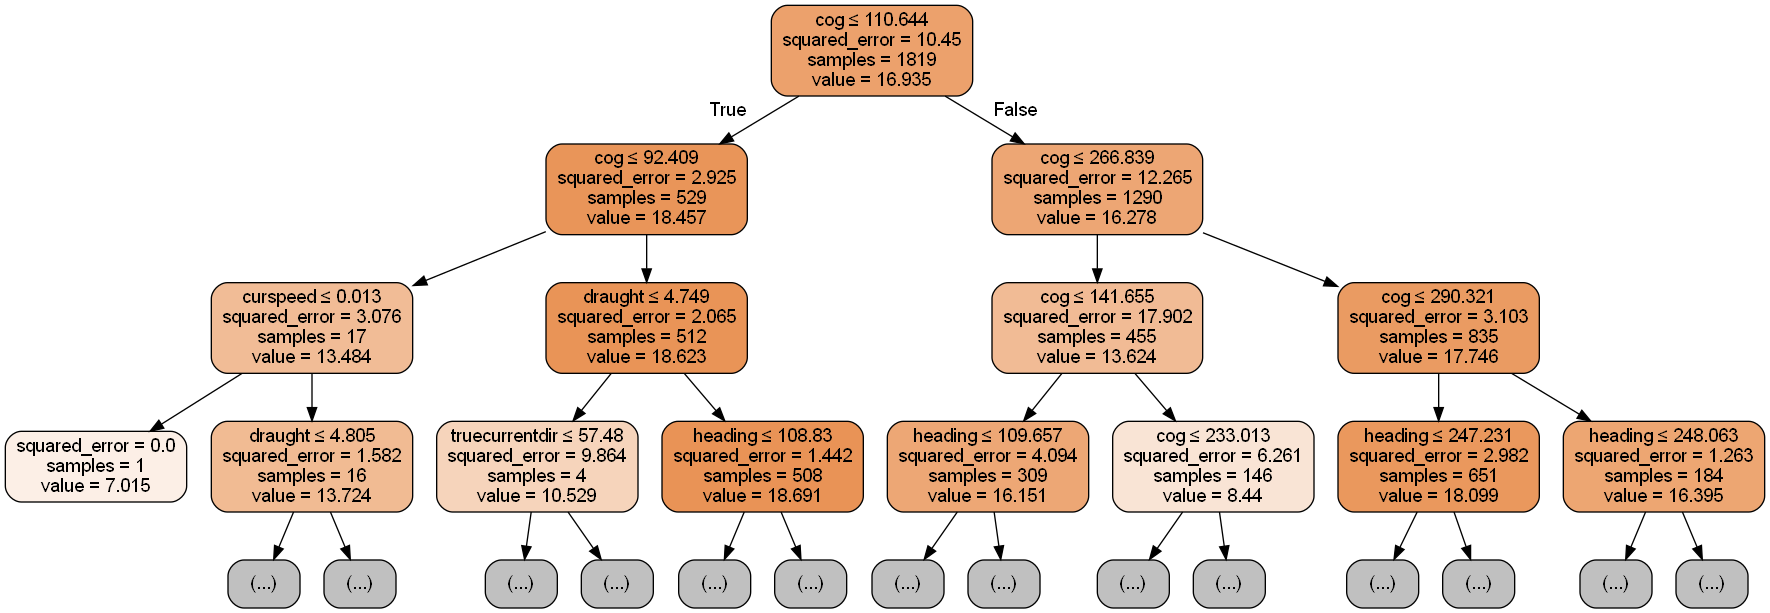
\includegraphics[width=.9\textwidth]{02_figures/rfr_mod_it1.png}
        \caption{Partial structure of {\tt n\_estimators = 1} for RFR}
        \label{fig:rfr_tree1_hpov}
\end{figure}

The illustration of the first RFR tree is shown in \Cref{fig:rfr_tree1_hpov}. Similar to DTR, both COG and ship heading are regarded as the best features to split the internal node. In this tree of the forest, the effect of allowing full tree growth can be observed in the leaf node when splitting the feature current speed. This tree is able to minimise the SSR to its possible minimum value, and the leaf node cannot be further split as there are no more available samples. The effect of bagging for the dataset and feature selection in RFR can also be observed in this tree as the structure of this tree is completely different to DTR tree shown in \Cref{fig:dtr_tree_hpov}.\\

\begin{figure}[h]
    \centering
        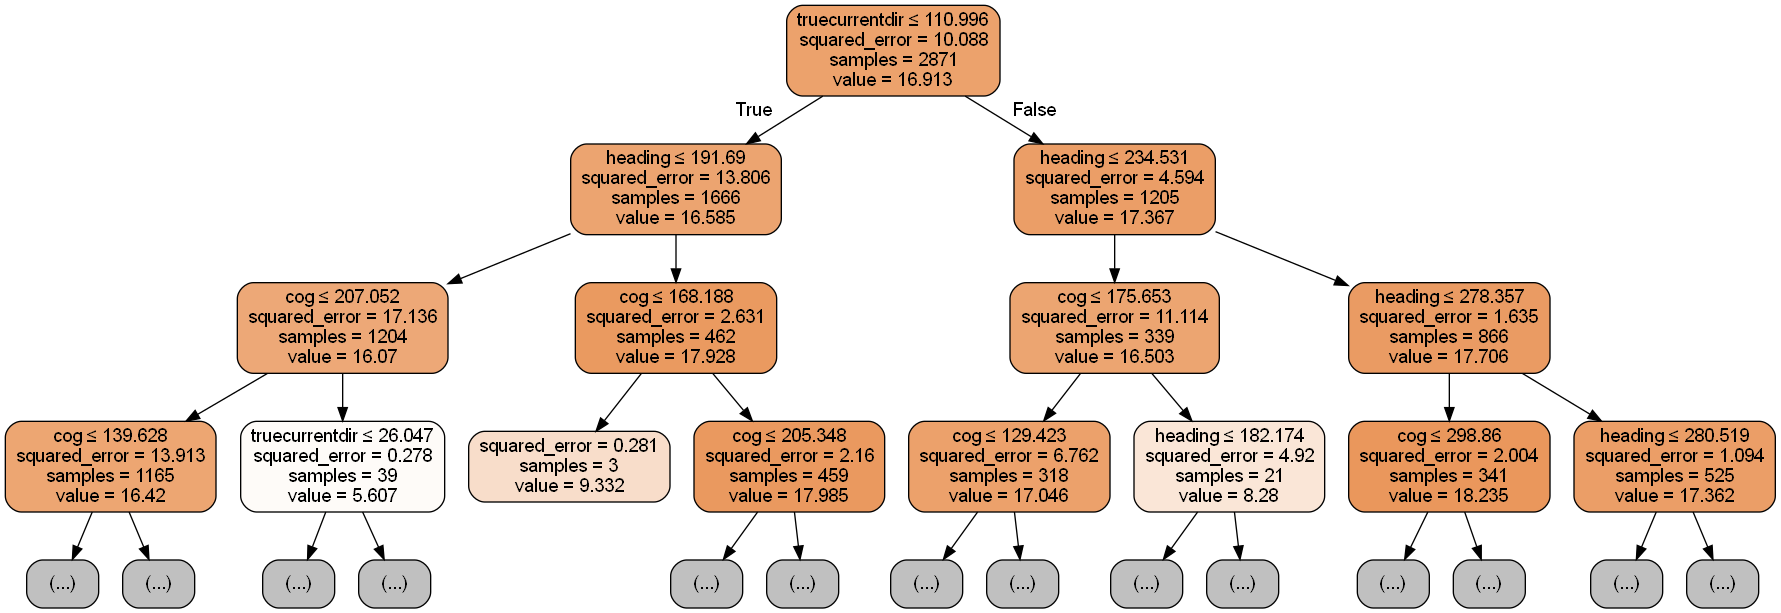
\includegraphics[width=.9\textwidth]{02_figures/etr_mod_it1.png}
        \caption{Partial structure of {\tt n\_estimators = 1} for ETR}
        \label{fig:etr_tree1_etr}
\end{figure}
The random selection of the feature to split of ETR can be seen in the structure of the first tree in an ETR in \Cref{fig:etr_tree1_etr}. Since both DTR and RFR uses greedy algorithm, i.e. it finds the possible splits which minimise the cost function, both model selected COG as the parent node. However, the randomness in feature selection of ETR can be clearly observed in this illustration, the model selects the true current direction as the parent node. Also, due to regularisation of ETR, the leaf node when splitting COG does not completely minimise the SSR. The split is not allowed since it does not meet the tuning criteria of {\tt min\_samples\_split = 9}.\\ 

\subsubsection{Evaluation of k-fold cross-validation}\label{sec:bbm_kfold_perf_eval}

The performance of the model is evaluated using the training dataset using 10-fold cross validation. This means that the training will be repeated 10 times using 9 of the folds as training dataset, the remaining fold will be used as validation dataset. The results from k-folding validation process is shown in \Cref{fig:k_fold_validation_result}. The inside (orange) line represents the median i.e. $50\%$ of the score in k-folding. The top and the bottom of the box correspond to the first i.e. $25\%$ and third quartile i.e. $75\%$ respectively. The whiskers represent the lowest data point within the 1.5 Interquartile Range (IQR) of the lowest quartile and the highest point of data within 1.5 IQR of the upper quartile. The mean is indicated by the (green) triangle. Data points beyond the whisker range is shown as hollow circle.\\
\begin{figure}[ht]
    \centering
  
    \begin{minipage}{0.45\textwidth}
      \centering
      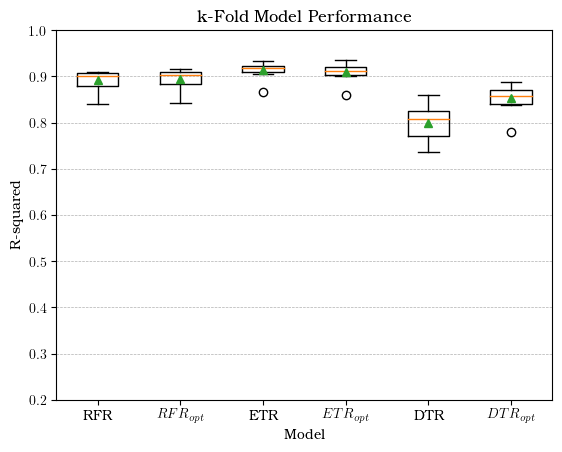
\includegraphics[width=\textwidth]{02_figures/kfold_r2_opt.png}
    \end{minipage}
    \hfill
    \begin{minipage}{0.45\textwidth}
      \centering
      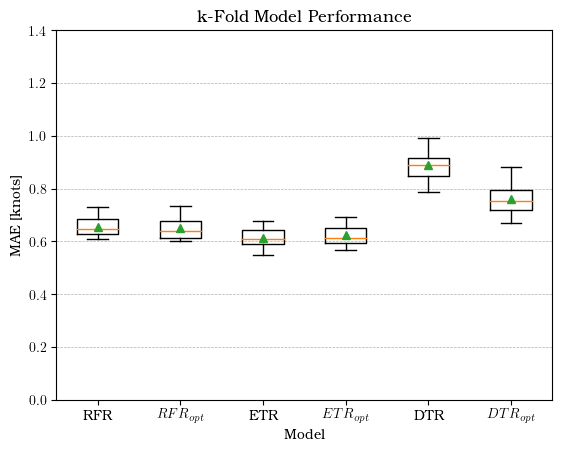
\includegraphics[width=\textwidth]{02_figures/kfold_mae_opt.png}
    \end{minipage}
  
    \vspace{0.5cm} % Adjust the vertical space between rows
  
    \begin{minipage}{0.45\textwidth}
      \centering
      \includegraphics[width=\textwidth]{02_figures/kfold_rmse_opt.png}
    \end{minipage}
    \hfill
    \begin{minipage}{0.45\textwidth}
      \centering
      \includegraphics[width=\textwidth]{02_figures/kfold_mad_opt.png}
    \end{minipage}
  
    \caption{Evaluation of k-fold cross-validation for different performance indices}
    \label{fig:k_fold_validation_result}
  \end{figure}

The box plots indicated that ETR achieved the best performance, the model is able to achieve $R^2$ score of around $91\%$ and MAE of around 0.6 knots. The model is also relatively stable, which is indicated by the narrow box plots. RFR also achieved similar performance, achieving $R^2$ score of about $89\%$ and MAE of approximately 0.65 knots. As illustrated previously in \Cref{fig:learn_curve_ETR_MAE} and \Cref{fig:learn_curve_RFR_MAE}, optimisation does not yield any significant improvement in model performance. DTR greatly benefits from regularisation, the model achieves an increase of about $5\%$ for the $R^2$ score and a reduction from about 0.89 knots to 0.76 knots for the MAE, similar improvements can be observed in both RMSE and MAD. To summarise, all tree-based models exhibited good fit performance with mean/median $R^2$ scores above $80\%$. However, the value of RMSE is quite significant, the values lies between 1.00 to 1.20 knots across the models. To put this into scale, the mean SOG of the training data is at 16.91 knots as shown in \Cref{tbl:dataset_descriptive_pretraining}.\\  

\subsection{Performance evaluation of BBM}\label{sec:Perf_eval_BBM}

\subsubsection{Analysing the testing dataset}\label{sec:testing_data_analysis}

Once the best model is determined, the model will be tested against the testing dataset. The testing dataset correspond to 957 datasets across 2021, the dataset for the whole year is indicated as $DS_{year}$. To investigate the effect of data points on the model performance, the dataset is split into two seasons, $DS_{summer}$, which corresponds to summer datasets and it represents data between May 2021 and October 2021, there are 454 data points between this period. Winter dataset, $DS_{winter}$, correspond to testing datasets between January 2021 and April 2021 as well as November 2021 and December 2021 which correspond to 503 data points. Any missing values which are present in the testing dataset will be using {\tt KNNImputer}.\\

\begin{table}[h]
    \footnotesize
    \centering
    % \resizebox {\textwidth}{!}
    {\begin{tabular}{ p{0.21\linewidth} c c c c c c c c }
    \hline
    Features & Count & Mean & Std. & Min & 25\% & 50\% & 75\% & Max \\
    \hline
    \textbf{{\tt sog}} & 957.00 & 16.99 & 3.10 & 5.10 & 16.68 & 18.05 & 18.72 & 21.00\\
    \hline
    {\tt cog} & 957.00 & 196.73 & 86.72&	56.02 & 102.32& 185.22& 282.18& 319.85\\ 
    {\tt heading} & 957.00 & 188.30&	89.17&	63.49&	100.86&	124.24&	279.38&	308.04\\
    {\tt draught} & 957.00 & 5.23 & 0.19& 4.74& 5.11& 5.29& 5.38&5.66\\
    {\tt windspeed} & 957.00 & 6.45 & 3.04 & 0.40 & 4.11 & 6.13 &	8.21 & 15.85\\
    {\tt oceantemperature} & 957.00 & 282.28 & 6.48 & 267.25& 276.80& 281.91& 288.42& 295.70 \\
    {\tt waveperiod} & 957.00 & 3.70 & 0.88 & 1.67 & 3.06& 3.62& 4.22& 7.01\\
    {\tt surftemp} & 957.00 &283.22& 5.72& 273.15& 277.98& 282.73& 288.82 &294.93\\
    {\tt windwaveswellheight} &  957.00 & 0.77 & 0.54 & 0.08 &0.37 &	0.66 &	0.94 &  3.24  \\
    {\tt curspeed} & 957.00 &0.09 & 0.07& 0.00 & 0.05& 0.07 & 0.13 & 0.50\\
    {\tt truewinddir} & 957.00 & 91.39 & 56.23 &	0.03 & 38.80 &	95.25 & 142.83 & 179.86\\
    {\tt truecurrentdir} & 957.00 & 90.75 & 57.76 & 0.26 & 31.52 & 90.44 & 144.65 & 179.95 \\
    {\tt truewavedir} & 957.00 & 86.90 & 55.74& 0.06& 36.24 & 81.54 & 138.04 & 179.81 \\
    \hline
    \end{tabular}}
\caption{Descriptive statistics of $DS_{year}$}\label{tbl:testyear_dataset_descriptive}
\end{table}

\begin{table}[h]
    \footnotesize
    \centering
    % \resizebox {\textwidth}{!}
    {\begin{tabular}{ p{0.21\linewidth} c c c c c c c c }
    \hline
    Features & Count & Mean & std & Min & 25\% & 50\% & 75\% & Max \\
    \hline 
    \textbf{{\tt sog}} & 454.00 & 17.26 & 2.91 & 5.22 & 16.74 & 18.17 & 18.95 & 21.01\\
    \hline
    {\tt cog} & 454.00 & 196.06 & 87.55 &  56.02 & 102.80 & 182.79 & 282.03 & 319.85 \\ 
    {\tt heading} & 454.00 & 188.08 & 89.02 &  63.49 & 100.75 & 124.68 & 278.07 & 303.30 \\
    {\tt draught} & 454.00 &   5.30 &  0.17 &   4.74 &   5.20 &   5.29 &   5.38 &   5.66 \\
    {\tt windspeed} & 454.00 &   6.64 &  3.33 &   0.40 &   4.08 &   6.30 &   8.71 &  15.85 \\
    {\tt oceantemperature} & 454.00 & 285.59 &  5.90 & 269.27 & 282.90 & 286.70 & 290.04 & 295.70 \\
    {\tt waveperiod} & 454.00 & 3.73 &  0.99 &   2.02 &   2.95 &   3.60 &   4.36 &   7.01 \\
    {\tt surftemp} & 454.00 & 286.33 &  5.10 & 274.75 & 283.05 & 287.58 & 290.18 & 294.93 \\
    {\tt windwaveswellheight} & 454.00 &   0.82 &  0.63 &   0.08 &   0.36 &   0.67 &   1.02 &   3.24 \\
    {\tt curspeed} & 454.00 &   0.10 &  0.07 &   0.00 &   0.04 &   0.07 &   0.13 &   0.50 \\
    {\tt truewinddir} & 454.00 &  90.94 & 58.05 &   0.60 &  38.40 &  89.86 & 145.86 & 179.58 \\
    {\tt truecurrentdir} & 454.00 &  83.65 & 59.53 &   0.26 &  26.68 &  70.51 & 143.73 & 179.33 \\
    {\tt truewavedir} & 454.00 &  88.06 & 59.52 &   0.09 &  33.00 &  82.18 & 145.69 & 179.81 \\
    \hline
    \end{tabular}}
\caption{Descriptive statistics of $DS_{summer}$}\label{tbl:testsummer_dataset_descriptive}
\end{table}

\begin{table}[h]
    \footnotesize
    \centering
    % \resizebox {\textwidth}{!}
    {\begin{tabular}{ p{0.21\linewidth} c c c c c c c c }
    \hline
    Features & Count & Mean & std & Min & 25\% & 50\% & 75\% & Max \\
    \hline
    \textbf{{\tt sog}} & 503.00 & 16.75 & 3.24 & 5.10 & 16.59 & 17.98 & 18.61 & 20.70\\
    \hline
    {\tt cog} & 503.00 & 197.33 & 86.06 &  80.81 & 102.25 & 187.56 & 282.63 & 307.92 \\
    {\tt heading} & 503.00 & 188.50 & 89.39 &  89.22 & 100.87 & 123.92 & 280.05 & 308.04 \\
    {\tt draught} & 503.00 &   5.16 &  0.18 &   4.76 &   5.02 &   5.20 &   5.29 &   5.65 \\
    {\tt windspeed}& 503.00 &   6.28 &  2.76 &   0.43 &   4.12 &   6.05 &   8.01 &  14.35 \\
    {\tt oceantemperature} & 503.00 & 279.29 &  5.44 & 267.25 & 275.74 & 278.22 & 281.25 & 292.72 \\
    {\tt waveperiod} & 503.00 & 3.67 &  0.76 &   1.67 &   3.16 &   3.62 &   4.14 &   5.98 \\
    {\tt surftemp} & 503.00 & 280.41 &  4.71 & 273.15 & 277.23 & 278.68 & 282.68 & 292.85 \\
    {\tt windwaveswellheight} & 503.00 &   0.73 &  0.45 &   0.08 &   0.40 &   0.66 &   0.90 &   2.43 \\
    {\tt curspeed} & 503.00 &   0.09 &  0.07 &   0.00 &   0.05 &   0.08 &   0.12 &   0.42 \\
    {\tt truewinddir} & 503.00 &  91.81 & 54.61 &   0.03 &  39.66 &  97.92 & 140.20 & 179.86 \\
    {\tt truecurrentdir} & 503.00 &  97.16 & 55.40 &   1.44 &  41.92 & 102.12 & 145.34 & 179.95 \\
    {\tt truewavedir} & 503.00 &  85.86 & 52.13 &   0.06 &  39.44 &  81.22 & 132.49 & 178.30 \\
    \hline
    \end{tabular}}
\caption{Descriptive statistics of $DS_{winter}$}\label{tbl:testwinter_dataset_descriptive}
\end{table}

\subsubsection{Result and Discussion of BBM}\label{sec:result_discussion_BBM}

The results of SOG prediction of optimised the tree-based models is summarised in \Cref{tbl:testing_dataset_sog_result}. Each model is tested against 3 different testing datasets, the yearly dataset $DS_{year}$, summer dataset, $DS_{summer}$ and winter dataset $DS_{winter}$. The performance of the tree models is compared against Multiple Linear Regressor (MLR) model.

\begin{table}[ht]
    % \footnotesize
    \small
    \centering
    % \resizebox {\textwidth}{!}
    {\begin{tabular}{ l l c c c c c c }
    \hline
    Model & Dataset & $R^2$ & expVar & MAE & RMSE & MAD & MAPE \\
    & & [$\%$] & [$\%$] & [$kn$] & [$kn$] & [$kn$] & [$\%$]  \\ 
    \hline
    $\text{DTR}_{OPT}$ & $DS_{year}$ & 86.72 & 86.75 & 0.714 & 1.129  & 0.479 & 4.96  \\
    & $DS_{winter}$ & 88.51 & 88.61 & 0.690 & 1.100 & 0.441 & 4.95 \\
    & $DS_{summer}$ & 84.04 & 84.05 & 0.741 & 1.161 & 0.520 & 4.97 \\
    $\text{RFR}_{OPT}$ & $DS_{year}$  & 90.13 & 96.16 & 0.629 & 0.973 & 0.419 & 4.29 \\
    & $DS_{winter}$ & 93.40 & 93.52 & 0.549 & 0.833 & 0.374 & 3.96 \\
    & $DS_{summer}$ & 85.48 & 85.48 & 0.696 & 1.108 & 0.455 & 4.66 \\
    $\text{ETR}_{OPT}$ & $DS_{year}$ & 91.09 & 91.91 & 0.582 & 0.882 & 0.398 & 3.96 \\
    & $DS_{winter}$ & \textbf{94.55} & \textbf{94.63} & \textbf{0.532} & \textbf{0.756} & \textbf{0.394} & \textbf{3.72} \\
    & $DS_{summer}$ & 88.11 & 88.13 & 0.637 & 1.002 & 0.409 & 4.23 \\
    MLR & $DS_{year}$ & 69.61 & 69.67 & 1.147 & 1.707 & 0.924 & 7.73 \\
    & $DS_{winter}$ & 68.08 & 68.08 & 1.135 & 1.831 & 0.880 & 8.04 \\
    & $DS_{summer}$ & 71.21 & 71.56 & 1.160 & 1.560 & 0.949 & 7.39 \\
    \hline
    \end{tabular}}
\caption{Performance indices for different modelling approach and different testing datasets}\label{tbl:testing_dataset_sog_result}
\end{table}

From \Cref{tbl:testing_dataset_sog_result}, it can be observed that all tree-based model is able to achieve good prediction results on different testing datasets. Generally, all tree-based models obtained $R^2$ score above $80\%$ and perform better when using the $DS_{winter}$ datasets. All tree-based models offer significant improvement from MLR. Among the tree-based model, ETR presented the best SOG prediction across different datasets, followed by RFR and DTR.\\ 

\begin{table}[h]
    \footnotesize
    \centering
    % \resizebox {\textwidth}{!}
    {\begin{tabular}{ l l c c c c c c c c }
    \hline
    Model & Dataset & Count & Mean & std & Min & 25\% & 50\% & 75\% & Max \\
    \hline
    \textbf{{Actual}} & $DS_{year}$ & 957.00 &  16.99 &   3.10 & 5.10 &  16.68 &  18.05 &  18.72 &  21.01 \\
    & $DS_{winter}$ & 503.00 &  16.75 &   3.24 & 5.10 &  16.59 &  17.98 &  18.61 &  20.70 \\
    & $DS_{summer}$ & 454.00 &  17.26 &   2.91 & 5.22 &  16.74 &  18.17 &  18.95 &  21.01 \\
    \hline
    $\text{DTR}_{OPT}$ & $DS_{year}$ & 957.00 &  17.04 &   2.91 & 5.36 &  16.58 &  18.11 &  18.66 &  20.00 \\
    & $DS_{winter}$ & 503.00 &  16.85 &   3.06 & 5.36 &  16.58 &  17.86 &  18.58 &  19.98 \\
    & $DS_{summer}$ & 454.00 &  17.25 &   2.73 & 5.64 &  16.58 &  18.15 &  18.91 &  20.00 \\
    \hline
    $\text{RFR}_{OPT}$ & $DS_{year}$ & 957.00 &  17.04 &   2.89 & 5.37 &  16.71 &  18.11 &  18.70 &  20.22 \\
    & $DS_{winter}$ & 503.00 &  16.86 &   3.04 & 5.37 &  16.70 &  18.02 &  18.60 &  19.74 \\
    & $DS_{summer}$ & 454.00 &  17.25 &   2.72 & 5.81 &  16.74 &  18.20 &  18.77 &  20.22 \\
    \hline
    $\text{ETR}_{OPT}$ & $DS_{year}$ & 957.00 &  17.03 &   2.87 & 5.39 &  16.67 &  18.05 &  18.65 &  19.96 \\
    & $DS_{winter}$ & 503.00 &  16.84 &   3.04 & 5.39 &  16.65 &  17.96 &  18.56 &  19.87 \\
    & $DS_{summer}$ & 454.00 &  17.23 &   2.66 & 5.96 &  16.71 &  18.18 &  18.75 &  19.96 \\
    \hline
    \end{tabular}}
\caption{Descriptive statistics of SOG Prediction}\label{tbl:SOG_pred_descriptive}
\end{table}

\begin{figure}[ht]
\centering

\begin{minipage}[b]{0.32\textwidth}
    \centering
    \includegraphics[width=\textwidth]{02_figures/sog_pred_year.png}
    % \caption{Caption for Picture 1.}
    \label{fig:boxplot_dsyear}
\end{minipage}%
\hfill
\begin{minipage}[b]{0.32\textwidth}
    \centering
    \includegraphics[width=\textwidth]{02_figures/sog_pred_winter.png}
    % \caption{Caption for Picture 2.}
    \label{fig:boxplot_dswinter}
\end{minipage}%
\hfill
\begin{minipage}[b]{0.32\textwidth}
    \centering
    \includegraphics[width=\textwidth]{02_figures/sog_pred_summer.png}
    % \caption{Caption for Picture 3.}
    \label{fig:boxplot_dssummer}
\end{minipage}

\caption{SOG distribution for $DS_{year}$, $DS_{winter}$ and $DS_{summer}$}
\label{fig:boxplot_sogPred_overall}
\end{figure}  

To gain more insight to the predictive performance, descriptive statistics of the SOG prediction is provided \Cref{tbl:SOG_pred_descriptive}. The results implied that the model is not able to capture information on the lower end of the ship speed across the different datasets. This is possibly caused by low number of data points that represent lower end of the SOG speed, this is evident from the boxplots of the different datasets shown in \Cref{fig:boxplot_sogPred_overall} and the plot actual against predicted SOG shown in \Cref{fig:pred_vs_act_SOG}. The sparsity of data points in lower SOG range is clearly indicated in \Cref{fig:pred_vs_act_SOG}.\\

\begin{figure}[h]
    \centering
        \includegraphics[width=.9\textwidth]{02_figures/pred_vs_act_all_tree.png}
        \caption{Actual vs Predicted SOG for DTR, RFR and ETR}
        \label{fig:pred_vs_act_SOG}
\end{figure}

Both the descriptive statistics and boxplots implied that the data points distributions are skewed towards the higher end of SOG, with the majority of data points concentrated within approximately 16.5 knots for the first quartile and 19 knots for the third quartile across all datasets. The lowest data point within the $1.5 \cdot \text{IQR}_{LOW}$ distribution lies at approximately 13.6 knots, which is indicated by the lower whisker in the boxplot. Although the boxplots may suggest that data points beyond the whisker are outliers, this is not the case, as these points should represent ship journeys at low speeds. The limited representation of low-speed data points contributes to the model's inability to effectively predict SOG at the lower end of the range.\\

This may explain the relatively high value of RMSE for all models as it treats the data points for low SOG as outliers, as previously discussed in \Cref{sec:perf_metrics}, RMSE are more sensitive to outliers in comparison to both MAE and MAD, making it less representative in this case study which results in MAE and MAD being the more suitable error evaluation metrics to be used in this case study. Furthermore, the high scores of $R^2$ and explained Variance can be attributed to the models' ability to predict SOG values that lie within the whiskers of the box plots, indicating good prediction performance within those ranges.\\

There are two possible solutions to address this problem:\\ 

\textbf{Increasing the number of data points in lower SOG range}: this is the apparent solution to this problem, this will help widen the IQR of the boxplot, and it should not misclassify data points in lower range of the SOG as outliers. This could also potentially improve the results of performance indices such as $R^2$ and RMSE. However, \emph{specific to this case study}, this may not be possible as the limitation of T-AIS shown in \Cref{fig:aiscoverage}. The ship will decrease its speed as it approach a port, or it will gradually increase its speed as it leaves a port. However, T-AIS coverage around the port of K{\o}ge and R{\o}nne are either problematic i.e. transmission reception rate at around $50\%$ to $80\%$ or poor i.e. transmission rate less than $50\%$. This may prove to be challenging to as it may not be possible to increase the number of data points around these regions.\\ 

\textbf{Reducing skew of the data}: \bcitet{Gkerekos.2019} applied the outlier rejection formula which uses the formula $\mu \pm 3\sigma$, where $\mu$ is the mean and $\sigma$ is the standard deviation. Assuming normal distribution, $99.7\%$ of the normal data should be within this range. Another method of reducing the skew is by applying higher threshold of the minimum SOG value. While this may help reduce overall errors and improve model fit, this approach will negate the capability of the model to make prediction when the ship is sailing at a reduced speed. Careful consideration of the trade-offs is required when selecting the most appropriate approach.\\

\section{Evaluation of WBM}\label{sec:WBM_perf_eval}

\subsection{Analysis of WBM}\label{sec:Power_estimation_actual}

The findings of power estimation using the Holtrop-Mennen method are presented in \Cref{tbl:PB_act_descriptive_yr} and \Cref{fig:hist_resistance_power_yr}. To gain insights into the overall model behavior, the analysis is conducted using the actual data from the $DS_{year}$ datasets.To facilitate a better interpretation of the scale of magnitude, the histograms for the resistance components utilize identical scaling.\\

For calm water resistance $R_{CALM}$, the largest portion is attributed to the frictional resistance $R_F$, which accounts for approximately $39\%$ of $R_{TOTAL}$ when considering the mean. Following this, the wave-making and breaking resistance $R_W$ contribute around $21\%$. Subsequently, the bulbous bow resistance $R_{B}$ accounts for approximately $16\%$, the correlation resistance $R_{A}$ around $10\%$, and the appendage resistance $R_{APP}$ at approximately $8\%$. The transom resistance $R_{TR}$ has a relatively negligible impact on $R_{CALM}$, accounting for only about $1\%$.\\

Reagrding the added resistance due to surrounding weather conditions, the contribution of added resistance due to wind $R_{AA}$ are noticeable and add a significant amount to the total resistance $R_{TOTAL}$. In contrast, the added resistance due to waves $R_{AW}$ is comparatively negligible. This behavior can be explained by referring to \Cref{tbl:testyear_dataset_descriptive}, the sea conditions along the ship's sailing path are relatively calm, with a mean significant wave height $H_{1/3}$ of $0.77 m$ and a mean wind speed of $6.45 m/s$. By only considering the mean, the combined additional resistance to weather conditions only makes up to about $3.5\%$ of the total resistance.\\

These results further validate the BBM's ranking of ship draught $T$ as the most significant physical factor that affect the ship speed. The WBM also further confirm the BBM suggestion that wave resistance might have a more significant impact on the speed compared to wind resistance. This is evident from the maximum achievable resistance of $R_{AA}$ and $R_{AWL}$ shown in \Cref{tbl:PB_act_descriptive_yr}. However, over the journey, the mean of $R_{AWL}$ is significantly lower, primarily due to the condition in \Cref{eqn:stawave1}, which only consider the wave correction force within $\pm 45$° off bow.\\  

\begin{table}[h]
    \footnotesize
    \centering
    % \resizebox {\textwidth}{!}
    {\begin{tabular}{ p{0.04\linewidth} p{0.03\linewidth} c c c c c c c c }
    \hline
    Features && Count & Mean & std & Min & 25\% & 50\% & 75\% & Max \\
    \hline
    $STW$ & $[kt]$ & 957.00 &  17.03 &  3.10 &  5.14 &  16.62 &  18.07 &  18.79 &  21.08 \\
    $R_F $&$[kN]$ & 957.00 & 174.65 & 49.25 & 17.17 & 162.08 & 189.16 & 205.18 & 262.25 \\
    $R_{APP} $&$[kN]$ & 957.00 &  39.52 &  11.29 &  3.64 &  36.53 &  43.03 &  46.46 &  58.25 \\
    $R_{W} $&$[kN]$ & 957.00 &  96.51 &  55.49 &  0.00 &  61.08 & 102.36 & 129.98 & 297.53 \\
    $R_{B} $&$[kN]$& 957.00 &  71.23 &  11.30 & 15.59 &  69.79 &  74.93 &  77.64 &  82.20 \\
    $R_{TR} $&$ [kN]$ & 957.00 &   5.58 &  11.60 &  0.00 &   0.00 &   0.00 &   4.70 &  53.56 \\
    $R_{A} $&$ [kN]$ & 957.00 &  44.45 &  12.85 &  3.92 &  41.03 &  48.37 &  52.44 &  66.23 \\
    $R_{AA}$&$ [kN]$ & 957.00 &  12.15 &  11.27 &  0.01 &   3.07 &   8.74 &  18.08 &  59.50 \\
    $R_{AWL}$&$ [kN]$ & 957.00 &    3.48 &   11.23 &   0.00 &    0.00 &    0.00 &    1.17 &   116.18 \\
    $R_{TOT}$&$ [kN]$ & 957.00 &  447.57 &  129.17 & 100.29 &  387.05 &  473.26 &  527.77 &   784.72 \\
    $\eta_{TOT}$&$ [\%]$ & 957.00 &   0.67 &   0.00 &  0.67 &   0.67 &   0.67 &   0.67 &   0.67 \\
    $P_{B} $&$[kW]$ & 957.00 & 6173.34 & 2361.10 & 397.02 & 4987.21 & 6607.35 & 7654.90 & 12755.90 \\
    \hline
    \textbf{FOC}&$[T/h]$ & 957.00 &   1.04 &   0.40 &  0.06 &   0.84 &   1.11 &   1.29 &   2.09 \\
    \hline
    \end{tabular}}
\caption{Descriptive statistics of Power estimation method}\label{tbl:PB_act_descriptive_yr}
\end{table}

\begin{figure}[h!]
    \centering
    \includegraphics[width=.9\linewidth]{02_figures/resistance_power_hist.png}
    \caption{Histogram of encountered resistances for $DS_{year}$}
    \label{fig:hist_resistance_power_yr}
\end{figure}

By considering the total resistance $R_{TOTAL}$ and the total efficiencies $\eta_{TOTAL}$, the brake power $P_B$ can be calculated. Using the brake power and the corresponding speeds, a power-to-speed curve can be plotted. This curve can then be transformed into a bunker-to-speed curve, which enables the estimation of the energy required for different operating speeds.\\ 

To determine the best regression fit, different polynomial regression lines with varying orders are considered. The selection of the best model is based on the highest $R^2$ score and the ability to minimise the Mean Squared Error (MSE). To ensure that the best model is selected, the data from each sets are split into training and validation dataset, this ensure that the performance of generated model will be validated accordingly. Evaluations regression fits shows that a polynomial regression fit of order $n=4$ is adequate to fit the data effectively. This model achieves $R^2$ score of about $99\%$, and it achieve significant reduction of MSE from $n=3$. \Cref{tbl:polyfit_scores_errors} also shows that there is no substantial improvement in performance by increasing the order from $n=4$ to $n=5$.\\

\begin{table}[h]
    % \footnotesize
    \small
    \centering
    % \resizebox {\textwidth}{!}
    {\begin{tabular}{ l c c c }
    \hline
    Dataset  & Polynomial Order & $R^2$ & MSE \\
    & $n$ & [$\%$] & [$(T/h)^2] \cdot 10^{-3}$ \\ 
    \hline
    $DS_{year}$ & 1 & 86.95 & 20.62 \\
     & 2 & 98.69 & 2.07 \\  
     & 3 & 99.86 & 0.22 \\
     & 4 & 99.96 & 0.06 \\
     & 5 & 99.97 & 0.05 \\
     $DS_{winter}$ & 1 & 87.64 & 21.41 \\
     & 2 & 98.86 & 1.97 \\  
     & 3 & 99.81 & 0.33 \\
     & 4 & 99.95 & 0.08 \\
     & 5 & 99.96 & 0.06 \\
     $DS_{summer}$ & 1 & 86.53 & 27.67 \\
     & 2 & 98.77 & 2.52 \\  
     & 3 & 99.81 & 0.39 \\
     & 4 & 99.93 & 0.15 \\
     & 5 & 99.92 & 0.16 \\
    \hline
    \end{tabular}}
\caption{Performance indices for FOC regression functions}\label{tbl:polyfit_scores_errors}
\end{table}

The resulting bunker-to-speed curve plots are shown in figure \cref{fig:FOC_plot_act_combi}, This resulting functions aligns with the findings from \bcitet{Psaraftis.2013}. The cubic law dictates that the fuel consumption rate can be defined with a propotional factor and saling speed raised to the power of $\alpha = 3$ \bcitep{Du.2019}. However, \bcitet{Psaraftis.2013} stated that the cubic law are not applicable for low speeds, and the the factor $\alpha$ can be 4 or 5 or posssibly even higher for some type of ships or when travelling at high speeds.\\ 

\begin{figure}[h!]
    \centering
    \includegraphics[width=.9\linewidth]{02_figures/poly_act_combi.png}
    \caption{Bunker-to-speed curve for actual data}
    \label{fig:FOC_plot_act_combi}
\end{figure}

However, the observations from \cref{tbl:polyfit_scores_errors} indicate that the improvement in function fit performance is negligible. There is no significant decrease in the MSE, and the attained $R^2$ score of $99.87\%$ shows little variation to the best fit model. Since the model is primarily used to define the ship journey at steady sailing state i.e. at normal operating speed, the limitations of cubic law mentioned by \bcitet{Psaraftis.2013} may not be applicable.\\

The results also indicate that the model predicted ship speeds exceeding the maximum engine rating, which is physically impossible. This issue can be attributed to the conversion of SOG to STW. Analysing the openly accessible data from the research by \bcitet{JoanPeturPetersen.2011}\footnote{\url{http://cogsys.imm.dtu.dk/propulsionmodelling/}}, a noticeable difference between SOG and STW can be observed, typically by a factor of aprroximately 0.85. In this case study, even after current correction, the difference in speed are minimal.\\ 

This suggests that the conversion of SOG and STW should also account the effect of speed loss due to wind and waves. \bcitet{Molland.2017} demonstrated typical speed loss curves based on different Beaufort scales, as shown in \cref{fig:molland17_speedloss_windwave}. \bcitet{Molland.2017} then presented two formulae by \bcitet{Aertssen.1975} and \bcitet{kwon.2008} for estimating speed loss due to wind and wave effects. However, these formulae have a limited application range and are not optimised for different types of vessels. As a result, these formulae are not implemented in this thesis.\\ 

\begin{figure}
    \centering
    \includegraphics[width=.7\linewidth]{02_figures/molland17_speedlosscurve.jpg}
    \caption{Speed loss with increase in Beaufort Number BN \bcitep{Molland.2017}}
    \label{fig:molland17_speedloss_windwave}
\end{figure}


\subsection{Result and Discussion of WBM}\label{sec:WBM_result_discussion}

\Cref{tbl:FOC_scores_errors} present the results for FOC prediction for different modelling approches and datasets. ETR model shows best perfomance followed by RFR and DTR, the similarity in the results can be attributed to the sequential approach of GBM. The output from the BBM is used as the input for WBM as shown in \cref{fig:flowchart_GBM}. Decline in $R^2$ score, explained variance and MAPE performance across all models is also observed.\\ 

This decrease in performance may be caused due to the nonlinearity of the WBM, which magnifies FOC prediction error at higher ship speed. This behaviour is demosntrated through the case study by \bcitet{Birk.2019} shown in \cref{fig:birk19_Pb_nonlinear}. At the lower end of the ship speed, a difference of $1$ knot resulted in a power difference of approximately $1200$ kW. However, at the higher end of the ship speed, the power difference increases to about $2300$ kW. Assuming that the engine in \bcitet{Birk.2019} case study has the identical SFOC as the engine in this thesis, this translates to FOC differences of approximately $0.2$ T/h and $0.4$ T/h, respectively.\\

\begin{table}[h]
    % \footnotesize
    \small
    \centering
    % \resizebox {\textwidth}{!}
    {\begin{tabular}{ l l c c c c c c }
    \hline
    Model & Dataset & $R^2$ & expVar & MAE & RMSE & MAD & MAPE \\
    & & [$\%$] & [$\%$] & [$T/h$] & [$T/h$] & [$T/h$] & [$\%$]  \\ 
    \hline
    $\text{DTR}_{OPT}$ & $DS_{year}$ & 76.59 & 76.63 & 0.133 & 0.193  & 0.087 & 15.79  \\
    & $DS_{winter}$ & 78.24 & 78.25 & 0.123 & 0.179 & 0.080 & 15.38 \\
    & $DS_{summer}$ & 74.42 & 74.73 & 0.145 &  0.208 & 0.096 & 16.25 \\
    $\text{RFR}_{OPT}$ & $DS_{year}$  & 81.82 & 81.89 & 0.117 & 0.170 & 0.079 & 13.65 \\
    & $DS_{winter}$ & 86.55 & 86.56 & 0.099 & 0.141 & 0.069 & 12.08 \\
    & $DS_{summer}$ & 76.81 & 77.20 & 0.137 & 0.198 & 0.088 & 15.37 \\
    $\text{ETR}_{OPT}$ & $DS_{year}$ & 83.84 & 84.01 & 0.111 & 0.161 & 0.076 & 12.45\\
    & $DS_{winter}$ & \textbf{87.57} & \textbf{87.57} & \textbf{0.097} & \textbf{0.135} & \textbf{0.068} & \textbf{11.37} \\
    & $DS_{summer}$ & 79.86 & 80.49 & 0.127 & 0.184 & 0.082 & 13.64 \\
    MLR & $DS_{year}$ & 29.34 & 32.03 & 0.223 & 0.336 & 0.171 & 29.35 \\
    & $DS_{winter}$ & 11.98 & 13.09 & 0.212 & 0.360 &0.162& 33.02 \\
    & $DS_{summer}$ & 44.28 & 49.44 & 0.235 & 0.307 & 0.191 & 25.29 \\
    \hline
    \end{tabular}}
\caption{Performance indices for FOC prediction}\label{tbl:FOC_scores_errors}
\end{table}

\begin{figure}
    \centering
    \includegraphics[width=.8\linewidth]{02_figures/birk19_Pb_nonlinear_case.jpg}
    \caption{Case study for power estimation by \bcitet{Birk.2019}}
    \label{fig:birk19_Pb_nonlinear}
\end{figure}

This may also explain the inability of the model to accurately predict FOC for higher speeds. As shown in \cref{fig:foc_etr_rfr_yr} and \cref{fig:foc_dtr_mlr_yr}. The plots also indicated the underfitting behavior of the generated model. Nevertheless, the prediction errors of the model is reasonable, taking the example of the $DS_{year}$ the MAE ranges between $0.111$ T/h to $0.133$ T/h for mean FOC of $1.04$ T/h.\\

\begin{figure}
    \centering
    \includegraphics[width=.9\linewidth]{02_figures/FOC_act_pred_etr_rfr.png}
    \caption{Predicted and Actual FOC for ETR and RFR using $DS_{year}$}
    \label{fig:foc_etr_rfr_yr}
\end{figure}

\begin{figure}
    \centering
    \includegraphics[width=.9\linewidth]{02_figures/FOC_act_pred_dtr_mlr.png}
    \caption{Predicted and Actual FOC for DTR and MLR using $DS_{year}$}
    \label{fig:foc_dtr_mlr_yr}
\end{figure}

The resulting bunker-to-speed curves for different models are shown in figure \cref{fig:FOC_plot_etr_combi} for ETR, \cref{fig:FOC_plot_rfr_combi} for RFR and \cref{fig:FOC_plot_dtr_combi} for DTR. Overall, the plot for ETR gives the best $R^2$ score. However, the differences are marginal as the functions are nearly identical across different models.\\ 

\newpage

\begin{figure}[h!]
    \centering
    \includegraphics[width=.9\linewidth]{02_figures/poly_etr_combi.png}
    \caption{Bunker-to-speed curves generated from ETR}
    \label{fig:FOC_plot_etr_combi}
\end{figure}

\newpage

\begin{figure}[h!]
    \centering
    \includegraphics[width=.9\linewidth]{02_figures/poly_rfr_combi.png}
    \caption{Bunker-to-speed curves generated from RFR}
    \label{fig:FOC_plot_rfr_combi}
\end{figure}

\newpage

\begin{figure}[h!]
    \centering
    \includegraphics[width=.9\linewidth]{02_figures/poly_dtr_combi.png}
    \caption{Bunker-to-speed curves generated from DTR}
    \label{fig:FOC_plot_dtr_combi}
\end{figure}

\newpage

\subsection{Key Findings}\label{sec:key_findings}

\subsubsection*{\emph{Performance of BBM}}

The best predictive performance for SOG from different datasets was obtained by ETR, which is able to achieve $R^2$ score of $95\%$ and MAE of 0.53 knots. The performance gap between RFR and ETR is slight, RFR is able to obtain $R^2$ score of $93\%$ and MAE of 0.55 knots. Despite being a relatively simpler model to both RFR and ETR, DTR performs reasonably well for SOG and FOC prediction, it obtained $R^2$ score of $89\%$ and MAE of 0.69 knots. Simple MLR model may be insufficient for implementation, as big performance gap is found between MLR and other tree-based models, with $R^2$ score of $72\%$ and MAE of 1.16 knots.\\

The quality and quantity of data are closely interrelated factors that significantly impact model performance. Notably, there are noticeable differences in the performance between the $DS_{winter}$ and $DS_{summer}$ datasets, with an increase of approximately $6\%$ in the $R^2$ score and a reduction of about 0.1 knots in MAE is achievable with an increase in about 50 data points. However, the quantity of data alone is insufficient to ensure an increase in model performance. This observation is evident from the $DS_{year}$ datasets, which contain approximately twice as much data as the other datasets, yet the model's performance is not superior to that of the $DS_{winter}$ dataset. This suggests that the quality of the $DS_{summer}$ dataset may compromise the model's performance when using the $DS_{year}$ dataset.\\

For BBM, hyperparameter optimisation substantially benefits the DTR model, while the impact of optimization on RFR and ETR models is minimal. Analyzing feature importances and model structure visualisation, the RFR model recognizes draught as the most influential factor affecting SOG prediction. While the ETR and DTR models also identify this factor, but with a lesser degree of recognition.\\


\subsubsection*{\emph{Performance of WBM}}

Due to the sequential appraoch of GBM, the predictive performance of BBM are carried over to WBM during FOC prediction. Similar to BBM, ETR achieved $R^2$ score of $88\%$ with MAE of 0.097 T/h for the best dataset. This is then followed with RFR which achieved $R^2$ score of $87\%$ and MAE of 0.099 T/h, DTR obtained $78\%$ for $R^2$ and 0.123 T/h for MAE. MLR sees a very significant decline in $R^2$ score, only achieving $44.28\%$ and MAE of 0.34 T/h.\\

The nonlinear relation between speed and bunker means that significant deviation of SOG leads to amplified magnitude of errors for FOC. This is evident in the case with MLR, the model already made relatively larger error to other tree-based models during SOG prediction. With that, it is important to ensure that the SOG prediction of BBM is to be optimised as much as possible to ensure accurate FOC prediction. In the case study, the decline in performance in apparent when comparing the SOG prediction in \cref{tbl:SOG_pred_descriptive} and \cref{tbl:FOC_scores_errors}.\\

The power estimation method by Holtrop-Mennen method resulted in a 4\textsuperscript{th} order bunker-to-speed function. This result aligns with previous research and therefore, relatively simpler model such as cubic law can be used as a replacement for the WBM part of the GBM. For calm water resistance $R_{CALM}$, all resistance components make noticeable contribution to calm water resistance $R_{CALM}$ and the additional resistance due to wind and wave makes up about $3.5\%$ of total resistance $R_{TOT}$.\\

\subsubsection*{\emph{Overall performance of GBM}}

Finally it can be concluded that GBM can predict SOG and FOC using a fusion of AIS data and weather data. This modeling approach benefits from the predictive power of BBM, which is utilised for SOG prediction. Subsequently, WBM facilitates the estimation of actual bunker consumption without neglecting fundamental vessel knowledge.  However, due to the sequential model nature, it is crucial to ensure thorough data processing and model optimisation to minimise errors during initial SOG prediction. Given the nonlinear relationship between bunker consumption and speed, any initial prediction errors in BBM will be amplified.\\














\newpage
\chapter{Summary and Outlook} \label{chp:outlook}

\section{Conclusion}\label{sec:conclusion}

This thesis introduces a comprehensive approach that combines data-driven techniques with empirical models to estimate FOC for a sailing vessel. The optimised machine learning model effectively forecasts FOC for vessels navigating at varying speeds, draughts, and weather conditions. The outcomes substantiate the viability of integrating AIS data and weather data for SOG prediction, which will then be used for FOC estimation. Technical details about the ship can be derived from AIS data. Along with suitable approximations from suitable and relevant literature, FOC can be forecasted using the empirical formulas proposed by Holtrop-Mennen. The results of predicted FOC can be used to generate bunker-to-fuel functions to estimate FOC for varying STW. The main findings and conclusion are presented in the following parts of this chapter.\\

\subsection*{\emph{Necessity of feature correlation in BBM}}

Machine learning-based FOC models rely heavily on feature engineering such as feature selection and feature importance identification. A prominent approach is the high correlation filter analysis, which involves the identification and elimination of highly correlated features. However, applying this filter necessitates careful consideration. Removing a feature should primarily be based on the understanding of physical and vessel-related knowledge.\\

Even though tree-based model inherently solves the problem of correlations between features and resist collinearity \bcitep{Yan.2020}, feature selection might still be necessary to simplify the generated model and potentially enhance its performance. A more complex model with more features does not necessarily entail better performance and could be detrimental to computational cost. Additionally, it could be susceptible to endogeneity, defined as a correlation between the independent or observed variables in the model and the unobserved additive error term \bcitep{Danaf.2023}. Feature importance identification, which is an inherent benefit of tree-based model, serves as a valuable approach not only for conducting post-training feature selection but also for verifying the model's alignment with the domain of physical and vessel-related knowledge thereafter.\\ 

\subsection*{\emph{Impact of data quantity, quality and resolution}}

As discussed in \Cref{sec:key_findings}, the quality and volume of data are correlated factors that greatly affect model performance. This should take precedence over hyperparameter optimisation. To put this into perspective, consider the instance of the STW distribution within the case study shown in \Cref{fig:hist_resistance_power_yr}. Adding more data points in the higher speed range would not necessarily enhance the model's ability to predict FOC at lower speeds—an issue already evident in the case study. Addressing the challenge posed by AIS data, both in terms of its volume and quality, could potentially be tackled by exploring alternative data sources such as S-AIS. Unlike T-AIS, S-AIS circumvents the inherent range limitations and is particularly advantageous for scenarios involving ocean-going vessels.\\   

Also, the hourly temporal resolution of AIS data, as opposed to noon data, presents a distinct advantage when predicting cases within narrower periods. The model trained in hourly resolution in this thesis proved to be effective in forecasting FOC within seasonal or yearly intervals. The influence of temporal resolution is also shown in the work of \bcitet{Gkerekos.2019}. For an equivalent volume of data, the noon data represents approximately 2.5 years' worth of information, whereas the sensor-based data, characterised by hourly resolution, corresponds to three months of information. The resulting assessments indicate that the model generated using sensor-based data exhibits fewer errors during predictions. For instance, considering the ETR model, the MAE for sensor-based data is calculated as 0.534 T/day, whereas for the noon data, the MAE is observed to be 1.434 T/day.\\

\subsection*{\emph{Power estimation method using Holtrop-Mennen method}}


The use Holtrop-Mennen method as power estimation method in this thesis has proven to be effective in estimating the energy required for operation. Missing input values that are not available can be approximated using formulas from different literature or estimated from similar case studies. However, the approximations are possible sources of errors and deviations for the estimation. If results from a towing tank resistance test are available, performing interpolation on the measurement values rather would be the preferable approach \bcitep{XiaoLang.2020}. Due nonlinearity of the power estimation method, it would be necessary to ensure the best possible accuracy and precision during the modelling of SOG or STW, especially if the vessel is sailing at high speed e.g. in the context of a merchant ship, the vessel sails at around 19 to 20 knots.\\ 

The minimisation of error terms for power estimation is crucial for scenarios such as Short Sea Shipping (SSS) which is defined as the maritime transport of goods and passengers by sea over enclosed seas \bcitep{vandenBos.2018}. Consider the following scenarios: an intra-regional journey of a feeder vessel that consumes 59.3 T of bunker across different legs in her journey \bcitep{Schyen.2015} and an ocean-going 8000 TEU vessel travelling from Yantian (YT) to Los Angeles (LA) which could consume up to 147 T/d of bunker \bcitep{Wang.2012}. The effect of any error terms will be more significant for the SSS scenario. For identical total sailing distances, the prediction error from each journey in SSS accumulates until it reaches the same distance covered by an ocean-going vessel.\\

\subsection*{\emph{Strength and limitation of GBM approach for prediction of energy-efficient operation}}

The use of the Random Forest Regressor model as predictor for SOG of the Black Box Model has proven to be effective, slight performance improvement can be extracted when using Extra Trees Regressor. The approach requires minimal data pre-processing and minimal model configuration and the low variance in performance across different datasets showcased its robustness. The feature importance identification feature available to tree-based models provides implicit feature selection as well as an analysis tool to check whether the model obeys the physical domain knowledge of the vessel.\\

The White Box Model which incorporates the power estimation method by Holtrop-Mennen method further ensures that the energy estimation adheres to the physical principles and hydrodynamic laws of the vessel. The power estimation method can be used to plot bunker-to-speed functions to estimate the energy required for different operating speeds.\\

The combination with WBM diminishes the advantage of a Black Box Model which does not require any additional domain knowledge of the vessel. Additionally, the sequential approach will result in prediction errors that will be carried over during energy estimation.\\ 

\pagebreak

\section{Research outlook}\label{sec:research_outlook}

Thus far, all the research questions outlined in the introduction have been addressed. Within the established research boundaries, measures have been undertaken to enhance model performance. The demonstrated efficiency of the model in predicting SOG and FOC demonstrated the viability of fusion between AIS and weather data. However, there remain prospects to further refine the proposed methodology.\\

\subsection*{\emph{Improvement to BBM}}

In this thesis, the bagging ensemble tree-based model is used for the BBM. However, there are other types of tree-based model which uses the boosting ensemble strategy, which trains decision trees in sequence and improves the performance of trees step by step using the information of fitting errors and negative gradient. Research by \bcitet{Li.2022} demonstrates encouraging outcomes, suggesting that adopting this tree growth strategy could potentially enhance the model's performance.\\


\subsection*{\emph{Improvement of WBM}}

To the best of the author's knowledge, there is no existing research that offers a systematic conversion approach from SOG to STW. This conversion holds particular significance within this model, given that STW is a fundamental component for energy estimation. The methodology adopted in this thesis solely accounts for current as a factor for the SOG to STW conversion. However, in actuality, this conversion could be influenced by additional factors such as wind and wave effects, water depth, and potential hull fouling. Therefore, this is a potential research gap that may be pursued to further improve the energy estimation during vessel operation.\\ 

To further improve the accuracy of energy prediction, interpolation from measurements of towing resistance test \bcitet{XiaoLang.2020}, or possibly calculated resistance from CFD simulations should be performed. While this may decrease the usage generalisability of the proposed methodology, the specificity of this method could potentially improve the accuracy of energy prediction and enable a closer simulation of real-world sailing conditions.\\

















\newpage
% }
%\printbibliography
\pagestyle{empty}
\renewcommand{\thepage}{}
% \bibliographystyle{unsrturl}
\bibliographystyle{plainnat}
% \bibliographystyle{elsarticle-harv}
\addcontentsline{toc}{chapter}{References}
\raggedright
\bibliography{01_sections/06_bib}

\newpage
\cleardoublepage
\phantomsection
%====================================================================================
\chapter*{Appendix}
\addcontentsline{toc}{chapter}{Appendix}

%====================================================================================

\section*{Python Code}

The code use in this thesis is developed using Python 3.9.15. The following code snippets highlight the most important part of the script. Full code is available at \url{https://github.com/hiwafi/thesis-ais.git}.

\subsection*{Package Loading}

\begin{lstlisting}[language=Python]
    import pandas as pd
    import numpy as np
    import seaborn as sns
    import numpy as np
    import matplotlib.pyplot as plt
    import math
    import datetime
    import pickle
    import joblib
    import time 
\end{lstlisting}

\subsection*{Loading Dataset}

\begin{lstlisting}[language=Python]
    # Load the data to the script

    dfmain = pd.read_csv("AIS_weather_H_ok2_copy.csv",parse_dates=["Time"])
    dfmain = dfmain[dfmain['LAT'] > 55.04 ]


    dfpre = pd.read_csv("AIS_weather_h_rename_copy.csv",parse_dates=["Time"])
    dfpre = dfpre[dfpre['LAT'] > 55.04 ]

\end{lstlisting}

\subsection*{Splitting Datasets \texttt{KNNImputer}}

\begin{lstlisting}[language=Python]
    from sklearn.model_selection import train_test_split
    train_set, test_set = train_test_split(df, test_size=0.25, random_state=42)

\end{lstlisting}

\subsection*{Feature Selection}

\begin{lstlisting}[language=Python]
    df_ship = df.drop(['Unnamed: 0','Time','LON','LAT','Air density above oceans',
    'Surface pressure','Width','Length'],axis=1)

    df_ship2 = df_ship.rename({'Max wave height': 'waveheight', 'Draught': 'draught',
                           'SOG': 'sog', 'Wind Speed': 'windspeed', 
                           'True Wind Direction': 'truewinddir','Temperature above oceans' : 'oceantemperature',
                           'COG': 'cog', 'Current Speed' : 'curspeed','True Wave Direction' : 'truewavedir',
                            'Swell period': 'swellperiod','Wind wave period': 'windwaveperiod','Sea surface temperature': 'surftemp',
                            'Combined wind waves and swell height': 'windwaveswellheight','Swell height': 'swellheight','Wind wave height': 'windwaveheight',
                            'Heading': 'heading','True Current Direction': 'truecurrentdir','True Swell Direction': 'trueswelldir',
                            'True Wind Wave Direction': 'truewindwavedir','Wave period': 'waveperiod',
                            'True North Wind Direction' : 'truenorthwinddir' , 'True North Current Direction' : 'truenorthcurrentdir'
                           }, axis=1) 

    df_ship2 = df_ship2.drop(['waveheight','swellheight','windwaveheight',
                           'windwaveperiod','swellperiod',
                           'truewindwavedir','trueswelldir',
                           'truenorthcurrentdir','truenorthwinddir'],axis=1)
   


\end{lstlisting}

\subsection*{Imputing Dataset using \texttt{KNNImputer}}

\begin{lstlisting}[language=Python]
    # Impute for training data 

    import numpy as np
    from sklearn.impute import KNNImputer
    
    imputer = KNNImputer(n_neighbors=50)
    imputer.fit(df_ship2)
    
    # Transform the imputed dataset
    
    X = imputer.transform(df_ship2)
    
    # Set column heading to make sure they have same name 
    
    df_ship2tr = pd.DataFrame(X, columns=df_ship2.columns, index=df_ship2.index)

\end{lstlisting}

\subsection*{Selecting training label and features}

\begin{lstlisting}[language=Python]
    x_train = df_ship2tr.drop(['sog'],axis=1)
    y_train = df_ship2tr.sog

\end{lstlisting}

\subsection*{Training optimised model}

\begin{lstlisting}[language=Python]
    from sklearn.ensemble import RandomForestRegressor
    model_rfr_ftr_hpov = RandomForestRegressor(n_estimators = 100, min_samples_split = 2 ,min_samples_leaf = 1, max_features = 10, max_depth=120, random_state=42)
    model_rfr_ftr_hpov.fit(x_train,y_train)

    from sklearn.ensemble import ExtraTreesRegressor

    model_etr_hpov = ExtraTreesRegressor(random_state=42 n_estimators=800, min_samples_split=9,min_samples_leaf=1, max_features=12, max_depth=120,)
    model_etr_hpov.fit(x_train,y_train)

    from sklearn.tree import DecisionTreeRegressor

    model_dtr_hpov = DecisionTreeRegressor(min_samples_split=7, min_samples_leaf=10,max_features=12, max_depth=8)
    model_dtr_hpov.fit(x_train,y_train)

\end{lstlisting}

\subsection*{Saving trained model}

\begin{lstlisting}[language=Python]
    # # Saving the model to local directory
  
    filename = 'savemodel_rfr_ftr_hpov.sav'
    joblib.dump(model_rfr_ftr_hpov,filename)

    filename = 'savemodel_etr_hpov.sav'
    joblib.dump(model_etr_hpov,filename)
    
    filename = 'savemodel_dtr_hpov.sav'
    joblib.dump(model_dtr_hpov,filename)
    
    filename = 'savemodel_mlr_ftr.sav'
    joblib.dump(model_mlr,filename)

\end{lstlisting}

\subsection*{Hyperparameter Optimisation for RFR}

\begin{lstlisting}[language=Python]
    from pprint import pprint
    from sklearn.model_selection import RandomizedSearchCV
    # Modify the search space of RFR here

    # Number of trees in random forest
    n_estimators = [100,200,300,400,500,600,700,800,900,1000]
    # Number of features to consider at every split
    max_features = [6,7,8,9,10,11,12]
    # Maximum number of levels in tree
    max_depth = [int(x) for x in np.linspace(10, 200, num = 20)]
    max_depth.append(None)
    # Minimum number of samples required to split a node
    min_samples_split = [2, 5, 10]
    # Minimum number of samples required at each leaf node
    min_samples_leaf = [1, 2, 3,4,5,6,7,8,9,10]
    # Method of selecting samples for training each tree
    # bootstrap = [True]# Create the random grid
    random_grid = {'n_estimators': n_estimators,
                'max_features': max_features,
                'max_depth': max_depth,
                'min_samples_split': min_samples_split,
                'min_samples_leaf': min_samples_leaf}
    pprint(random_grid)

    # Use the random grid to search for best hyperparameters
    # First create the base model to tune
    rf = RandomForestRegressor()
    # Random search of parameters, using 3 fold cross validation, 
    # search across 100 different combinations, and use all available cores
    rf_random = RandomizedSearchCV(estimator = model_rfr_ftr, param_distributions = random_grid, n_iter = 100, cv = 5, verbose=2, random_state=42,n_jobs=-1)# Fit the random search model
    rf_random.fit(x_test, y_test)
\end{lstlisting}

\subsection*{Visualising trained tree}

\begin{lstlisting}[language=Python]
    # Plot tree using graphviz, generate 1st tree in RFR (Graphviz must be installed in local computer)

    from IPython.display import display
    from sklearn import tree
    import graphviz
    
    dot_data_rfr = tree.export_graphviz(model_rfr_ftr_hpov.estimators_[1], 
                      feature_names=x_train.columns.values.tolist(),  
                    #   class_names=class_names,  
                      filled=True, rounded=True,  
                      special_characters=True,
                       out_file=None,
                       max_depth=3,
                               )
    
    display(graphviz.Source(dot_data_rfr))
    
    graph = graphviz.Source(dot_data_rfr)
    graph.format = 'png'
    graph.render('rfr_mod_it1',view=True)
\end{lstlisting}

\subsection*{Cross-validation of model}

\begin{lstlisting}[language=Python]
    def evaluate(model, features_x, labels_y):
        from sklearn.model_selection import cross_val_score

        score_r2 = cross_val_score(model,features_x,labels_y,
                            scoring='r2',cv=10)
        rsquared = score_r2.mean()
        stadev_rsquared = score_r2.std()
        max_rsquared = score_r2.max()
        min_rsquared = score_r2.min()

        score_expVar = cross_val_score(model,features_x,labels_y,
                            scoring='explained_variance',cv=10)
        expVar = score_expVar.mean()
        stadev_expVar = score_expVar.std()
        max_expVar = score_expVar.max()
        min_expVar = score_expVar.min()

        score_MAE = cross_val_score(model,features_x,labels_y,
                            scoring='neg_mean_absolute_error',cv=10)
        MAE = -score_MAE.mean()
        stadev_MAE = score_MAE.std()
        max_MAE = -score_MAE.max()
        min_MAE = -score_MAE.min()

        score_MAD = cross_val_score(model,features_x,labels_y,
                            scoring='neg_median_absolute_error',cv=10)
        MAD = -score_MAD.mean()
        stadev_MAD = score_MAD.std()
        max_MAD = -score_MAD.max()
        min_MAD = -score_MAD.min()



        score_MSE = cross_val_score(model,features_x,labels_y,
                            scoring='neg_root_mean_squared_error',cv=10)
        score_RMSE = np.sqrt(-score_MSE)
        RMSE = score_RMSE.mean()
        stadev_RMSE = score_RMSE.std()
        max_RMSE = score_RMSE.max()
        min_RMSE = score_RMSE.min()


        print(f"Model Performance of {model}")
        print(f"R^2 = {rsquared:0.4f}, std = {stadev_rsquared:0.4f}, max = {max_rsquared:0.4f}, min = {min_rsquared:0.4f}")
        print(f"explained Variance = {expVar:0.4f}, std = {stadev_expVar:0.4f}, max = {max_expVar:0.4f}, min = {min_expVar:0.4f}")
        print(f"MAE = {MAE:0.4f}, std = {stadev_MAE:0.4f}, max = {max_MAE:0.4f}, min = {min_MAE:0.4f}")
        print(f"RMSE = {RMSE:0.4f}, std = {stadev_RMSE:0.4f}, max = {max_RMSE:0.4f}, min = {min_RMSE:0.4f}")
        print(f"MAD = {MAD:0.4f}, std = {stadev_MAD:0.4f}, max = {max_MAD:0.4f}, min = {min_MAD:0.4f}\n")

        return score_r2,score_expVar,score_MAE,score_RMSE,score_MAD        
\end{lstlisting}

\subsection*{Loading of trained model}

\begin{lstlisting}[language=Python]
    import joblib

    model_rfr_hpov = joblib.load('savemodel_rfr_ftr_hpov.sav')
    
    model_etr_hpov = joblib.load('savemodel_etr_hpov.sav')
    
    model_dtr_hpov = joblib.load('savemodel_dtr_hpov.sav')
    
    model_mlr_ftr = joblib.load('savemodel_mlr_ftr.sav')       
\end{lstlisting}

\subsection*{Evaluating predictive performance for SOG using testing data}

\begin{lstlisting}[language=Python]
    def evaluate_SOG(model,x_date,y_date):
        from sklearn.metrics import mean_squared_error,mean_absolute_percentage_error,r2_score,explained_variance_score,median_absolute_error,mean_absolute_error
        
        def label_predict(model,test_features):
            predictions = model.predict(test_features)
            return predictions
        
        predictions = label_predict(model,x_date)

        Rsquared_SOG = r2_score(y_date,predictions)
        expVar_SOG = explained_variance_score(y_date,predictions)
        MAE_SOG = mean_absolute_error(y_date,predictions)
        RMSE_SOG = np.sqrt(mean_squared_error(y_date, predictions))
        MAD_SOG = median_absolute_error(y_date,predictions)
        MAPE_SOG = mean_absolute_percentage_error(y_date, predictions)
        

        print(f"Model Performance of {model}")
        print(f"R^2 SOG = {Rsquared_SOG:0.4f}")
        print(f"Explained Variance SOG = {expVar_SOG:0.4f}")
        print(f"MSE SOG = {MAE_SOG:0.4f} Knots")    
        print(f"RMSE SOG = {RMSE_SOG:0.4f} Knots")
        print(f"MAD SOG = {MAD_SOG:0.4f} Knots")    
        print(f"MAPE SOG = {MAPE_SOG*100:0.4f} %")     
\end{lstlisting}

\subsection*{Function to convert SOG to STW}

\begin{lstlisting}[language=Python]
    def sog_corr(sog,gamma,heading,current_speed):
        # Conversion of predicted SOG to m/s
        vgms = sog/1.9438
        rad_gamma = np.deg2rad(gamma)
        rad_cog = np.deg2rad(heading)
        # Calculation of the predicted x-component of SOG

        vgx = vgms * np.sin(rad_cog)
        vcx = current_speed * np.sin(rad_gamma)
        stw_x = vgx - vcx

        # Calculation of the predicted y-component of SOG 

        vgy = vgms * np.cos(rad_cog)
        vcy = current_speed * rad_gamma
        stw_y = vgy - vcy

        vwms_p = np.sqrt(stw_x**2 + stw_y**2)
        stw_pred = vwms_p*1.9438

        return stw_pred
\end{lstlisting}

\subsection*{Power estimation function}

\begin{lstlisting}[language=Python]
    def foc_fun(stw,T_dyn,windspeed,truewindir,H_s,truewavedir):
        # Ship Information, that are readily available in ship specification
        loa = 158 # ship overall length
        lwl = 144.8 # ship waterline length, m
        lpp = 0.97*lwl # ship perpendicular length , m, according to information
        B = 24.5 # Ship breadth, m
        depth = 13.8 # Ship depth. m
        T_n = 5.85 # Nominal max draught , m
        # T_n = 5.7 # Nominal design draught , m
        dwt = 5110 # ship dead weight , t
        V_n = 17.7 # ship design speed, knots
        # V_n = 18 # ship design speed, knots


        # Environmental Constants

        g = 9.805 # gravity, kg/ms^2 
        rho_sea = 1025 # kg/m3
        nu_sea = 0.00000118 # Dynamic viscosity of sea m^2/s
        rho_air = 1.25 # density air 

        # Any other additional ship parameters beyond here are approximated based on literature review.

        # Convert STW to m/s, stw with only current correction

        stw_ms = stw / 1.94384

        # Switch between actual and predicted here 
        # Calculation for Block coefficient,C_b, according to Schneekluth and Bertram 1998
        # Then Froude number is required

        V_n = 17.7/1.94384
        # V_n = 18/1.94384

        Fr_n = V_n / math.sqrt(g*lwl)

        C_b = -4.22 + 27.8*math.sqrt(Fr_n) - 39.1*Fr_n + 46.6*(Fr_n)**3

        # calculation for midship section coefficient, C_m according to Jensen from Birk

        C_m = 1 / (1+(1-C_b)**3.5)

        # prismatic coefficient C_p can be calculated according to Biran

        C_p = C_b/C_m 

        # Displacement calculation according to Barras 

        dsp = C_b * lwl * B * T_n

        # coefficient c14 to account for stern shape according to holtrop mennen

        C_stern = 10 # assume u shaped stern
        c14 = 1 + 0.011*C_stern 
        
        # Calculate length of run according to holtrop mennen

        # lcb = -2/100 # according to Barras
        lcb = -(0.44*Fr_n - 0.094) # according to Guldhammer and Harvald

        # L in holtrop mennen is lwl

        lr = lwl*(1-C_p+(0.06*C_p*lcb/(4*C_p-1)))

        # now the (1+k1) can be calculated

        k1a = 0.487118*c14*(B/lwl)**1.06806
        k1b = (T_dyn/lwl)**0.46106
        k1c = (lwl/lr)**0.121563
        k1d = (lwl**3/dsp)**0.36486
        k1e = (1-C_p)**-0.604247

        k1_const = 0.93 + k1a*k1b*k1c*k1d*k1e

        # Calculate Reynold number and Coefficient of Friction C_f. Here, the C_f will be dynamic and depend on the velocity of the ship

        Re =( stw_ms * lwl ) / nu_sea
        C_f = 0.075 / (np.log10(Re-2)**2)

        # Calculate the appendage area of bare hull S_bh
        # Formula according to Holtrop Mennen

        # Calculate the waterplane area coefficient 
        # Formula according to Schneekluth and Bertram

        C_wp = (1+2*C_b)/3

        # Calculate transverse bulb area A_bt, Transom area A_t and immersed midship section area A_m according to Kim 2019

        # dfprog['A_m'] = B*dfprog['draught']*C_m
        # Borrow estimation of Am from Guldahmmer and Harvald
        A_m = dsp/(lpp*C_p)
        A_t = 0.051 * A_m
        A_bt = 0.085*A_m # From approximation of Kracht78, Similar to Charcalis

        sbh_a = lwl*(2*T_dyn+B)*math.sqrt(C_m)
        sbh_b = 0.453
        sbh_c = 0.4425*C_b
        sbh_d = 0.2862*C_m
        sbh_e = 0.003467*(B/T_dyn)
        sbh_f = 0.3696*C_wp
        sbh_g = 2.38*A_bt/C_b

        S_bh = sbh_a*(sbh_b+sbh_c-sbh_d+sbh_e+sbh_f)+sbh_g

        # Calculate R_f

        R_f = 0.5 * rho_sea * stw_ms**2 * C_f * S_bh * k1_const
 
        # Calculate resistance due to appendage

        # Assume S_app
        # Taken from Holtrop Mennen worked example
        # S_app = 50 # m^2 

        # Calculation of appendage area according to Hollenbach method, the formula is for twin screw ship

        # Lower limit
        S_app_lo = S_bh.mean()*(0.028+0.01*math.exp(-(lpp*T_n)/1000))

        # Upper limit
        S_app_hi = S_bh.mean()*(0.0325+0.045*math.exp(-(lpp*T_n)/1000))

        # The following appendage area are scaled from the picture of the ship
        # Constant k here means (1+k_2) !

        D_shaft = 0.55 # m, approx
        l_shaft = 13.54 # m, approx

        S_app_shaft = 2*math.pi * D_shaft * l_shaft
        k2_shaft = 3   

        h_rudder = 4.06 #m, approx
        B_rudder = 1.99 #m, approx
        S_app_rudder = 2 * h_rudder * B_rudder #m, two side
        k2_rudder = 3

        h_skeg = 4.41 #m, approx
        l_skeg = 26.23 #m, approx
        S_app_skeg =  h_skeg * l_skeg #two side (triangle)
        k2_skeg = 1.5

        S_app = S_app_shaft + S_app_rudder + S_app_skeg

        k2_const = (k2_shaft*S_app_shaft + k2_rudder*S_app_rudder + k2_skeg*S_app_skeg)/S_app

        # # from holtrop mennen, take case of twin screw
        # k2_const = 2.8

        # Add resistance due to Bow Thrusters

        d_th = 2.15 #m, approx

        # Use formula from Hollenach
        C_dth = 0.003 + 0.003*((10*d_th/T_n)-1)
        # C_dth = 0.003 # The picture shows that the thruster are fairly parallel to midship area
        # There are two bow thruster in this ship
        R_th = rho_sea*stw_ms**2*math.pi*d_th**2*C_dth

        R_app = (0.5 * rho_sea * stw_ms**2 * C_f * S_app *k2_const) + 2*R_th

        # Calculate wave-making and wave-breaking resistance

        c7 = B/lwl
        T_fwd = T_dyn # See reasoning from Rakke16 
        h_b = 0.6*T_n # must not exceed 0.6 T_f, here T_n = T_f (design), reasong and coefficient value taken from Rakke
    

        # All formulas here are listed by Holtrop Mennen

        c3 = 0.56 * A_bt**1.5 / (B*T_dyn*(0.31*np.sqrt(A_bt)+T_fwd-h_b))
        c2 = np.exp(-1.89*np.sqrt(c3))
        c5 = 1 - 0.8*(A_t/(B*T_dyn*C_m))
        lambda_const = (1.446 * C_p) - 0.03*(lwl/B)
        c16 = 8.07981*C_p - 13.8673*C_p**2 + 6.984388*C_p**3
        m_1 = 0.0140407 * (lwl/T_dyn) - 1.75254*(dsp**(1/3)/lwl) -  4.79323*(B/lwl) - c16
        c15 = -1.69385

        # Use dynamic Froude here to refect the actual resistance due to ship movement 

        Fr_n_dyn = stw_ms / math.sqrt(g*lwl)
        # Updated formula use m_4
        m4 = 0.4 * c15 * np.exp(-0.034*Fr_n_dyn **-3.29)

        i_e = 1 + 89*math.exp(-(lwl/B)**0.80856*(1-C_wp)**0.30484*(1-C_p-0.0225*lcb)**0.6367*(lr/B)**0.34574*((100*dsp)/lwl**3)**0.16302)
        c1 = 2223105 * c7**3.78613 * (T_dyn/B)**1.07961*(90-i_e)**-1.37565
        d = -0.9

        # Use updated formula with m4

        R_w = c1*c2*c5*dsp*g*rho_sea*np.exp(m_1*Fr_n_dyn **d+m4*np.cos(lambda_const*Fr_n_dyn **-2))

        P_b = 0.56*np.sqrt(A_bt)/(T_fwd-1.5*h_b)
        Fn_i = stw_ms / np.sqrt(g*(T_fwd-h_b-0.25*np.sqrt(A_bt))+0.15*stw_ms**2)
        R_b = 0.11 * np.exp(-3*P_b**-2)*Fn_i**3*A_bt**1.5*rho_sea*g/(1+Fn_i**2)

        #Calculate Transom Resistance 

        Fn_tr = stw_ms / np.sqrt(2*g*A_t/(B+(B*C_wp)))

        # Use condition to calculate Froude due to transom

        cond_Fn_tr = [Fn_tr < 5 ]
        cond_c6 = [0.2*(1-0.2*Fn_tr)]

        c6 = np.select(cond_Fn_tr,cond_c6,0)
        R_tr = 0.5*rho_sea*10**2*A_t*c6

        # Model ship correlation resistance

        cond_Tf_lwl = [(T_fwd/lwl) <= 0.04 ]
        cond_c4 = [T_fwd/lwl]
        c4 = np.select(cond_Tf_lwl,cond_c4,0.04)

        C_a = 0.00546*(lwl+100)**-0.16 - 0.002 + 0.003*math.sqrt(lwl/7.5)*C_b**4*c2*(0.04-c4)

        R_a = 0.5*rho_sea*stw_ms**2*C_a*(S_bh+S_app)

        # Calculate Additional Resistance, consist of wind resistance and wave resistance
        # Calculate Apparent velocities and Apparent Angle 

        V_aw = np.sqrt(windspeed**2 + stw_ms**2 + 2*windspeed*stw_ms*np.cos(np.deg2rad(truewindir)))

        awa_c1 = (windspeed/V_aw)*np.sin(np.deg2rad(truewindir))

        # Epsilon is Apparent Wind Angle AWA

        epsilon = np.rad2deg(np.arcsin(awa_c1))

        # Values and method from Blendermann

        C_DlAf = 0.45
        A_f = 325.3
        A_l = 2125.8
        C_Dt = 0.9
        delta = 0.8
        C_Dl = C_DlAf * A_f / A_l
        L_bwl = 43.75 # m, acquired from picture

        Raa_const1 = (rho_air/2) * V_aw**2 * A_l * C_Dl
        Raa_const2 = np.cos(np.deg2rad(epsilon))
        Raa_const3 = 1 - (delta/2) * ((1-(C_Dl/C_Dt))*(np.sin(np.deg2rad(2*epsilon)))**2)

        R_aa = Raa_const1 * Raa_const2 / Raa_const3 

        # Calculate Wave Resistance according to STAWAVE-1

        Rawl = (1/16) * rho_sea * g * H_s**2 * math.sqrt(B/L_bwl) * B

        condwave = [truewavedir<=45]
        choicewave = [Rawl]

        R_awl = np.select(condwave,choicewave,0)

        R_tot = (R_f + R_app + R_w + R_b + R_a + R_tr  + R_aa + R_awl)/1e3 

        # Calculate Efficiencies

        # Diameter value for ship estimated from Bertram 

        # D = 0.215*16 #m 
        # Revised D, 08.07.23
        D = 4 # m, from flyer
        PD_const = 1.135  # From Bertram

        # Update C_v formula

        C_v = (k1_const*R_f + R_app + R_a) / (0.5*rho_sea*stw_ms**2*(S_bh+S_app))
        w = 0.3095 * C_b + 10*C_v*C_b - (0.23*D)/np.sqrt(B*T_dyn) 
        t = 0.325*C_b - 0.1885*D/np.sqrt(B*T_dyn)
        eff_h = (1-t) / (1-w)
        eff_r = 0.9737 + 0.111*(C_p - 0.225*lcb) - 0.06325*PD_const
        eff_s = 0.99 # Set according to holtrop mennen and man
        eff_o = 0.7 # Approximation from Wageningen Line from Breslin94, since Holtrop perform their measurement in Wageningen basin 

        eff_tot = eff_h* eff_r* eff_s*eff_o # consider sea margin

        # Calculate power and FOC

        P_b = (R_tot * stw_ms)/eff_tot # in kW
        SFOC = 169.4 # g/kWh, taken from datasheet Waertsilla 8V31
        FOC = (P_b * SFOC)/1e6 # get FOC t/h
        FOC_day = FOC * 11 #Per day 11 hour journey

        return R_f,R_app,R_w,R_b,R_tr,R_a,R_aa,R_awl,R_tot,eff_tot,P_b,FOC
\end{lstlisting}

\subsection*{Function for FOC regression fit}

\begin{lstlisting}[language=Python]
    def poly_reg_best_fit(DataSet,STW,FOC):
        from sklearn.model_selection import train_test_split
        from sklearn.preprocessing import PolynomialFeatures
        from sklearn.linear_model import LinearRegression
        from sklearn.metrics import mean_squared_error
        from matplotlib.ticker import MultipleLocator,FixedLocator
        from matplotlib.transforms import ScaledTranslation

        plt.rcParams['figure.dpi'] = 300

        sorted_Xreg = np.sort(STW)
        sorted_Yreg = np.sort(FOC)

        Xreg = sorted_Xreg.reshape(-1,1)
        Yreg = sorted_Yreg

        Xreg_train, Xreg_test, Yreg_train, Yreg_test = train_test_split(Xreg, Yreg, test_size=0.25, random_state=42)

        train_errors = []
        test_errors = []
        coefficients_list = []
        scores_poly = []


        # Loop through different orders
        for order in range(1, 6):
            # Create polynomial features for the current order
            poly = PolynomialFeatures(degree=order)
            X_poly_train = poly.fit_transform(Xreg_train)
            X_poly_test = poly.transform(Xreg_test)

            # Fit the linear regression model
            model = LinearRegression()
            model.fit(X_poly_train, Yreg_train)

            # Make predictions on training and test data
            y_pred_train = model.predict(X_poly_train)
            y_pred_test = model.predict(X_poly_test)

            # Calculate the score (R-squared) of the model
            score = model.score(X_poly_test, Yreg_test)

            # Calculate mean squared errors for training and test data
            train_error = mean_squared_error(Yreg_train, y_pred_train)
            test_error = mean_squared_error(Yreg_test, y_pred_test)

            # Append the errors to the lists
            train_errors.append(train_error)
            test_errors.append(test_error)
            coefficients_list.append(model.coef_)
            scores_poly.append(score)
            # # Uncomment to get each order's performance
            # print(score)
            # print(test_error)
        
        # # Find the best model (lowest test error)
        
        # best_order = np.argmin(test_errors)
        
        # Brute force, seems that there is a bug with summer dataset actual dataset, in general order 4 is the most acceptable performance  
        best_order = 4
        
        best_coefficients = coefficients_list[best_order]

        # Create polynomial features for the best model
        poly = PolynomialFeatures(degree=best_order)
        X_poly = poly.fit_transform(Xreg)

        # Fit the best model on the entire dataset
        best_model = LinearRegression()
        best_model.fit(X_poly, Yreg)

        # Get coefficients of the best model
        coefficients = best_model.coef_
        intercept = best_model.intercept_

        # # Print the polynomial equation
        # equation = "y = {:.4f}".format(best_model.intercept_)
        # for i, coef in enumerate(best_coefficients[1:], 1):
        #     equation += " + {:.4f}x^{}".format(coef, i)

        # print("Best Polynomial Equation:")
        # print(equation)

        # LaTeX format for polynomial equation
        def format_equation(coefficients, intercept):
            equation = f"$y = {intercept:.4f}"
            for i, coef in enumerate(coefficients[1:], 1):
                equation += f" + ({coef:.4f})x^{i}"
            equation += "$"
            return equation
        
        # Print the best polynomial equation
        equation = format_equation(coefficients, intercept)
        print("Best Polynomial Equation:")
        print(equation)
        # print(score.max())
        # get score for the 4th order
        Rsquared = scores_poly[3]

        # Generate points for plotting the best-fitted line
        X_plot = np.linspace(Xreg.min(), Xreg.max(), 100).reshape(-1, 1)
        X_plot_poly = poly.transform(X_plot)
        y_plot = best_model.predict(X_plot_poly)

        # Plot the original data points and the best-fitted line
        # Follow definition from 3rd GHG study
        slow_steam = 0.2*9760*(169.4/1e6)
        normal = 0.65*9760*(169.4/1e6)
        max_Pb = 9760*(169.4/1e6)

        # Actual Plot
        plt.scatter(STW, FOC,marker='d',linewidths=.8,facecolors='none',edgecolors='blue',label = 'Predicted STW',s=12)
        # # # Temporary plot for actual STW 
        # plt.scatter(STW, FOC,marker='x',linewidths=.8,color='black', label = 'Actual STW',s=12)
        plt.plot(X_plot, y_plot, color='black',label='Regression',linewidth=.8)
        plt.title(f'Regression fit for ${DataSet}$')
        plt.xlabel('STW [kn]')
        plt.ylabel('FOC [T/h]')
        # plt.xticks(range(6, 22, 1))
        plt.xlim(5,21)
        plt.ylim(0,2)
        plt.yticks([i/10 for i in range(21)])
        # Show only the values at every 0.5 interval on the y-axis
        ax = plt.gca()
        ax.yaxis.set_major_locator(MultipleLocator(base=0.5))
        # Show minor ticks at every 0.1 interval on the y-axis
        ax.yaxis.set_minor_locator(FixedLocator([i/10 for i in range(1, 20)]))
        # Show minor ticks at every 1 interval on the x-axis
        ax.xaxis.set_minor_locator(MultipleLocator(base=1))
        plt.axhline(y=slow_steam,linestyle = 'dotted',c='k',alpha=0.6)
        plt.axhline(y=normal,linestyle = 'dotted',c='k',alpha=0.6)
        plt.axhline(y=max_Pb,linestyle = 'dotted',c='k',alpha=.6)

        plt.text(6.1,1.01*max_Pb,'Max Power',rotation=360,alpha=.6,fontsize=6)
        plt.text(6.1,1.1*slow_steam,'Slow Steaming',rotation=360,alpha=0.6,fontsize=6)
        plt.text(6.1,1.03*normal,'Normal Crusing',rotation=360,alpha=0.6,fontsize=6)
        plt.text(4.2, -.25, equation, bbox=dict(facecolor='white', alpha=0.9),fontsize=12)
        plt.text(5.6, 1.5, rf'$R^2$ = {Rsquared:0.4f}', bbox=dict(facecolor='white', alpha=0.9),fontsize=14)

        # plt.grid(linestyle = '--', linewidth = 0.25,which='both')
        plt.legend(loc='upper left')
        # plt.show()
        
        return best_model
\end{lstlisting}

\subsection*{Evaluation of prediction performance of SOG using testing data}

\begin{lstlisting}[language=Python]
def evaluate_FOC(model,FOC_act,FOC_pred):
    from sklearn.metrics import mean_squared_error,mean_absolute_percentage_error,r2_score,explained_variance_score,median_absolute_error,mean_absolute_error
    
    Rsquared_FOC = r2_score(FOC_act,FOC_pred)
    expVar_FOC = explained_variance_score(FOC_act,FOC_pred)
    MAE_FOC = mean_absolute_error(FOC_act,FOC_pred)
    RMSE_FOC = np.sqrt(mean_squared_error(FOC_act, FOC_pred))
    MAD_FOC = median_absolute_error(FOC_act,FOC_pred)
    MAPE_FOC = mean_absolute_percentage_error(FOC_act, FOC_pred)
    
    print(f"Model Performance of {model}")
    print(f"R^2 {Rsquared_FOC:0.4f}")
    print(f"Explained Variance {expVar_FOC:0.4f}")
    print(f"MAE {MAE_FOC:0.4f} T/h")    
    print(f"RMSE FOC {RMSE_FOC:0.4f} T/h")
    print(f"MAD {MAD_FOC:0.4f} T/h")    
    print(f"MAPE FOC {MAPE_FOC*100:0.4f} %")
\end{lstlisting}


\newpage
{\setstretch{1}
\thispagestyle{empty}

\section*{Declaration in lieu of oath}
I hereby solemnly declare that I have independently completed this work or, in the case of
group work, the part of the work that I have marked accordingly. I have not made use of the
unauthorised assistance of third parties. Furthermore, I have used only the stated sources or
aids and I have referenced all statements (particularly quotations) that I have adopted from the
sources I have used verbatim or in essence.\\

I declare that the version of the work I have submitted in digital form is identical to the printed
copies submitted.\\

I am aware that, in the case of an examination offence, the relevant assessment will be marked
as ‘insufficient’ (5.0). In addition, an examination offence may be punishable as an administrative offence (Ordnungswidrigkeit) with a fine of up to €50,000. In cases of multiple or otherwise
serious examination offences, I may also be removed from the register of students.\\

I am aware that the examiner and/or the Examination Board may use relevant software or
other electronic aids in order to establish an examination offence has occurred
\\

I solemnly declare that I have made the previous statements to the best of my knowledge and
belief and that these statements are true and I have not concealed anything.\\

I am aware of the potential punishments for a false declaration in lieu of oath and in particular
of the penalties set out in Sections 156 and 161 of the German Criminal Code (Strafgesetzbuch; StGB), which I have been specifically referred to.

\fbox{\begin{minipage}{\textwidth}
    \center{\bfseries Section 156 False declaration in lieu of an oath} \\
    Whoever falsely makes a declaration in lieu of an oath before an authority which is competent to administer such
    declarations or falsely testifies whilst referring to such a declaration incurs a penalty of imprisonment for a term
    not exceeding three years or a fine.\\
    \center{\bfseries Section 161 Negligent false oath; negligent false declaration in lieu of oath}\\
    (1) Whoever commits one of the offences referred to in Sections 154 to 156 by negligence incurs a penalty of
    imprisonment for a term not exceeding one year or a fine.
    (2) No penalty is incurred if the offender corrects the false statement in time. The provisions of Section 158 (2)
    and (3) apply accordingly.
    
    
    \end{minipage}}

    \vspace*{4em}\noindent
    \hfill%
    \begin{tabular}[t]{c}
      \rule{10em}{0.4pt}\\ Place,date
    \end{tabular}%
    \hfill%
    \begin{tabular}[t]{c}
      \rule{10em}{0.4pt}\\ Signature
    \end{tabular}%
    \hfill\strut
    \end{document}
}
\end{document}